% Copyright (C) 2011 Piyabhum Sornpaisarn, Andrew Busse, Michael Hodgson, John Charlesworth, Paramithi Svastisinha

% Permission is granted to copy, distribute and/or modify this
% document under the terms of the GNU Free Documentation License,
% Version 1.3 or any later version published by the Free Software
% Foundation; with no Invariant Sections, no Front-Cover Texts and
% no Back-Cover Texts.  A copy of the license is included in the
% section entitled "GNU Free Documentation License".


%% ----------------------------------------------------------------
%% GDP.tex
%% ---------------------------------------------------------------- 
\documentclass[oneside]{ecsgdp}         % Use the GDP Report Style
\graphicspath{{../Figures/}}   % Location of your graphics files
\usepackage[numbers]{natbib}            % Use Natbib style for the refs.
\usepackage{float}				% used to allow exact placement of figures
\usepackage{listings}			% use to highlight code listings
\usepackage{subfigure}				% used to allow more than one figure on a line
\usepackage[final]{pdfpages}	% so can include pdf files
\usepackage{verbatim}
\hypersetup{colorlinks=true}   % Set to false for black/white printing
%% ----------------------------------------------------------------
\begin{document}
\frontmatter
\title      {Unmanned Aircraft Camera Module \\(GDP Group 18)}
\authors{ \href{mailto:ajb2g08@ecs.soton.ac.uk}{Andrew Busse},
             \\ \href{mailto:jgac1g08@ecs.soton.ac.uk}{John Charlesworth},
             \\ \href{mailto:mh23g08@ecs.soton.ac.uk}{Michael Hodgson},
             \\ \href{mailto:ps26g08@ecs.soton.ac.uk}{Piyabhum Sornpaisarn},
             \\ \href{mailto:ps6g08@ecs.soton.ac.uk}{Paramithi Svastisinha}
	    }
\date       {\today}
\subject    {ELEC6050 Group Design Project}
\keywords   {GDP 18 Group Design Project Camera Interface Software Hardware JPEG Electronic Engineering}
\supervisor {Dr. Rob Maunder}
\examiner   {Dr. Jeff Reeve}
\degree     {Master of Electronic Engineering}
\maketitle
%% ----------------------------------------------------------------
\begin{abstract}
The SkyCircuits autopilot module is an advanced autopilot module aimed at unmanned aircraft vehicles (UAVs) for the recreational, academic and commercial markets. Previous camera systems used on the autopilot saved images to on-board storage, meaning it was not possible to determine how good the taken images were without landing the aircraft. By utilising the built-in wireless transmission capabilities of the autopilot we were able to implement a remote camera module for this autopilot system, allowing the remote triggering and download of images designed for use while the UAV is in flight.

%Given an autopilot module for an unmanned aircraft vehicle (UAV), a camera module was designed, built, and tested to be able to capture still images and transmit them to a ground station through the autopilot module's serial link. The systems described include... 
\end{abstract}

\acknowledgements{The Authors of this document would particularly like to thank Dr. Rob Maunder, for providing good feedback throughout the semester, and for some excellent feedback on this report; and Dr. Matt Bennett of SkyCircuits, for facilitating what has been a thoroughly interesting and challenging project for all parties, and for being available to debug our Autopilot module when we were facing serious issues with it. It was a privilege to have been members of this group.

Thanks also go to numerous other members of ECS, staff and students alike, who have provided help, support and feedback during this project.}
%% ----------------------------------------------------------------
\tableofcontents
\listoffigures
\listoftables
\lstlistoflistings
%\listofsymbols{ll}{$w$ & weight vector}
\mainmatter


% This is part of the FinalReport document.
% Copyright (C) 2011 Piyabhum Sornpaisarn, Andrew Busse, Michael Hodgson, John Charlesworth, Paramithi Svastisinha
% See the file COPYING in FinalReport/ for copying conditions.

%% ----------------------------------------------------------------
\chapter{Introduction - (ab)}
%% ----------------------------------------------------------------

\section{Description of Problem}

This project seeks to produce a system that is able to interface a camera with an autopilot on board an Unmanned Aerial Vehicle (UAV). The desired module must capture a digital still image from the camera, then transmit this data via a low-bandwidth serial link to the autopilot. The autopilot then re-transmits this data over its wireless (RF) link to a ground station running our customers ground software. Then our customer's software provides a TCP/IP interface, which allows us to capture this data in our own program, and then display the captured image data to the user. Both the Autopilot and our customer's ground station software currently exist.

\begin{figure}[H]
        \centering
        \includegraphics[width=1.00\textwidth]{figures/spec_block_diagram_2.png}
        \captionof{figure}{Block diagram displaying how the separate parts of this project interact, and which parts of this project we need to implement.}
        \label{fig:blockDiagram}
\end{figure}

Deliverables for this project would be a suitable camera for the project, an electronic module presented (preferably) on PCB, and an additional piece of ground station software to interact with the payload module. It needs to be in a state such that it would require minimal additional work before being presented to the clients of our customer as a potential ``Wireless Camera Payload" solution that they would be able to implement. Therefore, delivery of User Documentation, and a repository containing all hardware and software necessary to easily reproduce the project is required.

\subsection{SkyCircuits}

SkyCircuits Ltd. \cite{SkyCircuits} is a company that designs and sells autopilot modules and ground station software for unmanned aircraft. These modules are able to take control of a UAV from take-off to landing, along a user-defined path, with no need for human intervention. SkyCircuits market two different autopilots: A more expensive model aimed at the recreational, academic and commercial markets, and a cheaper, less powerful module, aimed at the Recreational market only.

It was this company's autopilot module that recently successfully flew the world's first 3D-printed UAV, the Southampton University Laser Sintered Aircraft (SULSA), \cite{SULSA} an event which was also covered by the media \cite{SC_Press}.

Our contact from SkyCircuits for this project is its director, Dr. Matt Bennett.

\section{Existing Solutions}
\label{sec:existing_soln}

Currently, SkyCircuits' customers have implemented a system where they have retrofitted a high-resolution camera to a UAV, but this acts entirely independently of the autopilot module, and images are stored locally, therefore there is no way of knowing whether an image taken during flight is any good. The camera used for this system is very expensive (approximately \pounds 2000). The system we present in this project is significantly cheaper than this existing setup.

\section{Project Motivation}

The cost and inflexibility of the existing solution \ref{sec:existing_soln} means that it is unlikely that recreational users will want to replicate this system. Creating a camera payload for the autopilot that is cheaper, more functional (in that it would be able to exploit the wireless link furnished by the autopilot), and open source, is in our customer's interest as it may be useful in furthering interest around their products.

Also, this project serves to test a key piece of functionality of the autopilot modules to its limit - the payload module port. This project serves to test the robustness of this feature, and help iron out any potential bugs, and encourage development of further payload modules. The ability to further develop this project to include other types of payload and further potential applications of the autopilot would potentially increase interest around the products.

Both of the autopilot modules marketed by SkyCircuits Ltd. offer the ``payload" feature.

\section{Solution}

Our solution, presented in Chapter \ref{chap:implementation}, comprises a complete system implemented on PCB, connected to a UAV-mountable board camera, which, when prompted by our software, is able to capture an image, store it locally on an SD card, then send it over the wireless link provided by the autopilot module to a ``ground station" (a laptop configured with the autopilot's wireless receiver and SkyCircuits' software). Our software interacts with the existing software's TCP/IP port, and can send images via the autopilot to the payload, and accept data from the payload and display it on screen.

\section{Report Structure}

Below is a short summary of what each section of this report contains:

\subsection{Background Research}
This section introduces various topics that have been relevant to this project, including:
\begin{itemize}
\item Image Compression Theory
\item JPEG Image Compression 
%\item Automatic Repeat Requests
%\item Parity Bits
%\item ZigBee modules
%\item SkyCircuits Autopilot System
\end{itemize}

\subsection{Specification}
The specification in its submitted form, along with justification for the inclusion of each point.

\subsection{Planning}
Our project plan, including our initial Gantt Chart, Risk Analysis, Skills Audit, Work Allocation, Planned Communication, Resources, Milestones and Technical Plan.

\subsection{Design Choices}
This section explains the various design choices which we have made during this project, including a discussion of the other options that were available to us at the time, and a justification for our choice.

%%...more to follow when report structure is a bit more concrete...

\section{Authorship}

The main author of each section of this report is indicated by initials in 
the title of either the chapter, section, subsection, etc. that the author 
was responsible for writing. Editing the report was the entire group's 
responsibility.

\begin{itemize}
\item ab - Andrew Busse
\item jc - John Charlesworth
\item mh - Micheal Hodgson
\item ms - Paramithi ``Mitch" Svastisinha
\item ps - Piyabhum Sornpaisarn
\end{itemize}

\newpage
%% ----------------------------------------------------------------
\chapter{Background Research}
%% ----------------------------------------------------------------

\section{JPEG Image Compression}
The images obtained from the camera will be in the JPEG image format. If the image data is sent to the ground station progressively, it must be necessary to understand how a JPEG image is structured to reconstruct the encoded image. Unlike raw image data, which can easily be read continuously, JPEG files have already been compressed and contain information which must first be read to properly decompress the image.

\subsection{JPEG structure}
A JPEG file can be separated into two main parts. The first part of the JPEG file is composed of segments containing information concerning various properties of the image which must be read in order to recover the image from its compressed form. The second part contains the entropy-encoded image data, which can be decoded using the information provided from the headers of the file.  

The segments which make up the image file properties are indicated by header markers. ``Each marker is immediately preceded by an all 1 byte (0xff).'' (Header guide) This marker is then followed by a marker identifier byte specific to that segment type. The 0xff value will always indicates the start of the header in this part, but is treated differently in the image data stream. ``If a 0xff byte occurs in the compressed image data either a zero byte (0x00) or a marker identifier follows it.'' (Header guide) 0xff bytes followed by a zero byte are read in as the hexadecimal value 0xff and the 0x00 byte is ignored entirely. 0xff bytes not following this a 0x00 byte are considered to be the header byte of the next segment. If the segment contains useful information before the next marker identifier, it is then followed by two bytes specifying the total length of the segment (in bytes). For the SOS segment, this does not include the entropy-encoded image data.

\subsubsection{JPEG Segments}
The number of headers found within a JPEG image file is not constant between images. The JPEG headers are capable of storing most of the metadata related to an image, not all of which is necessary for the decompression of the image. The following headers are those which contain all the information necessary for a successful decompression of the JPEG image, as well as those which can be found in all JPEG images. The number in brackets next to the segment name is the unique marker identifier value which appears directly after the 0xff marker indicator byte. All numerical values obtained from the byte stream are unsigned. ``DQT, DHT, DRI and SOF may line up in any order, but must be recorded after APP1 (or APP2 if any) and before SOS.'' (Exif)

\paragraph*{SOI: Start Of Image (0xd8)}
This header identifies the start of the image and can be found in all JPEG images. This is the first header to be read in a JPEG file. This header does not contain any information to be stored by the decompression algorithm, but can be useful for differenciating multiple JPEG images from a single data stream.

\paragraph*{APP0: JFIF application segment (0xe0)}
There can be many APP segments in a single image. Subsequent APP segments are named ``APP\emph{n}'' with a marker identifier of 0xe\emph{n} with \emph{n} being the number of the APP segment. This segment does not contain any information necessary to the decompression algorithm used, so all APP segments ignored.

\paragraph*{SOF0: Start Of Frame (0xc0)}
``SOF is a marker code indicating the start of a frame segment and giving various parameters for that frame'' (Header guide) /this indicates that the image is a ``DCT-based JPEG, and specifies the width, height, number of components, and component subsampling (e.g., 4:2:0)'' as well as the data precision (in bits/sample) of an image. (narcap) From the component subsampling information, the size of the Minimum Coded Unit (MCU) which make up the JPEG image. Just like the APP segments, there can be multiple start of frame segments in more complex images, but the images sent by the camera will only need the information contained in the first SOF segment.

\paragraph*{DHT: Define Huffman Table(s) (0xc4)}
This segment defines the properties of one or many Huffman table(s) (HT) which will be used to decode the entropy-encoded image data. ``A single DHT segment may contain multiple HTs, each with its own information byte.'' This segment includes the number of the HT as identified by the image data and the type of the HT (either DC or AC) It also stores the ''number of symbols with codes of length 1..16, the sum (n) of these bytes is the total number of codes, which must be $\leq$ 256'' as well as ``the symbols in order of increasing code length ( n = total number of codes )'' (Header guide). In practice, a single image can also contain multiple DHT segments which all share the same marker identifier. 

\paragraph*{DQT: Define Quantization Table(s) (0xdb)}
This segment defines the properties of one or many quantization table(s).

\paragraph*{SOS: Start Of Scan (0xda)}
This segment gives various scan-related parameters and is the last segment preceding the entropy-encoded image data. This segment associates each component in the scan with the appropriate AC and DC Huffman table by their ID number. 3 ignorable bytes seperate this segment from the image data. 

\paragraph*{EOI: End Of Image (0xd9)}
This header identifies the end of the image. ''It is possible that the end of the image is reached without finding the EOI marker. In this case, the image is technically malformed but the situation is tolerated and handled as if the EOI marker was found.`` (winzip) 

\subsubsection{Entropy-encoded image data}
(Exif)

\subsection{JPEG Header Information Extractor}

\subsection{Progressive Display of Image}

\section{Existing Hardware and Software}
Research concerning the payload and the associated software goes here...

\section{Cameras Available}

\section{SkyCircuits Autopilot}

%\section{Hardware Selection}
%Research justifying hardware choice goes here...


\newpage
%% ----------------------------------------------------------------
\chapter{Specification}
%% ----------------------------------------------------------------
\label{chap:specification}
\section{Brief}
The original agreed project specification and plan, handed in on the first week of the project, was to design, build, and test an electronic module capable of capturing still images from an unmanned aerial vehicle (UAV) and transmitting the images to a ground station. The module must use the UAV autopilot’s low-bandwidth RS485 serial link (38.4 kBaud). A program must be written to interface with the base station software over a TCP/IP link, allowing image data to be received and then displayed to the user. The electronic module would be constructed using strip-boards and would later be implemented on PCB if time is available.


\section{Objectives} 
The aim of the project was to achieve the following criteria, which were also prioritized in order to ensure organized and efficient work: 
|||||||||| maybe add some justification to the why things were certain priorities? ||||||||||||||


\begin{itemize}
	\item The image should be encoded in such a way that a low quality image will be available quickly, the quality of which would improve as more information is downloaded. [high priority]
	\item Minimise the time needed to download the images from the UAV to the base station. The time from the user’s prompt until the image has been fully downloaded will be measured against the theoretical 3 minutes necessary to transmit a full image without using any compression. The goal will be to obtain a full image in \textbf{less than 3 minutes.} [high priority]
	\item The module weight will be \textbf{less than 250g}. [medium priority]
	\item Image resolution of \textbf{$640\times480$}. [medium priority]
	\item Allow the user to perform the following actions on the UAV’s camera from the base station:
	\begin{itemize}
		\item Prompt the UAV to \textbf{capture and download an image}. [high priority]
		\item \textbf{Cancel} the downloading of any image while the image is being downloaded. [medium priority]
		\item \textbf{Resend} an image in case the current preview is corrupted. [low priority]
		\item \textbf{Interrupt} the download of an incomplete image and allow the user to save the incomplete image. [low priority]
		\item Select the \textbf{resolution settings} of the image. [low priority]
		\item Display a progress indicator which will show the percentage of the image datareceived, as well as a time estimate for the rest of the image to be downloaded. [low priority]
		\item The image capture will be triggered automatically by the UAV using triggers built into the autopilot. [low priority]
		\item Allow the user to command the image capture to \textbf{trigger periodically} over a \textbf{userspecified time interval} will be added if time permits. [low priority]
	\end{itemize}
	\item Images will be transmitted in \textbf{colour} as opposed to black and white. [low priority]
	\item The user should be able to select between a colour image and a black and white image. [low priority]
\end{itemize}


\section{Deliverables}
The deliverables which were planned to be produced by the end of the project to the customer include:
\begin{itemize}
	\item \underline{Hardware}: Camera module, constructed on PCB (if time permits, otherwise on strip-board),including layout designs.
	\item \underline{Software}: All firmware for the electronic module, and software on the base station for viewing images. The full source code and all executable files will be included.
	\item \underline{Documentation}: Technical and User Documentation. This includes all schematics related to hardware as well as all other documents concerning both the software and hardware delivered.
	\item \underline{Public repository}: The full source code, all schematics, and all documents concerning both the software and hardware will be included on a public repository so that the client may share this information with his clients.
\end{itemize}

\section{Block Diagram}

\begin{figure}[H]
        \centering
        \includegraphics[width=1.00\textwidth]{figures/spec_block_diagram_2.png}
        \captionof{figure}{Block diagram of the specified system}
        \label{fig:block1}
\end{figure}

The above diagram (figure \ref{fig:block1}) gives an overview of how the system described in the specification all comes together. The parts with a solid outline are parts that we were given by our customer to fit our system around. The parts with the dashed outline are the elements of the design that we need to implement ourselves.

Inside the UAV itself will go the camera, the payload controller and the autopilot. The autopilot is provided by our customer and also provides our wireless link to the ground. The camera is simply a camera so that photographs can be taken. The payload controller is the part that needs the most work, it needs to be able to control the camera; take and get images as well as being able to communicate with the autopilot and interpret any commands sent up from the base station (also referred to as the ground station).

On the ground station side of things there is a radio frequency (rf) link to the autopilot (simulated by a USB cable for development purposes) which attaches to a computer running the ground station software provided by our customer. The ground station software provides two TCP/IP ports as interfaces, one for sending commands to the ground station software and to the autopilot and one for streaming data from the autopilot. It is these TCP/IP ports that our software on the ground has to interface with so that it can send commands up to the payload controller and then receive and display an image.

\newpage
% This is part of the FinalReport document.
% Copyright (C) 2011 Piyabhum Sornpaisarn, Andrew Busse, Michael Hodgson, John Charlesworth, Paramithi Svastisinha
% See the file COPYING in FinalReport/ for copying conditions.

% --------------------
\chapter{Planning}
% --------------------

\section{Introduction (ps)}
This section will describe the partitioning of tasks into milestones as well as provide the steps to be taken to achieve the final outcome.
The risk management has been planned carefully to ensure a back up plan for any possible risk.
This section also includes the work allocated to each group member.
It also describes the group resources such as the budget, laboratory equipment, and customer's supply. 

%\end{itemize}

% This is part of the FinalReport document.
% Copyright (C) 2011 Piyabhum Sornpaisarn, Andrew Busse, Michael Hodgson, John Charlesworth, Paramithi Svastisinha
% See the file COPYING in FinalReport/ for copying conditions.

\section{Risk Management (ms)}

A risk assessment was performed at the beginning of the project to make sure that the appropriate actions could be taken when confronted with a problem. 
The following table shows the risks the group has prepared for, the likelihood and 
impact of the risk which determines the priority of the risk, and the appropriate action in response to the risk.

\begin{center}
	\begin{tabular}{ | p{4cm} | p{2cm} | p{2cm} | p{5cm} | }
	\hline
	\textbf{Risk} & \textbf{Likelihood (1: Low, 5: High)} & 
	\textbf{Impact (1: Low, 5: High)} & \textbf{Action} \\ \hline
	Faulty Components & 4 & 4 & Order spares where feasible.
	Source new/replace faulty components as soon as possible otherwise. \\ \hline
	Team member becoming unavailable & 2 & 4 & At least two people per task.
	Reallocating people to different tasks as required. \\ \hline
	Team member facing difficulties & 5 & 2 & At least two people per task.
	Good team communication. Prioritise necessary tasks first. \\ \hline
	Tasks overrunning & 4 & 3 & Plan redundancies into Gantt Charts.
	Reallocate resources when necessary. Communicate between team members often. \\ \hline
	Loss of files/source code & 1 & 5 & Proper use of source control. Back up all source code. \\ \hline
	Loss of access to facilities & 1 & 4 & Work from home laboratory. 
	Buy missing components if necessary \\
	\hline
	\end{tabular}
\end{center}



\section{Work Allocation}

Working in a group has its advantages, but it also has drawbacks. The group has more man power and time, but the effectiveness of work allocation and other management skills must be achieved. Therefore, to use all the human resources as competent as possible. Although the developers have known about the specification of the project well, it is not so obvious how to implement the entirely approach to the project that is driven by some device which the members never have seen it before such as camera module, and the UAV. The following factor has been considered thoroughly before assigning task to any team members:

\begin{itemize}
\item	Availability of each member.

\item	The resource limitation
 
\item	The clarification of the task

\item   Time allowance for unexpected problems

\item	Each individual skills
\end{itemize}

\begin{figure}[!hbtp]
\begin{center}
\includegraphics[scale=0.6]{figures/spec_block_diagram_2.png} 
\caption{The system final diagram\label{systemBlocD}}
\end{center}
\end{figure}


\subsection{Planned Work Allocation}
 It is very essential that each member other coursework deadline and exams include in the consideration of work allocation. 
The engineer will work effectively if they got assigned  to their interest in the duty and that role clarified well. The work assign to each individual will be based on the posses sufficient skill and knowledge to perform the task. However, the team members must have flexibility in their time in order to support other team members when they have problems. Each task has been assigned a task leader and it will have the another member set to the same task in case the task leader has problems with the work they have done. In order to avoid work over run the time, the project has been set an earlier deadline so that if any unexpected problems happen, there are still a spare time to solve the problem. The specific skills that individuals want to mention are:

\begin{itemize}
\item Andy: Power, PCB, Control, MATLAB
\item Mitch: Image Processing, MATLAB, ASM, Report Writing
\item John: MATLAB, Image Processing, Control, Radio Transmission
\item Peak: Digital Control, Display, MATLAB, Information Theory
\item Michael: Programming, $\mu$Processors, Interfaces
\end{itemize}

Each member has variety of skills. Therefore the task has been located to each person according to this list.

The time line of the task is also important because some task for each individual depend on a completion of another task. This cause problems when one task got stuck and so the productiveness of the time management will be reduced. This can be solved by assigning another task that is not dependant on the other tasks. 

A Resource limitation is one of the factor that limited the group member to do tasks. This is because the customer provide only a single UAV and also only one camera has been purchased, so only one person can work on this device at a time. We solved this problem by having a laboratory space that the UAV will be placed their all the time so any of the team member can access it. To mange the limited resource, the only time that the individual access the UAV is when he wants to test the system. 

To clarify the tasks so the individuals can understand and also to ensure that all the tasks have been assigned is essential. The real development of this project will analyze the requirement from the start of how the project could be ensemble. The project will be a bottom-up design. It will start from each individual completion of a small task and then integrate them into a successful complete project. 



\subsection{Actual Task Allocation}

In the real work environment, the unexpected situation happens at all time. Each members of the group face different problem, some problem is easy to solved but some is very difficult and time consuming. The back up plan and unplanned problem solving skills is needed. Although many problems happens, but all the team members have been flexible to support each other and most main problems have been solved.

Figure\ref{systemBlocD} shows a block diagram of the whole system that the developers has slitted in to blocks of tasks. 
The camera module and other hardware have uncontrollable acquiring time. Some of the group members has problem with the delay of the hardware deliveries. Therefore, the time has to extended longer than the gantt chart. The solution to this is the software has been developed according to the camera sheet of the hardware. And at this stage, the background reading is very necessary so the developers has used this waiting time to plan and develop the software, so when the components arrive, all the task can be implemented.

The task that depend on acquiring the camera are the communication between the payload and the camera,prototype camera module, and image encoding. The problem that the developers have is the camera delivered is a faulty.These tasks has been suspended until the camera have arrived.  Therefore, the new camera has to be purchased and the allocation of work is necessary. There are part that is not depended on the hardware such as encoding/decoding images, and ground station software. So the members who were assigning to work on the camera has been allocate to do the software part first.

The payload controller has the problem with the hardware part of the UAV. The payload did not respond to the UAV signal at first. Therefore, we assign another group member to support this problems. The task leader of this has been assigned to do another software module which have to be implemented. This problem also need a support from the customer to update the UAV firmware. After the problem have been noticed, it has been solved successfully. 

The SD card memory task was considered as a small task in the planned work, but in the real implementation it is very important. Therefore, we assign on of the member responsible to this task. The SD started to implemented after the camera have been arrive and implemented correctly. 

Because there is only one camera purchased, only one member of the team assign to keep the camera. There are problems with the cameras including the delay of deliveries, and camera faulty. The task leader of this has been assign to research on the progressive image on MATLAB in order to make a prototype presentation of a compression image taken. The task has been delayed from the time set to an individual. But after the second working camera arrived, the task has been done beautifully and there is enough time to combine with other tasks.

% This is part of the FinalReport document.
% Copyright (C) 2011 Piyabhum Sornpaisarn, Andrew Busse, Michael Hodgson, John Charlesworth, Paramithi Svastisinha
% See the file COPYING in FinalReport/ for copying conditions.

\section{Team resources (jc)}
\label{sec:team_resources}

This section of the management chapter covers how we controlled our use of physical resources rather than time or personnel resources. This consists of managing our budget and what we had to buy as well as what resources we had already or were provided with.

\subsection{Budget (jc)}

Our overall budget was \pounds 200 and we stayed within that while at the same time not letting it constrain us when we needed to purchase components.

\begin{table}[H]
\begin{tabular}{| l | r || r |}
\hline
\textbf{Component description} & \textbf{Quantity} & \textbf{Combined cost} \\ \hline \hline
RS485 bus transceiver (SOIC14) & 3 & 9.684 \\ \hline
RS485 bus transceiver (DIP14) & 3 & 9.756 \\ \hline
RS485 bus transceiver & 1 & 6.96 \\ \hline
Logic level converter (SOT235) & 3 & 9.684 \\ \hline
RJ45 Socket & 4 & 3.072 \\ \hline
4M flash chip (8DIP) & 4 & 2.592 \\ \hline
Arduino mega protoshield & 1 & 5.46 \\ \hline
Arduino uno protoshield & 1 & 4.38 \\ \hline
microSD breakout board & 1 & 5.99 \\ \hline
Camera module - serial JPEG TTL & 3 & 132 \\ \hline \hline
 & Total cost: & 189.58 \\ \hline
\end{tabular}
\caption{Table of expenditures}
\label{expenditure}
\end{table}

The above table (table \ref{expenditure}) details the way that the project budget was spent. The first column is a brief description of the component, the second column is the number that have been ordered and the third column is the total cost of those components.

The biggest drain on the budget was the camera modules as at \pounds 44 each these were the most expensive components. The first camera breaking was a set-back and some alternative camera options were investigated quickly but it was decided that the uCam was the best option and a new one was ordered, thankfully there was still plenty left of the budget to accommodate this.

\subsection{Electronic Material (jc)}

\subsubsection{Laboratory Equipment}

We were given access to the "Advanced Electronics Lab" on level 3 of the Zepler building. This gave us some bench-space and access to a wide range of lab equipment.

Of the lab equipment available to us the only pieces we actually used were the digital oscilloscope and the bench-top power supply. The oscilloscope was used at various stages through development to verify signals were doing what they should be, where they should be. The power supply was used to power the camera when it was discovered that the combination of SD-card and camera was drawing more current than could be supplied by the arduino.

\subsubsection{From the customer}

We were provided with a skycircuits autopilot \cite{SkyCircuits} as described in \ref{sec:autopilot_research} and some software to interface with it from the ground.

We were also provided with some example microcontroller code and a schematic for a dummy payload module i.e. a payload module that can recognise transmit tokens but that doesn't actually do anything.

\subsubsection{From ourselves}

We also had access to a range of equipment that we owned personally this included a selection of development boards:

\begin{itemize}
	\item Arduino uno, see section \ref{sec:appr_considered_arduino} \cite{arduino_serial_library}
	\item Olimexino-STM32 \cite{olimexino}
	\item mbed LPC1768 Header Board \cite{mbed}
\end{itemize}

This gave us a range of possibilities for investigation into different implementations and initial development.

Another bit of personally owned equipment that proved useful during development and testing was a USB to serial cable which was used to initially test the second camera with the 4D systems software \cite{ucam_test_software}, see section \ref{sec:existing_software_test}. This cable was also then used to attach the debug line for the rest of the development on the arduino platform.

The last bit of personally owned equipment that was used in this project was a micro SD card which was used for storing the images that come off the camera (see section \ref{sec:SD_imp}). The mounting for this used during development was loaned from ECS stores, this was replaced during later stages of development.


\section{Group Communication (ab)}
\label{group_comms}

\subsection{Formal Meetings}
\label{formal meetings}
For the duration of the project, we held weekly meetings on most Tuesday 
Afternoons from 4pm onwards in the Hartley Library. This would allow us to 
review progress made against progress expected, and to modify our project 
plan and allocation of work for the following week.

Minutes of these meetings would be stored in our repository.
The timing of these meetings (the afternoon before our weekly meetings with our 
supervisor) will allow us to present a clear outline 
of new developments and our week-by-week plans to our supervisor.
The meetings with our supervisor will allow the group members to assess their situation
and re-organize themselves if necessary.

\subsection{Methods of Communication (ms)}

The group was prepared to use two primary methods of communication during the project
in-between group meetings. This would allow the group to share any urgent information
with each other easily.
These methods of communication are discussed below:

\subsubsection{E-mail}

Email would be the primary form of communication between group members
in between the weekly group meetings. It will be the responsibility of each group
member to regularly check their e-mail and keep up to date with the latest 
developments of the project. Information which is useful for all members of the 
project or not directed at a specific individual would be sent by e-mail. E-mail also 
has the advantage of communicating software directly between members and leaving
an audit trail to keep track of the project's progress.

\subsubsection{Telephone}

Each group member's contact phone numbers were shared at the beginning of the
project to complement e-mail communications. A contact by phone number would
be useful if very urgent information needs to be communicated immediately between
project members. Although e-mail communication should suffice, telephone 
communication would be used to instantly contact a group member who may not
be keeping up with e-mail exchanges.

\subsection{Source Control}
\label{source control}
We decided to use version control software throughout the project, to manage 
everything from minutes to source code and payload schematics. As well as 
being a very useful tool to facilitate group work, it also helps us to meet 
our customer's request to deliver this as an open source project - at the end 
of the project, a repository could easily be gardened and presented, with the 
addition of appropriate open-source licenses at the end of the project.

Initially, we used a central Subversion (SVN) repository hosted on ECS' 
UGForge service. It was decided to use this as most of the group had 
experience using SVN. This worked well for most of the project, but 
unfortunately, something was committed to this repository that could not be 
open sourced (the customer's Ground Control Station software). This presented 
us with a problem, as although it would be trivial to revert this commit with 
the "\$ svn merge" command, this creates a new commit, and the file in 
question would remain in the repository's history and could still be accessed.

In theory, it would be possible to remove this commit from SVN history by 
using the "\$ svnadmin dump" command, filtering the offending commit out of 
the dumpfile, and regenerate the repository with the "\$ svnadmin load" 
command. However, in practice, this was not possible as our repository 
contains binary information above 64kB, therefore the ASCII editor used to 
modify the dumpfile would cut off data in the binary file after the 64kB 
limit, rendering any following data useless.

It would be possible to start a new SVN repository and check in our 
repository up to but not including the offending commit, but we would lose 
all metadata (i.e. committer, commit time, etc.). Therefore, it was decided to 
switch to git, a distributed version control system (which would allow us to 
modify project history). Converting the repository using git-svn was a trivial 
process. Although not all of the group was confident using this tool, git 
lets a committer commit on behalf of another user. Moving to git also 
allowed us to use github, a hosting service, which is free to open-source 
projects (such as ours), which also provides us with some additional 
project statistics \cite{github}.

\newpage
%% ----------------------------------------------------------------
\chapter{Design Decisions}
%% ----------------------------------------------------------------
Throughout the design and implementation of the project there were many points
at which decisions were made about the design of the system. This chapter attempts
to give an insight into some of the design decisions taken throughout the project with
a discussion of the alternative choices that were open to us at the time and the reasons
why a particular choice was made.

This chapter also details some of the ways in which the initial milestones mentioned in section
\ref{sec:initial_milestones} have been amended and changed by design decisions throughout
the course of the project. These amended milestones can be seen in section \ref{sec:amended_milestones}.

\subsection{Camera Module}
\label{sec:John_options}

A range of different camera modules were researched and considered for use in the project. It was decided early on in the project that camera modules would be used rather than attempting to interface with standard digital cameras.

\subsubsection{Approach: USB Camera}
\label{sec:USB_option}
Many USB webcams are available for purchase and this was considered as a possibly approach.

Advantages:
      \begin{itemize}
         \item Low cost of typically around £15
         \item High resolution of typically 1 to 3 Megapixels
		 \item Small size
		 \item Cabling included so can be easily positioned in the UAV
     \end{itemize}

Disadvantages:
     \begin{itemize}
        \item Difficult to communicate with
        \item Requires USB host device
		\item High resolution means longer transfer times
     \end{itemize}

This approach was ruled out because of the difficulty in communicating with this camera type. In order to communicate with a USB camera a USB host is required and as the process is usually fairly complex a driver is normally used. This is extremely difficult to implement on a device compact enough for use in this project.

\subsubsection{Approach: Analogue Camera}
\label{sec:Analog_option}
Camera modules with analogue composite outputs are available, usually for cctv or surveilence purposes, and were also considered as an approach.

Advantages:
      \begin{itemize}
         \item Range of resolutions available
		 \item Small size
     \end{itemize}

Disadvantages:
     \begin{itemize}
        \item Awkward to communicate with
        \item Require case and cabling for placement in UAV
		\item Can be expensive at up to around £80
		\item Often video rather than still cameras
		\item Often black and white rather than colour
     \end{itemize}

This approach was ruled out because of the additional complexity required in converting from analogue to digital whilst maintaining all the information in the image, that would be required to send an image from a camera of this type through a microprocessor.

\subsubsection{Approach: Serial Camera}
\label{sec:Serial_option}
Some camera modules are available with UART rather than USB serial communications and these to were considered as an approach.

Advantages:
      \begin{itemize}
		 \item Easy to communicate with
         \item Range of resolutions available
		 \item Small size
		 \item Well documented
     \end{itemize}

Disadvantages:
     \begin{itemize}
        \item Require case and cabling for placement in UAV
		\item moderately expensive at around £40
     \end{itemize}

This was the approach that was chosen as the ability to communicate via UART combined with the good documentation should allow for control to be established fastest with this camera type.


\section{Local Image Storage}
\label{sec:local_storage}

With a maximum image size of $640\times480$ pixels, an uncompressed JPEG 
image's file size would be approximately 900kB.
This is greater than the internal memory on the ATmega168, ATmega328 and 
ATmega644 (1KiB, 2KiB, and 4KiB respectively) microprocessors that were used 
during development of this project, therefore it cannot be guaranteed that a 
complete single image can be stored locally, without adding some extra memory.
\\
The advantages of being able to store a full image locally are:
\begin{itemize}
\item Would allow all original images taken during flight to be viewed once 
the UAV has been landed.
\item Would make the implementation of automatic repeat requests (resending of 
any corrupted payload -$>$ ground station packets) much easier.
\item Customer mentioned that currently, customers take images with their 
retrofitted cameras, but store the images locally instead of wirelessly 
transmitting them. Keeping the functionality to store all images taken 
on-board and then plug something into the ground station to view these once 
the UAV has been landed would be desirable, but not essential (hence why this 
is not mentioned in the specification).
\end{itemize}

The disadvantages:
\begin{itemize}
\item The material cost of the payload (in both component cost and PCB area) 
would be increased.
\item Addition of an extra component increases the project's complexity.
\end{itemize}

\subsection{Approach: Flash Chip}

One option considered was the implementation of an external flash memory chip 
(for evaluation purposes, the 4Mbit AMIC A25L040-F was purchased)

Advantages:
\begin{itemize}
\item Non-volatile memory. Allows data to be retained even if power to the payload module is cut off.
\item Excellent data integrity: ~100000 Write/Erase cycles, and $>$10 years data retention.
\item Relatively good operating current of ~20mA makes it suitable for battery-powered application.
\end{itemize}

Disadvantages:
\begin{itemize}
\item Chips that contain a significant amount of memory storage (e.g. 1Gbit 
and above), come in packages that are awkward to prototype (BGA, TSOP)
\item Interfacing this type of device with a PC would require a similar amount 
of work to the ground station software.
\item Non-standard interface. The command set for the 4Mbit device is not the 
same as for a 1Gbit device.
\end{itemize}



\subsection{Approach: SD Card}

This is essentially the same as the flash chip above, but with an additional controller chip, and packaged in a standard case.

Advantages:
\begin{itemize}
\item Non-volatile memory. Allows data to be retained even if power to the payload module is cut off.
\item Same data integrity as for the above item.
\item Getting image data from the card would be as trivial as removing the 
card from the payload and inserting it into the ground station laptop. SD card 
readers are cheap, and ubiquitous.
\item Good value for money, when compared to price-per-Mbit of the other two 
options under consideration. (For example, a 2GB microSD card (including 
microSD -$>$ SD adapter) from Amazon costs ~£4.
\end{itemize}

Disadvantages:
\begin{itemize}
\item Open source libraries can only make use of an SD card's SPI Bus
interface, not the quicker (but patent-covered) four-bit SD bus.
\item Only standard SD cards may be used, not the more recent SDHC or SDXC 
cards, which are increasingly popular.
\end{itemize}

\subsection{Approach: SRAM}

SRAM was considered as a possible option as we had all used this before.

Advantages:
\begin{itemize}
\item We have previous experience of interfacing these with AVRs from a 
second-year lab, 
\item This type of memory performs read/write operations much quicker than 
the other two options.
\item Very low operating current of ~10mA makes it suitable for this battery-powered application.
\end{itemize}

Disadvantages:
\begin{itemize}
\item Standard SRAM is volatile, so data is prone to being lost if the payload 
module power is lost, or the payload module is reset. (While non-volatile SRAM 
does exist, it is much more expensive per Mbit (~£18/Mbit) than the other 
options under consideration.)
\item Comparatively expensive
\item Communication with the device requires connection to all data, address 
and control pins (or implementation of shift registers with the same desired 
effect), this would require more board space. (The other two devices can 
communicate via an SPI bus, a four wire connection)
\end{itemize}

\section{Payload Controller}
IMAGE OF PAYLOAD CONTROLLER BLOCK?

\subsection{Payload Controller Hardware}
The hardware used to implement the payload controller is an important consideration.

The exact requirements for this module depend on other design decisions made, such as the method used to interface with the camera module. However there are a certain fixed set of requirements derived from the specification:

\begin{itemize}
\item The module must communicate with the autopilot over an asynchronous RS-485 serial connection at 38.4 kBaud. This suggests that the module should have access to some form of UART.
\end{itemize}

Additional requirements depend on other design decisions:

\begin{itemize}
\item \emph{Camera communication:} Using a serial camera would mean the controller requiring access to another UART, while using a USB camera leaves the camera needing access to a USB host interface. Similarly using an analogue camera would mean either the controller be capable of digitising the camera data itself or having a method of interfacing with an external digitiser.
 
\item \emph{Image buffering:} Most embedded systems do not have enough RAM or Flash to store a reasonable sized image on onboard memory. As described in section |||||| BUFFERING ||||||, there are a number of approaches worth considering for externally buffering an input image, however these do require the controller to have an interface with which to communicate with the external memory. 

\item \emph{Progressive JPEG Manipulation:} Section |||||| PROGRESSIVE JPEG MANIPULATION ||||| details several ways progressive JPEG manipulation could be tackled. Depending on the design choice taken this could influence the requirements of the controller substantially. Examples of such requirements could be: extra processing power, fast access to memory or FFT or DFT libraries being available for the device.
\end{itemize}

\subsubsection{Approach: Digital Signal Processor (DSP) Development Board}
An appropriate Digital Signal Processor (DSP) development board would provide fast digital signal processing capabilities to the controller. This would be especially useful for the situations mentioned in section |||||| PROGRESSIVE JPEG MANIPULATION |||||.

Since DSP chips tend to be specialist devices they are usually difficult to set up or program without first experimenting with the design using a development board - a special board designed with experimentation and product development in mind. Ideally a development board would be used for initial development of the system with a integrated PCB being developed later on to allow the DSP to be used on its own.

Advantages:
\begin{itemize}
\item DSPs often have very good analogue to digital conversion built in as standard. If an analogue camera is used (as discussed in section ||||| ANALOUGE CAMERA |||||) a DSP may provide the necessary fast ADC without any extra components.

\item Libraries for tasks such Fast Fourier Transforms or other signal and image processing related applications are often readily available for DSP chips. For some methods of performing progressive JPEG manipulation (see section |||||| PROGRESSIVE JPEG MANIPULATION |||||) this could be useful.

\item Large number of miscellaneous signal processing related hardware features built in which could be useful in as-yet unforeseen circumstances.
\end{itemize}

Disadvantages:
\begin{itemize}
\item DSP chips are often complex and may require significant work to produce a system running without a development board.

\item DSP development boards often cannot be used effectively in a final version of a project due to size and power constraints.
\end{itemize}


DSP boards are a specialist tool, which could be especially useful - if not required - if implementing certain image processing algorithms such as some of those detailed in section |||||| PROGRESSIVE JPEG MANIPULATION |||||. The downside of this is a more complex overall system.

\subsubsection{Approach: Atmel 8-bit AVR}
\label{sec:desappr:avr}
The Atmel 8-bit AVR family is a well-known set of low cost, single chip microcontrollers. Specific parameters taken from \cite{megaAVR_parameters}.

Advantages:
\begin{itemize}
\item All members of our group have had experience working with AVR chips.

\item Programming and debugging devices are readily available to us.

\item Creating stand-alone systems easy: no need for large amounts of additional components.

\item Commonly used devices mean large community built around the device family meaning support and additional libraries are more likely to be available.

\item Some initial payload code available to us already implemented on a AVR.

\item Large range of different devices which work with the same programming tools and minimal code changes available.

\item Many through-hole versions of the devices are available, making prototyping significantly easier (and cheaper, due to lack of need for breakout boards) than using surface mount components.
\end{itemize}

Disadvantages:
\begin{itemize}
\item Most 8-bit AVR devices are reasonably low speed (20MHz maximum), meaning they could be unsuitable for heavy calculations such as image processing.

\item 8-bit AVRs do not have floating point processing units, making some image processing tasks much slower to complete on an AVR.

\item Less communication options than some other, more complex, devices. This limits the number of peripheral devices that can be connected to the controller at once, and so may reduce flexibility.

\item Limited RAM available on the commonly used devices which are available in through-hole format. A common amount of RAM for a larger through-hole AVR is 4 kbytes.

\item The smaller, cheaper, devices have reasonably limited program memory, with 64 kbytes being a typical amount for a larger through-hole device. This could be a problem if implementing large amounts of code or using significant numbers of lookup tables for example.
\end{itemize}
	
AVRs are robust, widely used, general purpose microcontrollers. The large community surrounding them is a particular advantage, as it means many libraries and development boards are available for the devices. Our previous experience with the devices is also a key advantage, although it is important to be aware of the devices limits.


\subsubsection{Approach: Atmel 8-bit AVR with Arduino Prototyping Platform}

The Arduino platform is a low cost, open-source development platform for the Atmel AVR microcontroller family. The latest versions of the development platform consists of an ATMega328 microcontroller along with voltage regulators, inbuilt USB programmer and serial interface and 16MHz crystal. A software library for the device provides a wrapper around many of the complexities of the AVR platform, allowing more rapid development to be possible than with a pure AVR. A simple IDE is used to program the device and a wide range of extra libraries are available which target the platform. The physical platform is designed to be easily extended using expansion boards called `shields'.

The advantages and disadvantages of the Atmel 8-bit AVRs mentioned in section \ref{sec:desappr:avr} also apply.

Advantages:
\begin{itemize}
\item Just an ATMega328 `under the hood' meaning that the additional power of the chip can be leveraged if needed.

\item Many common tasks such as setting the baud rate of the serial link are made very simple by the Arduino libraries, meaning development time can be spent working on more challenging features.

\item Very widely used by hobbyists, meaning a large number of open-source libraries are available for the platform.

\item Platform is easily available meaning others should more easily be able to replicate project. Widely used platform means plenty of support is available for others wishing to re-implement this project.

\item Since only a `shield' expansion board would need to be manufactured this would cut time otherwise spent designing and making board for AVR.
\end{itemize}

Disadvantages:
\begin{itemize}
\item Using the Arduino libraries means a certain amount of unused overhead is likely.

\item The Arduino libraries hide much of the complexity of the device. This can mean advanced features are hidden or not exposed, negating some of the advantages of the library when advanced features are needed.

\item Design would consist of two parts: Arduino board and expansion `shield'. This could reduce durability and increase size.
\end{itemize}

Using an Arduino has the advantage of speeding up development at the beginning of the project. The large number of libraries built for the Arduino is another key advantage, as is the ease of re-implementation.

\subsubsection{Approach: Arduino with Multiplexed Serial}

\subsubsection{Approach: Arduino with Dual Controllers}

\subsection{Communication between Payload Controller and Ground Station}
One of the key tasks of the payload controller is to communicate with the Ground Station via the Autopilots 38.4 kBaud serial link. In order to fulfil the specification the payload controller must be capable of receiving messages/commands sent from the Ground Station Image Viewer (see section |||||| GS IMAGE VIEWER ||||||) through the autopilot link, as well as be capable of sending data to the Ground Station Image Viewer.

The autopilot provides a number of ways to communicate between a payload module and ground station software. The Ground Station software provided to us allows a `packet' of data to be sent to a payload module by executing the command shown below:
\begin{verbatim} 
payload[0].send_bytes BYTE1 BYTE2 ... BYTEN 
\end{verbatim} 

Which sends bytes 1 to N to payload number 0.

Another method of communication is via the use of shared memory. Each registered payload module is assigned a set of shared memory which can be read and set by the payload module and the ground station software. This could be used to implement two-way communications between the two subsystems.

The design approaches taken regarding this communication from the perspective of the Ground Station Image Viewer software is discussed in section ||||||| GS Image Viewer ||||||||.

\subsubsection{Approach: Shared Memory for Both Directions}
One possible way of producing two-way communications would involve two sets of shared memory: one for ground station to payload messages and another for payload to ground station messages. Both the payload and the autopilot would need to poll the shared memory to check for new messages.

Advantages:
\begin{itemize}
\item 
\end{itemize}

Disadvantages:
\begin{itemize}
\item The payload must access shared memory by sending a command to request a copy of its contents to be sent via the payload-autopilot serial link. This extra overhead would slow down communications.
\end{itemize}


\subsubsection{Approach: Send Bytes Command and Shared Memory}
The send bytes command could be used to send messages from the Ground Station to the payload, with shared memory being set by the payload to send messages back from the payload to the Ground Station.

Advantages:
\begin{itemize}
\item No overhead needed to get messages on the payload, they are sent directly from the autopilot to the payload, no polling needed.
\end{itemize}

Disadvantages:
\begin{itemize}
\item Error coding??
\end{itemize}

\subsection{SOMETHING ABOUT USING ANOTHER SUPPLEMENTARY RADIO LINK}

\section{Image Manipulation (ms)}
\label{sec:progressiveimagedisplay}

The design of the progressive image
display system to be implemented on the
payload and the ground station required some
important decisions to be made before 
development could begin. This included
the type of image file which would be
manipulated, how the image sent from the camera on 
the UAV would be accessed,
and the method of storing the data
and sending it to the ground station.

\subsection{Image File to Manipulate}

The first design decision was to choose the type of image 
file which would be the most practical to work with given
the properties of the camera and the
capabilities of the payload software.

\subsubsection{Approach: Custom Raw Image Manipulation}

This approach involves using the custom image 
manipulation algorithm as specified 
in section \ref{Custom_comp_research}.

Advantages:
\begin{itemize}
	\item Would be able to handle the images
		given by the camera regardless of the format
		the camera saves the image.
	\item Avoids quantization to allow 
		for lossless compression: No information is
		lost when the image is 
		compressed and decompressed.
	\item Uses a simple, reliable, and easy to 
		understand image compression technique
		(Discrete Cosine Transform)
	\item Can more easily create a progressive
		display of the image due to having less
		information to decode.
\end{itemize}

Disadvantages:
\begin{itemize}
	\item Restricted to decoding raw images; 
		cannot deal with JPEG images.
	\item Does not compress the image as 
		efficiently as more advanced 
		image compression techniques.
\end{itemize}

\subsubsection{Approach: JPEG File Manipulation}

This approach involves manipulating JPEG standard image 
files instead of raw image files. This requires the
microcontroller to work around the compression offered
by the JPEG file standard (see section \ref{jpeg_image_compression}).

Advantages:
\begin{itemize}
	\item Compatible with most standard
		camera outputs.
	\item Takes advantage of the reliable and
		efficient JPEG compression algorithm.
	\item Uses quantization to allow for a greater
		degree of image compression.
\end{itemize}

Disadvantages:
\begin{itemize}
	\item Compression is lossy: image loses 
		more and more information 
		each time it is compressed 
		(saved and opened).
	\item Requires more sophisticated and complex
		decompression algorithms.
	\item Requires more background research to
		understand and manipulate.
\end{itemize}

\subsubsection{Chosen Approach: JPEG Manipulation}

Before the camera was agreed upon, work began on the
custom raw image compression algorithm. This
allowed us to get a good idea of how the progressive
display of the image would work in the final product.
However, when the camera was chosen, it's output
was restricted to JPEG image files. Therefore, JPEG 
file manipulation was chosen in order to adapt to
the hardware given.

\subsection{JPEG File Manipulation}
\label{sec:jpegmanipulation}

This section weighs the decision of implementing a 
form of custom JPEG image manipulation to allow the 
image to be displayed progressively, as requested by the customer.

\subsubsection{Approach: Custom JPEG Manipulation}

This design approach details the choice to code an algorithm which 
would modify the image received from the camera in order to 
display it progressively. Ideally, this would send an extremely low 
detail image to the ground station which would progressively improve 
while more information is sent from the camera by implementing 
the higher frequency components of the image.

Advantages:
\begin{itemize}
	\item Allows an image to be sent and 
                     be manually evaluated sooner.
	\item Allows the user to cancel images which begin to show 
		unwanted information, saving processing time.
	\item Can possibly allow the image information to be 
		optimized, sending only the 
		information necessary for display.
\end{itemize}

Disadvantages:
\begin{itemize}
	\item Requires effort and time, including research into 
		the manipulation of the JPEG format.
	\item Benefit is minimal if the sending a simple image 
		is already very quick.
\end{itemize}

\subsubsection{Approach: Standard JPEG Transfer}

This design approach simply displays the JPEG image from 
the camera as it is received. 

Advantages:
\begin{itemize}
	\item Requires little to no effort 
		(already done by default).
	\item All the metadata of the image is kept unchanged.
\end{itemize}

Disadvantages:
\begin{itemize}
	\item Takes time to send all the image data to the ground station.
	\item During the transfer period, state of image is unknown and 
		can be wasted if image is undesirable.
	\item Image sends all the metadata, including 
		metadata which can be ignored.
\end{itemize}

\subsubsection{Chosen Approach: Custom JPEG Manipulation}

Prior to knowing the exact speed it would take to send 
an image from the camera to the ground station, 
it was decided that custom JPEG manipulation would optimize 
the image further and help reach the target time specified (3 minutes). 
Therefore, tasks concerning the custom manipulation of 
the JPEG image were planned and worked on 
at the beginning of the project. 
However, when a working module was constructed, the time needed to 
send the image was already well within the time specified. 
Because this was the primary advantage of the 
custom JPEG manipulation process, 
the task's priority was dropped accordingly.

\subsection{JPEG Data Access}

One of the biggest choices to make concerning the 
image manipulation software to be implemented on the AVR was 
how it would  access the JPEG image data coming from the camera. 
The two methods considered are studied below:

\subsubsection{Approach: Static Access}

This method of accessing the image data involves storing 
the JPEG image data into memory and 
having the AVR read the JPEG data as if it were a data array. 

Advantages:
\begin{itemize}
	\item Easier to provide progressive scanning of the 
		image due to possessing the entire 
		entropy-encoded image data. It is easier to 
		read the whole image rather than 
		have the data coming in at a certain rate on the AVR.
		This would allow the AVR to have more options on
		the order of the image data to send.
	\item Much fewer calls to the JPEG byte stream. 
		This allows the extractor to obtain all the 
		information faster from the moment it is called.
	\item Only one instance of memory allocation at the very beginning. 
		This prevents the code from crashing due to insufficient 
		memory in the middle of the information 
		extraction process and wasting time.
\end{itemize}

Disadvantages:
\begin{itemize}
	\item Very memory intensive: requires 
		storing the entire image in memory 
		before being called due to the variable
		size of the JPEG file and its components.
	\item Delayed by image storage.
		Although there is only one call to the 
		image data, it must wait until the entire 
		input string is stored before 
		any action can be taken safely.
	\item A lot of wasted memory. 
		Not all the information 
		from the image is needed for the 
		progressive JPEG manipulation.
\end{itemize}

\subsubsection{Approach: Dynamic Access}

This method of accessing the image data 
involves using a class to read in one byte 
from the image data stream at a time.

Advantages:
\begin{itemize}
	\item More efficient for memory 
		space overall. No need to store 
		the entire image at once.
	\item Allows more efficient use of memory. 
		The AVR only saves and sends the 
		information that the ground station will use.
\end{itemize}

Disadvantages:
\begin{itemize}
	\item More difficult to use progressive scanning. 
		Entropy-encoded data must be stored fully 
		before progressive scanning can occur.
	\item Delayed by multiple read calls to the JPEG data. A 
		read call must be made for each 
		byte of the JPEG data stream.
	\item Memory allocated dynamically. 
		More vulnerable to insufficient memory 
		crashes during the extraction process.
\end{itemize}

\subsubsection{Chosen Approach: Dynamic Access}

The dynamic form of data accessing was preferred 
due to the memory constraints imposed on the device.

\subsection{Entropy-Encoded Data Storage}

Another major decision to make was the method of 
storing the entropy-encoded image data of the JPEG file, 
which is divided into chrominance pixels made up of 
3 different components.(See section 
\ref{sec:colour_space_conversion} for
more information on chrominance pixels.)

\subsubsection{Approach: Store As Chrominance Pixels}

This method stores the chrominance pixels in 
the image one by one. 
The data is stored in a linked list of chrominance pixels, 
containing a certain number of Y values and 
one pair of Cb and Cr values.

Advantages:
\begin{itemize}
	\item Makes the YCbCr colour modelling method 
		more obvious. 
		This method intuitively partitions the 
		encoded image data using the YCbCr convention.
	\item Requires little data manipulation. 
		Structures are made as input stream is read in, 
		one at a time.
	\item Comprehensive memory allocation. 
		Allocates the appropriate memory for 
		one chrominance pixel as needed.
\end{itemize}

Disadvantages:
\begin{itemize}
	\item Encoded image data becomes more 
		difficult to apply progressive scans to.
	\item No spatial information is stored. 
		Data is stored as a linear list of chrominance 
		pixels instead of a table representing the image.
	\item Memory must be allocated dynamically. 
		More vulnerable to insufficient memory 
		crashes during the extraction process.
\end{itemize}

\subsubsection{Approach: Store Components Seperately}

This method of accessing the image data involves 
storing the three components Y, Cb, and Cr into tables.

Advantages:
\begin{itemize}
	\item Makes progressive scanning easier. 
		The three components can be selected individually.
	\item Information can be stored in a table to 
		represent the image spatially.
	\item Memory can be allocated either 
		dynamically or prior to the read process.
\end{itemize}

Disadvantages:
\begin{itemize}
	\item Requires more manipulation of the 
		entropy-encoded image data as it is read in. 
		Components must be monitored to not 
		lose chrominance pixel grouping.
	\item Chrominance information must be stored either 
		unintuitive (a smaller table than the image) or 
		inefficiently (an image sized table with empty values).
	\item Generally more difficult to monitor the information stored.
\end{itemize}

\subsubsection{Chosen Approach: Store As Chrominance Pixels}

The entropy-encoded data will be stored as chrominance 
pixels for the sake of clarity. 
It is also a method which could be coded more easily 
than separate component storage. 
This allowed the AVR to work with the progressive 
JPEG encoder sooner to avoid the task from overrunning.

% This is part of the FinalReport document.
% Copyright (C) 2011 Piyabhum Sornpaisarn, Andrew Busse, Michael Hodgson, John Charlesworth, Paramithi Svastisinha
% See the file COPYING in FinalReport/ for copying conditions.

\section{Ground Station Image Viewer (ps)}

\subsection{Programming Language}

The decision depend on the team member who has been assigned as a task leader.
Because the program will be using to implement a GUI application, therefore it need an object oriented program for implementing this.
The programming languages that will be look into are Python, Javam and C\# programming language.
There are many factors to consider before the final decision is decide.

\subsubsection*{Python Language}
Python Language programming has variety of useful factors for network programming. 
The code on this language has been proved to be short and effective.
The class \texttt{ socket} has all the communication method which can be use. 
The TCP can be use by the program to send a text command on one machine to the another \cite{normanM}. 
There is a makefile function which the user can use to avoid the missing line of data or an extra line from next cycle of data\cite{normanM,guidoR}. 
It has support of GUI interface which the programmer can debug, and use a profiling tools \cite{sannerM}. 

Advantages:
\begin{itemize}
\item has a \texttt{socket()} class which can be use to connect to TCP/IP port
\item support GUI: it can use to create and debugging window application
\item can run with c code
\end{itemize}

Disadvantages:
\begin{itemize}
\item new to the developer
\item might be time consuming to learn if the developer has a same advantages in a familiar software
\end{itemize}

\subsubsection*{Java Language}
Java language is an object oriented program which can be use in any kind of operating system.
It derives some syntax from c/c++ which the developer is familiar to. 
This language has been using widely for applications and gaming and it also support the TCP class.
Java has two classes for TCP/IP, which are \texttt{Socket}, and \texttt{ServerSocket}.
At both ends of the communication can be identified by IP address and port number \cite{kennethC}.

Advantages:
\begin{itemize}
\item it object oriented program 
\item \texttt{Socket} and \texttt{ServerSocket }class support TCP/IP
\item support GUI application
\item has \texttt{graphic} class which can use to display images
\end{itemize}

Disadvantages:
\begin{itemize}
\item it can not inherit other language code to use in the program
\item the developer is not that familiar with the program
\item limit the effectiveness of customs protocols \cite{elliotH}
\end{itemize}

\subsubsection*{C\# Language}
C\# language is an object oriented program which can be use in any operating system.
It has ideally similar Socket class as the Java programming has. 
It also support the window application program.
The program has been use by the developer, therefore it can save time during the implementation of the program.

Advantages:
\begin{itemize}
\item familiar to the developer
\item \texttt{Socket} and \texttt{SerialPort} class support the TCP/IP connection
\item has graphic class which can use to display image
\item can make and debug window application 
\end{itemize}


The program that will be using to implement the program is C\# language. 
This is because the program is familiar with the user so it will save time of studying a new language.
It also support TCP/IP and window application which are main classes needed to implement the program.
Although Java and Python has been use by many papers and book on network programming, but it need to take time to learn a new language so the developer decided to use C\# \cite{normanM,guidoR,kennethC,elliotH}.

\subsection{Approach: Different C\# .NET Classes}
The C\# language on Microsoft Visual Basic Studio is a development environment for creating our Ground Station Image Viewer application. Choosing the right class to connect to the port helps the developer save time to program the application. 
 
\subsubsection{SerialPort Class}
The \texttt{System.IO.Ports} namespace contains classes for controlling serial ports. 
The \texttt{SerialPort} class is the most important one. It has ability to synchronous and event-driven I/O, access to pin and break states, and access to serial driver properties\cite{peak_netFrame}. 
By using this class, the COM port setting has to be memorized which will be simple to load and saves from/to disk.

\begin{lstlisting}[caption=Serial Port class connection\, read and write method, label=serialPortconn]
SerialPort( portName, baudRate, parity bit, dataBits, StopBits ) 
SerialPort.Read(Char(),Int32,Int32);
SerialPort.Write(Char(), Int32, Int32)	;
\end{lstlisting}


Advantage 
\begin{itemize}
\item can change baud rate, handshaking, parity bit, and stop bit
\item can change the internal of a hardware
\item can send and receive data from a defined connection
\item can program hardware
\end{itemize}
Disadvantage
\begin{itemize}
\item need to set up all the component (baud rate, handshaking, parity bit, and stop bit)
\item the set up make the code long and might cause error
\item the setting of the signal out must be the same as the set up in the UAV
\end{itemize}

\subsubsection{Socket Class}
The Socket is more programmer friendly, robust and a high level connection class. 
The program can easily connect to the port by using the method in Listing\ref{socketClasscrs} .
This class sends and array of bytes to the console port and to the data stream port and receive data from the port by code in Listing\ref{socketClasscrs}.

\begin{lstlisting}[caption=Socket class connect receive and send method,label=socketClasscrs]
Connect (String host name,Int32 port number)
Send(byte[] command, Int32 length, SocketFlags)
Receive(byte[] data, Int32 length, SocketFlags)
\end{lstlisting}

Advantage
\begin{itemize}
\item can set up the connection by simply stated the host name and port number
\item can connect to TCP/IP port 
\item it uses the set up of the port, therefore the parity, stop bit, and the baud rate are the same
\item can send and receive data from the port
\item can use delegates which give more flexibility on synchronous control of sockets \cite{robertH}
\end{itemize}
Disadvantage
\begin{itemize}
\item can not program hardware
\item can not set up the baud rate, stop bit or any other properties of the hardware
\end{itemize}

The socket class was the class chosen for the UAV port connector. 
It support TCP connection between the client and the server to do low level communication work\cite{xieX}. 
The changes of class improve efficiency of connection between port and the program. 
The baud rate and extra bits are automatically adjusted to be the same as the port, so the setting is identical between the input and output.



\section{Physical Implementation}

Our specification states that the final module delivered to the customer 
should be on PCB, if time permits. 
	
\subsection{Power Source}

\subsubsection{Approach: Battery Powered}

\subsubsection{Approach: Autopilot Powered}


\section{Amended Milestones - (mh23g08)}
\label{sec:amended_milestones}
As the project progressed and design decisions were made some of the milestones in section
\ref{sec:initial_milestones} were amended, with milestones being added, removed or made more
specific and granular as the project progressed. This section describes the amendments to the
initial milestones and provides a the final list of milestones with which project progress was measured
against.

To assist comprehension the milestones have been arranged into a number of categories,
relating to the way in which the project work has been broken up. 

\subsection{Camera Module Communication Milestones}
sections. 
%\begin{itemize}
	\subsubsection{Basic Camera Connection}
		\begin{itemize}
			\item 	A basic connection to the camera should be established
				where the camera responds correctly to connection 
				commands (if applicable to type of camera.)
		\end{itemize}

	\subsubsection{Image from Camera}
		\begin{itemize}
			\item 	\emph{Basic Camera Connection} milestone above should
				be completed.
			\item 	An image should be shown to have been downloaded 
				from the camera - this should be repeatable without
				need to reset the camera.
			\item 	This image may be of any resolution and colour type.
		\end{itemize} 

	\subsubsection{Changing Camera Resolution}
		\begin{itemize}
			\item \emph{Image from Camera} milestone should be completed.
			\item 	An image should be shown to have been downloaded 
				from the camera as in the \emph{Image from Camera}
				task.
			\item 	This image should be of a specified resolution which
				should be changeable.
		\end{itemize}

	\subsubsection{Changing Camera Colour Type}
		\begin{itemize}
			\item 	\emph{Image from Camera} milestone should be completed.
			\item 	An image should be shown to have been downloaded 
				from the camera as in the \emph{Image from Camera}
				task.
			\item 	This image should be of a specified colour type which
				should be changeable.
		\end{itemize}

%\end{itemize}

\subsection{Payload to Ground Station Communications Milestones}
%\begin{itemize}
	\subsubsection{Payload Responding to Transmit Tokens}
		\begin{itemize}
			\item 	The payload module should respond to transmit tokens
				sent by the autopilot. 
			\item 	The \verb+payload[0].timeout+ command when input into
				the customers ground station software should return 
				\verb+FALSE+.
		\end{itemize}

	\subsubsection{Payload Setting Shared Memory on Autopilot}
		\begin{itemize}
			\item 	\emph{Payload Responding to Transmit Tokens} milestone
				should have been completed.
			\item 	The payload module should set the \verb+MEM_BYTES+ 
				shared memory assigned to it to a recognizable value.
		\end{itemize}

	\subsubsection{Payload Receiving Messages from Ground Station}
		\begin{itemize}
			\item 	The payload should receive and respond in some way to 
				data sent by the \verb+payload[0].send_bytes+ command
				when executed on the ground station.
		\end{itemize}

	\subsubsection{Image Sending to Ground Station via Autopilot Link}
		\begin{itemize}
			\item 	\emph{Payload Setting Shared Memory on Autopilot} milestone
				should be completed.
			\item 	An image taken with the camera module should be sent to the
				ground station by the payload controller via the autopilot link.
		\end{itemize}


	\subsubsection{Triggering Image Capture from Ground Station}
		\begin{itemize}
			\item 	\emph{Payload Receiving Messages from Ground Station} milestone
				should be completed.
			\item 	A specified set of data sent using \verb+payload[0].send_bytes+
				from the ground station should trigger the payload to take a picture.
		\end{itemize}

	\subsubsection{Changing Camera Resolution from Ground Station}
		\begin{itemize}
			\item 	\emph{Payload Receiving Messages from Ground Station} and 
				\emph{Changing Camera Resolution} milestones should be completed.
			\item 	A specified set of data sent using \verb+payload[0].send_bytes+
				from the ground station should change the camera resolution with 
				the same outcomes as the \emph{Changing Camera Resolution} milestone.
		\end{itemize}


	\subsubsection{Changing Colour Type from Ground Station}
		\begin{itemize}
			\item 	\emph{Payload Receiving Messages from Ground Station} and 
				\emph{Changing Camera Colour Type} milestones should be completed.
			\item 	A specified set of data sent using \verb+payload[0].send_bytes+
				from the ground station should change the camera resolution with 
				the same outcomes as the \emph{Changing Camera Colour Type} milestone.
		\end{itemize}

	\subsubsection{Progressive Image Download}
		\begin{itemize}
			\item 	\emph{Image from Camera} milestone should be completed.
			\item 	An image should be downloaded progressively from the payload to the
				ground station.
			\item 	Additional milestones relating to this area are to be added as design decisions
				are made.
		\end{itemize}

\subsection{Physical Implementation Milestones}
Many of the milestones listed above rely upon a working physical implementation of the system at each stage
so these will not be duplicated. However, there are a few milestones which are specific to the physical implementation
of the system.
%Customer Provided `Dummy' Payload Schematics Working

%Camera connection

%Payload communication

	\subsubsection{Payload Breadboard Prototype}
		\begin{itemize}
			\item A finalized PCB design ready to be sent for manufacture. 
		\end{itemize}

	\subsubsection{Payload PCB Design}
		\begin{itemize}
			\item A finalized PCB design ready to be sent for manufacture. 
		\end{itemize}
		
	\subsubsection{Complete System on PCB}
		\begin{itemize}
			\item A working system implementation on PCB.
		\end{itemize}

%Final implementation

\subsection{Ground Station Image Viewer Milestones}

%\end{itemize}

\newpage
%%% ----------------------------------------------------------------
\chapter{Chosen Design Approaches}
%% ----------------------------------------------------------------


\section{Payload Image Capture}

\section{Payload/Ground Station Interaction}

\section{Ground Station Image Viewer}

\section{Progressive JPEG Manipulation}

\section{Physical Implementation}
Andy


%\newpage
%% ----------------------------------------------------------------
\chapter{Implementation}
%% ----------------------------------------------------------------


% This is part of the FinalReport document.
% Copyright (C) 2011 Piyabhum Sornpaisarn, Andrew Busse, Michael Hodgson, John Charlesworth, Paramithi Svastisinha
% See the file COPYING in FinalReport/ for copying conditions.

\section{Camera Module (jc)}
\label{sec:John_Implementation}

The first step in the implementation of the camera module was to verify the communication with the camera by talking to it via a pc (milestone \ref{sec:ms_img_from_cam}). Once this step was complete the next step was to implement communications between the camera and a microprocessor, with the pc for debugging. With the microcontroller able to communicate with the camera this module was ready for integration with the payload (milestone \ref{sec:ms_img_cam_controller_implementation}).

\begin{figure}[H]
        \centering
        \includegraphics[width=1.00\textwidth]{figures/CameraModuleBlock1.png}
        \captionof{figure}{Block diagram of the camera module showing where communication takes place}
        \label{fig:camera_block}
\end{figure}

Figure \ref{fig:camera_block} shows how the camera module is broken down separate to the rest of the system. The camera and the camera controller communicate to set up the camera and get images, the camera controller then stores the image to the SD card and debug messages are sent to the computer during these processes so that the camera is less of a black-box.

During the development of the system 2 cameras (uCam \cite{ucam_datasheet}) died on us. The first very early on in development and the second after the system had been effectively finished apart from a few minor tweaks and implementation of some low priority functionality. These component malfunctions were most likely due to the uCam being sensitive to static so after the first one failed we were careful to only handle the second one on an anti-static mat whilst wearing a wrist-strap, however someone must have gotten careless towards the end of the project.

\subsection{First camera}
\label{sec:cam_prob}
The first attempt at communicating with the original camera was done using the arduino uno microcontroller board. The arduino was chosen as the platform for this first communication because it is simple to program and its programming environment provides various useful libraries, for example for serial communication \cite{arduino_serial_library}. The hardware also provides an easily accessible serial port.

The first implementation of this code managed to occasionally sync (see figure \ref{fig:syncProto}) with the camera (milestone \ref{sec:ms_basic_cam_comm}) but would generate errors when trying to send any further commands. After examining the code and the camera's datasheet it was discovered that the camera was only syncing occasionally because the arduino was using a slower baud rate than the camera could auto-detect, after increasing the baud rate on the arduino the camera would sync every time but the code still generated errors after this point.

It was at this point that the first camera broke. It was no longer syncing (or sending back anything at all, verified by oscilloscope readings), where before it had been doing so reliably and so it was checked with the 4D systems software and shown not to be working \ref{sec:existing_software_test}.

\subsection{Second camera}

Once it was established that the first camera was dead a couple of cheaper surface mount camera modules were purchased as possible replacements however making a successful physical (and therefore also communication) connection to these components proved excessively difficult so a new camera of the same type as the previous one \cite{ucam_datasheet} was ordered. The successfull connection test is seen in section \ref{sec:basic_connection_test}, with debug info observed using a serial monitor.

\subsubsection{Serial cable to computer}

The operation of the new camera module was verified using a usb to serial cable connected to a pc which was running the sample program which was provided by the camera's manufacturer \cite{ucam_test_software}. Using this set up it was shown that the camera was working and that it was possible to get images from it, see section \ref{sec:existing_software_test}.

%[] diagram of pin connections []

\subsection{Arduino implementation}
\label{sec:arduino_imp}

With the operation of the camera verified it was reconnected to the arduino board and the code run again with the same result as before: it would correctly sync (see figure \ref{fig:syncProto} and section \ref{sec:basic_connection_test}) but would generate errors when trying to send any further commands. On inspection of the code it became clear that this was because the same serial line was being used for both communication with the camera and debug messages and that these debug messages were interfering with further communications. Debug messages were therefore moved to a software serial line and sent to the computer via the usb to serial cable and observed using a serial monitor.

The code is broken down so that there are functions for each type of command that the camera can receive, functions that verify the responses from the camera and functions that combine these together in the correct sequence in order to perform a useful task with the camera.

\subsubsection{Camera synchronisation}

The first task in communicating with the camera is to synchronise the serial channel, the uCam datasheet \cite{ucam_datasheet} gives the correct protocol to do this.

\begin{figure}[H]
        \centering
        \includegraphics[width=1.00\textwidth]{figures/SyncProtocal.png}
        \captionof{figure}{Command protocol for synchronisation, sourced from \cite{ucam_datasheet} }
        \label{fig:syncProto}
\end{figure}

It should be noted that in \ref{fig:syncProto} the first sync sent from the host will be repeated until an acknowledgement is received, with everything working correctly this process usually takes 3 or 4 syncs before an ACK is received.

The inclusion of a separate debugging line allows for messages at each stage of this process to verify that it is connecting correctly and to indicate where any errors may have occurred. With all debug messages enabled this function will output "Sending syncs" followed by a "." for each sync command sent and then "ACK received" and "SYNC received", the main code will then output a message to the effect that contact has been successfully established.

\subsubsection{Taking a snapshot}

With the camera successfully synchronised the controller needs to be able to trigger the camera to take a photograph and then retrieve said photograph, again the uCam datasheet \cite{ucam_datasheet} gives an example of how to implement this.

\begin{figure}[H]
        \centering
        \includegraphics[width=1.00\textwidth]{figures/SnapshotProtocal.png}
        \captionof{figure}{Command protocol for taking and retrieving a jpeg snapshot at 640x480 resolution, sourced from \cite{ucam_datasheet} }
        \label{fig:snapProto}
\end{figure}

It should be noted in \ref{fig:snapProto} that the values in the commands are for the example and are not necessarily the values used in the code.

The "INITIAL" command has parameters that allow the image type and resolution to be set, in \ref{fig:snapProto} the image type is set to JPEG and the resolution is set to 640x480, these values are kept as the standard in the code.

The "SET PACKAGE SIZE" command is only relevant for jpeg images and set the size of the data packages that are sent when one requests an image. In \ref{fig:snapProto} this value is set to 512 bytes however in the code this is set to 64 bytes as it was originally thought that the system might have to transmit these packages as soon as receiving them so they needed to be a reasonable size to fit in with the timing between transmit packets sent by the autopilot.

The "SNAPSHOT" command tells the camera to take a single picture, its parameter sets whether the image is jpeg compressed or raw, in \ref{fig:snapProto} this is set to be a jpeg image and this is left as the default in the code.

The last command sent by the controller is the "GET PICTURE" command which tells the camera to send image data, it has one parameter which sets which image is sent. In \ref{fig:snapProto} this is set to send the snapshot image and this is also how it is set in the code. As well as sending back an ACK this function will also send back a "DATA" message which tells the controller what type of image is being returned and how large it is.

Once the controller has acknowledged the "DATA" message the camera starts to send data packages, each of which needs to be acknowledged, until the entire image is transferred. Whilst this process is going on the data packages are saved to an SD-card as described in section \ref{sec:SD_imp}.

The use of the debug communication channel again allowed for detailed analysis of this process with the maximum amount of debug messages being one before each command is sent saying what that command is and another message once and ACK is received, there is also then a message with the size of the data in and then messages with the package number and the byte number within that package, the data can also be output to the debug channel, see section \ref{sec:image_capture_test}.

\subsection{Miscellaneous Problems}
\label{sec:misc_cam_probs}

Before the SD-card was implemented the sending of the data directly via the debug channel was attempted and so was its reconstruction into a jpeg image on the computer, this could not be made to work however, see section \ref{sec:image_capture_test}. On looking at the data as it came off the arduino via the software serial debug line it became clear (particularly when looking at the counting values, whose values were already known) that the data was not being transmitted reliably. This could have been because of noise on the line, the fact that the software serial line is communicating via pins on the arduino that aren't optimised for the function or simply failings in the arduino software serial library \cite{software_serial}. For this reason this method of getting an image was abandoned, this also had to be taken into consideration whilst thinking about the integration of this part of the system: the software serial line is not a reliable method of transmitting the data so some other method would have to be used.

Another problem that was noticed after the camera control had been integrated into the payload controller, as described in section \ref{sec:int_pl}, was that every other time the system was powered up the camera would require a reset/power cycle. This was discovered to be because the Rx wire to the camera was left floating, this was fixed by the addition of a 10k$\Omega$ pull-up resistor, see appendix \ref{appendix_schematics} for schematics.

It was also noticed quite early on that the camera required 3.3V logic \cite{ucam_datasheet} levels but the arduino outputs 5V logic levels, the arduino could receive logic at 3.3V easily enough but the 5V output was causing occasional errors. In order to fix this problem the 5V output from the arduino was taken through a potential divider of a 10k$\Omega$ resistor and a 3V zener diode.


\section{Payload Controller}
\subsection{General Payload Controller Implementation OR MAYBE Overview}
||||||| Might not want this in its own section ||||||||

The payload controller module is an important part of the system, responsible
for interfacing with the camera module and communicating with the ground 
station image viewer software via the autopilot. Since this single module 
encapsulates a significant amount of the complexity of the project it was 
deemed sensible to split it up into sub-modules, which could be worked on in
parallel by different members of the team. 

With this in mind the payload controller module was split into four main 
submodules:

\begin{itemize}
	\item Camera Module Communication
	\item Communication with Ground Station via Autopilot
	\item SD Card Image Buffering
	\item Progressive JPEG Manipulation
\end{itemize}

||||||| INCLUDE REFERENCES TO EACH ||||||||||

||||||| INCLUDE SUBMODULE DIAGRAM OF THE PAYLOAD MODULE |||||||


\subsection{Communication with Ground Station via Autopilot}
Considering the overall aim of this project: to produce a system by which 
images can be downloaded over-the-air from a payload module to a ground 
station, it is fair to say that some method of communicating between the
payload module and ground station are an essential component in the system.

The specification - see chapter \ref{chap:specification} - requires the payload
module to communicate with the ground station using the autopilots payload
module interface (discussed in section \ref{sec:autopilot_payload_interface}
below).

%To better explain the protocol used we will split the explanation into two 
%sections: a \emph{Autopilot Payload Interface} section describing the
%pre-existing autopilot payload interface on which we are building the 
%protocol and a \emph{UAV Camera Communication Protocol} section describing the 
%protocol we have implemented as a part of this project.

\subsubsection{Autopilot Payload Module Interface}
\label{sec:autopilot_payload_interface}
|||||| Maybe have this in background research ||||||

The SkyCircuits autopilot module allows extension modules named `payload 
modules' to be connected to the autopilot. These payload modules are connected 
via a RS485 serial connection at 38.4 kBaud, allowing several payload modules
to be connected at once in a daisy-chain configuration. All payload modules are 
connected to common TX and RX lines, where the RX line is used by the
autopilot to send commands and data to the payload modules, and the TX
line is used by all daisy-chained modules to communicate with the autopilot.

||||||| Include diagram of daisy chain configuration ||||||||||

Since the TX line is shared between all modules only one payload module can be 
transmitting at once over the link, with all other payload modules required to
leave the line tristated. This means that each payload module must know when it is
allowed to use the transmit line so as not to clobber any other payload module.
In this system this is achieved by the use of `transmit tokens' handed out 
by the autopilot over the RX line. A `transmit token' is sent to each payload 
module in turn, informing the module that it is clear to transmit data. With 
only one payload module connected to the autopilot, these tokens are sent out 
every 20 ms. |||||| CHECK THIS ||||||||

This two way communication link is used to implement a command interface to 
the autopilot. A payload module can execute commands on the autopilot, 
allowing a variety of useful and interesting possibilities for payload
module design. Of interest to us however, is the ability of the payload
module to set shared memory. Since this shared memory can be accessed 
through the ground station software this allows us to send data through the
autopilot link to the ground station. Shared memory is allocated to 
each payload module, accessible on the ground station using the command:
~\\
\begin{lstlisting}[caption={Accessing shared memory from ground station}, label=lst:gs_shared_mem_set]
payload[payload_num].mem_bytes[mem_bytes_num]
\end{lstlisting}

Where \emph{payload\_num} is the ID number identifying the payload and 
\emph{mem\_bytes\_num} is the index of the set of shared memory to be accessed.

Each shared memory set is of variable length and can be set from the payload 
module using the following function (code provided by customer):
~\\
\begin{lstlisting}[language=C, caption={Setting shared memory from payload module}, label=lst:payload_shared_mem_set]
send_set_class_indexed_item_indexed(CLASS_PAYLOAD, module_id, 
CLASS_PAYLOAD_MEM_BYTES, mem_bytes_num, message_to_send,
message_to_send_length)
\end{lstlisting}

Where \emph{CLASS\_PAYLOAD} and \emph{CLASS\_PAYLOAD\_MEM\_BYTES} are constants 
informing the autopilot that the \emph{mem\_bytes} item of the \emph{payload} 
object should be set, \emph{module\_id} is the ID of the payload module,
\emph{mem\_bytes\_num} is the same as used in listing
\ref{lst:gs_shared_mem_set} and \emph{message\_to\_send} is the message to be 
sent (consisting of an array of length \emph{message\_to\_send\_length}, the 
first element of which should be the number of bytes to set in the shared 
memory).

The method through which this shared memory is accessed via the ground station
image viewer is discussed in section ||||||||| GS IMAGE VIEWER |||||||||.

The ground station software can also send data directly to a payload module 
through the autopilot, where it will be sent on to the RX line of the RS485
bus. The \emph{send\_bytes} command is used to do this, as can be seen in 
listing \ref{lst:ground_station_send_bytes}. 

As discussed in section |||||||| REF |||||||| it was decided that 
our communications protocol would use shared memory and \emph{send\_bytes} 
commands, allowing two way communications between the payload controller and 
ground station software to be established.

\subsubsection{UAV Camera Communication Protocol}
The Payload Module Interface discussed above (section \ref{sec:autopilot_payload_interface})
allows us to send strings of bytes in both directions. However, in order to 
communicate with the ground station image viewing software some form of 
additional communications protocol is required so that both ends of the link 
are communicating in a mutually understandable manner.

This two way communications is the interface between the payload and the 
ground station software, so some standard protocol was required. It was decided
that a message based system would be used, with the messages from the ground
station to the payload module being sent using \emph{send\_bytes} and the 
messages sent from the payload to the ground station being put into shared
memory. Each message is composed of two elements, one byte for the message ID 
- unique to each type of message - and a variable number of data bytes 
(depending on the message type.) The different message types are detailed 
below:

\paragraph{Messages sent from Ground Station To Payload}

\begin{itemize}
\item \textbf{Take Picture}
\begin{itemize}
\item \emph{Data:} None
\item Prompts payload module to capture an image and save it to the SD card.
\end{itemize}

\item \textbf{Image Download Request} 
\begin{itemize}

\item \emph{Data:} Image ID
\item Requests the payload send the image with ID \emph{Image ID} to the 
ground station. This message allows any image stored by the payload module 
to be downloaded over the connection, increasing flexibility. 
\end{itemize}

\item \textbf{Configure Camera}
\begin{itemize}
\item \emph{Data:} Colour Type, Raw Image Resolution, JPEG Image
Resolution
\item Sets the image resolution and colour mode of the camera. Only the 
JPEG mode has been tested so far.
\end{itemize}

\end{itemize}

\paragraph{Messages Sent from Payload to Ground Station}

\begin{itemize}

\item \textbf{Picture Taken}

\begin{itemize}
\item \emph{Data:} Image ID

\item Informs the ground station software that an image has been taken and 
saved to the SD card. \emph{Image ID} is the ID of the image that has been 
saved to the SD card.
\end{itemize} 

\item \textbf{Image Download Info}

\begin{itemize}

\item \emph{Data:} Number of Image Packets

\item Sent by the payload after a successful \emph{Image Download Request}
message from the ground station. Informs the ground station how many 
\emph{Image Data} packets to expect.
\end{itemize}

\item \textbf{Image Data} 
\begin{itemize}
\item \emph{Data:} Packet Number, Image Data
\item This message contains an amount of actual image data. Sent after a
\emph{Image Download Info} message which is in turn in response to an 
\emph{Image Download Request} message. The whole image is sent over
\emph{Number of Image Packets} packets (as defined by the \emph{Image Download
Info} message.) \emph{Packet Number} informs the ground station which of these
packets the message is carrying. \emph{Image Data} contains the actual image 
data for this packet and is variable size, with a maximum size of 50 bytes. 
\end{itemize}

\end{itemize}


\subsubsection{Existing Code}
\label{sec:payload_existing_code}
Our customer had provided us with some payload module communication AVR code
- written for a ATMega168 - for communicating with the autopilot. This code
was the basis on which the payload controllers communication link was built.

The code provided a number of useful utilities:
\begin{itemize}
\item Ability to set shared memory on the autopilot.

\item Ability to receive messages sent from the Ground Station to the 
autopilot.

\item Example code for setting shared memory on the autopilot.
\end{itemize}

This base code was modified slightly after a bug was found in its handling of 
the transmit enable signal. The RS485 communication protocol used for the 
autopilot-payload link (as described in section |||||||| SEC ||||||||) 
requires a `transmit enable' signal to be asserted when the payload is 
transmitting. This signal should be asserted just before data is to be sent 
and cleared just after. However, the original payload base code cleared this 
signal in an interrupt service routine (ISR) which fired after the transmit 
buffer of the UART was ready to accept new data. Since this transmit buffer 
would be ready to accept new data before the data was actually sent over the
physical connection this lead to the transmit enable signal being cleared
before all data had been sent, causing strange behaviour on the RS485 link.
This bug did not seem to cause any problems, and the odd behaviour was only
noticed when testing the system with an oscilloscope. ||||| INC TRACES ||||||
It was considered sensible to fix the bug in case it did cause problems later.

The fix for this problem was reasonably simple: a new ISR was set up which 
fired only when the current transmission had actually completed, and the 
command to clear the transmit enable signal was moved into this ISR.
||||| INC AFTER TRACE ||||||


||||||||| FLOWCHART OF INTERACTIONS |||||||

\subsection{Payload Debug Interface}
\label{sec:payload_debug_interface}
While the payload module was being developed debugging was a major concern. 
Having access to an oscilloscope very useful when debugging some particularly 
difficult problems, as described elsewhere in this report ||||||| WHERE |||||.
However, while building the payload module it was clear more complex details 
about the internal state of the program as it was running would be useful.

While prototyping the camera module on the Arduino platform this problem was 
solved by using the \emph{SoftwareSerial} library (for information regarding 
the library see \cite{software_serial}) to send textual debug information via
a serial to USB cable to PC. This proved very useful when prototyping camera
communications.

A slightly different approach was taken when using the ATMega644P. Initial 
testing of the software serial library on this platform suggested that it 
would not work without a significant investment in time fixing it. It was
therefore decided that it would be faster to send debug messages over 
`bit-banged' SPI to a spare Arduino board which then forwarded this data to 
the connected PC over serial. Again, having the use of this debug interface 
proved very useful while implementing the system, and was well worth the 
small amount of extra time taken to develop it.

||||| INC EXAMPLE OF DEBUG TEXT (MAYBE SCREENSHOT) ||||||

\subsection{Integration of Payload Sub-Modules}

\subsubsection{REMINDER: DISCUSSION OF ARDUINO MULTIPLEXED SERIAL}

\subsubsection{Implementation on ATMega644P}
Initially we planned to implement the system on the Arduino prototyping 
platform with an expansion `shiled' board providing any extra hardware needed -
The reasons for this are discussed in section |||||| REF |||||||. 
This plan relied on the implementation of the multiplexed serial solution 
discussed above in section |||||||| REF ||||||||. 

Unfortunately, due to time constraints alongside setbacks such as those
discussed in sections ||||||| REF AUTOPILOT BUG |||||||| and |||||||| REF 
CAMERA FAILURE |||||||| it was decided that implementing the system on the 
Arduino platform may not the best way to proceed, since it would almost 
certainly be non-trivial to implement and debug.

Several options were considered alongside the multiplexing option. One 
alternative workaround discussed was to use a separate AVR as an interface
to the autopilot and connect it to the Arduino using bit-banged SPI or the
inbuilt two-wire interface (TWI, sometimes known as I2C). This approach was 
attractive as it meant we could use the existing Arduino code for the camera 
and SD card and use the existing ATMega168 code for the autopilot communication.
However, this solution would add another complex component to the system along
with another communications link, increasing complexity significantly.

Another option considered was using an AVR device with multiple UARTs so one 
could be used for the camera and another for the autopilot link. However, 
the code we had written for interacting with the SD card buffer relied upon 
some Arduino specific libraries. Finding new libraries and rewriting this code 
would be time consuming and inefficient, especially since we had already 
invested time in creating a working SD card solution.

Further investigation into the Arduino SD card library code (for more info
regarding the library see reference \cite{arduino_sd_library}) suggested that
it was coded to work with the ATMega644P chip as well as the ATMega168 and
ATMega328P. Both the ATMega168 and ATMega328P feature only one UART, but the 
ATMega644P features two, making it attractive for use in this project (see
\cite{atmega644p} for more info about the ATMega644P).

Since the ATMega644P provides two UARTs and the SD card library we were using
supported this chip it was decided that using the 644P would be a sensible 
way forward. 

It is important to note that frequent progress reviews meant that this problem
was caught early before it could become more damaging.

As mentioned above in section \ref{sec:payload_existing_code} the code provided
to us for communication with the autopilot was written for an ATMega168 chip. 
Porting this code and the existing Arduino camera code to the 644P was not a 
trivial task, although it was simplified by the use of the Sanguino library -
a port of the Arduino core libraries to the 644P (see \cite{sanguino}).

\section{REMINDER: PROBLEMS CHALLENGES}
\section{REMINDER: HOW DID WE SOLVE PROBLEMS, DEBUGGING, TESTING, ETC}
\section{REMINDER: JOHN COULD TALK ABOUT HOW BROKEN CAMERAS SLOWED DOWN DEVELOPMENT BUT GOOD PLANNING AND CONTINGENCY MINIMISED RISK OR IN MANAGEMENT SECTION}
\section{REMINDER: FUTURE WORK}


\section{Ground Station Image Viewer}
The implementation of the program needs to start from many very basic programs such as connect to the port, change byte data to image, and change image to byte. 
So the first prototype was implemented by using console application in order to save time while debugging and we can see the output from the UAV. In order to see that the DataStream port stream data, the UAV set to send some data on the customer’s program, and then the data will be taken through the port and so we can see from the software.  

\subsection{Get Picture Function}
The 'Get Picture' functionality is the most important part of the GUI. The plan is when the user click on the Get Picture button, the program sends a string command to the ground station software with correct command bytes. Then the ground station software will generate a command byte and transmitted by TCP to the payload. Then the payload sends a ''Picture Taken'' command back through the data stream port. The GUI will then automatically send a download request command to the payload. The payload will then send image data back to the data stream port. The small programs that have been implemented in the early stage of development are reused here to send and receive data from the port. 

\subsection{File Dialogue}
For a .NET C\# Programming, there is a previous tools that we can use to change directory, open and save files. The OpenFileDialog,  SaveFileDialog, and FolderBrowser dialogue are existing classes that is suitable to do this job. However, to open any file dialogue, the application needs to have a STAThread in order to handle multiple objects. STAThread is an attribute which applied to the main method, indicating that the application should communicate with unmanaged COM code using the Single Threading Apartment. It allows main thread or the main form to run in the background while the file dialogue is executing. 

These file dialogues are not stated in the image viewer specification. But it has been implemented because the user may install the program in many computers and the initial folder might not exist and this might cause the system to give an error. It is also make the users feel that they can use the program more freely.  It also give the advantage of limiting the access to only an existing file, so there is no error when trying to save the image.

\subsubsection*{GUI connection}
 When the program start running, the program initialized the port and commands the customer’s application to tell the UAV to stream data to the data stream port. Figure~\ref{GCS_connect_command} shows the connection between the UAV data stream port and the ground station. The UAV has two ports, console port, and data stream port and it can send and receive any length of data. SEND\_ ZERO\_ TOKEN is designed by the customer’s so when the DataStream port receives this handshaking token, it will start streaming data. When any data transmission and receive, the software transfer the data through pipes. There are some global initializations that the software needs to perform only once when it is loaded for the first time. Note that the console port is manually connect by the ground control station software. The image viewer will give an error when there is no connection.
 The method to stream data is by writing this code to the user program:
 
\begin{center}
\texttt{da 20 ht}
\end{center}

''da'' defines which graph on the customer's program to display the data. ''20'' define the time period to send an amount of data in millisecond. ''ht'' is the customer's defined code to show height on da graph. 



\begin{figure}[!hbtp]
\begin{center}
\includegraphics[scale=0.5]{connect_command.png} 
\end{center}
\caption{The connection of data stream port\label{GCS_connect_command}}
\end{figure}


\subsubsection*{GUI data flow diagram}

\begin{figure}[!hbtp]
\begin{center}
\includegraphics[scale=0.6]{GCS_Payload_communication.PNG} 
\caption{The connection of data stream port\label{GCS_Payload_comm}}
\end{center}
\end{figure}

Table~\ref{command_table} shows how the command receive and send at ground station.SEND\_ZERO\_TOKEN is use for toggle the data stream port in order to make it send data to the image viewer. TAKE\_ PICTURE command sends 0 byte to command port by sending a string command to the UAV as shown in Figure~\ref{GCS_Payload_comm}. The PICTURE\_ TAKEN signal act in a similar way to ACK (acknowledgement) command which send back to the ground with a value of number of packet of the byte data. To ensure that the number of packet is the same in ground station and the UAV, the SEND\_ DOWNLOAD\_ REQUEST command sends back the information of number of packet. The number of packet shows how many cycle does the image view to do to receive all the data.  The payload will then send the DOWNLOAD\_ INFO to the ground station which follows by the IMAGE\_ DATA. The image data consist of 3 information bytes the first byte is always 4, this number tell the image view program that it is an image data. The next 2 bytes is saying which number of packet it is. If there is any packet skipped, the image viewer program will noticed and either send error or ask the UAV for the old set of packet. The image data at each cycle have a variable length. The program is designed to take the variable length of data.

\begin{table}[!htbp]

\begin{center}
\begin{tabular}{l l @{.} l}
 Command&
\multicolumn{2}{l}{Address Byte } \\

\hline
\underline{Command from Ground} & \\
SEND\_ZERO\_TOKEN & 0 \\
TAKE\_PICTURE & 0 \\
SEND\_DOWNLOAD\_REQUEST & 2 [MSB] [LSB]  \\
\\
\underline{Command received at Ground}\\
PICTURE\_TAKEN & 1 [MSB] [LSB]\\
DOWNLOAD\_INFO & 3 [MSB] [LSB]\\
IMAGE\_DATA & 4 $\overbrace{ [packet number]}^{2bytes} \overbrace{[image data]}^{data length}$ \\
\end{tabular}
\caption{Command table\label{command_table}}
\end{center}
\end{table}
 
 
\subsection{Code Highlight}

This section describe the code that is important for the program. The entire code will not be described but it will be in the appendix. In the image viewer program. It needs a class that can do these to port: connect, receive and send. FileStream class is a class in the .NET C\# which can create a file. BinaryWriter class used for writing the byte data into the generated file made by the FileStream class. The file directory will introduce a thread. While the open or save a file, the main application must be running, so the application need to deal with multi threads at the same time. Also when the get picture button got clicked, the main application is frozen because of the thread time organize do one thing at a time. The special code of thread need for handle this thread. 

\subsubsection*{Connect to UAV}
The Socket class has functions to send and receive byte and strings data. The handshaking protocol is using this code:

\begin{lstlisting}[caption={connect to port},label=lst:connectT]
public void ConnectToPort(Int32 portNumber, string portName)
{
        try            
        {
             Port.Connect(portName, portNumber);                
        }            
        catch 
        {            
            MessageBox.Show("Error code
                
             \n Unable to connect to dataStreamPort:
             \n Please check that:                
             \n1.The dataStreamPort is connected                 
             \n2.The program gcs has opened                 
             \n3.The program has connect to the dataStreamPort                
             \n4.The program has send stream data                
             \n5. The program as to run testbyte on da");                
        }            
}
        \end{lstlisting}

        
	The design of the .NET Socket class simply connect to a Port by a single command without any hesitation of changing the baud rate, stop bits, and parity bits. This advantage makes the Socket class a more useful class to work with the Port with existing and static set up. 

\subsubsection*{Start of the program}

\begin{lstlisting}[caption={Start of the program}, label=lst:payload_shared_mem_set]
	statusLabel.Text = ''Starting'';   
	progressBar.Value = 1;   
	string fileName = string.Format(''uavPictureAt { 0:yyyy-MM-dd_hh-mm-ss-tt}.jpg'', DateTime.Now);
	FileStream fileStream;
	fileStream = new FileStream(filePathTextBox.Text+''\\"+fileName, FileMode.Create);      
	BinaryWriter opFile = new BinaryWriter(fileStream);
	uavConn.SendTextToUAV("da 20 payload[0].mem_bytes[0]");      
 \end{lstlisting}
             In order to make the file name different and meaningful, the name of the picture will be the time and date of the time taken the picture. This has been done using the date and time class. fileStream was initiate to be in FileMode.Create, so it can create file. The BinaryWriter write the binary byte into a file in the directory of the fileStream. 
            
\texttt{string fileName = string.Format("uavPictureAt{ 0 : yyyy-MM-dd\_ hh-mm-ss-tt}
 .jpg", DateTime.Now);   }  
        
            This code time setting is valid for a file name. It will display year, month,date, and time in this order. The BinaryWriter class can create a binary file using specific data layout for its bytes. 

\subsubsection*{Change File Directory}
If the user wish to change the directory of the image taken, the image viewer program must support it. the mnuOpen\_click() method introduce an OpenFileDialog class. It begin with open file dialog box. This allow the user to open an inital image to the program. If the user took a picture, it will be saved in the same directory as the open file. This file dialog is limited to only the jpg picture in order to avoid the error of displaying the image. 
This file dialog introduce an extra thread. Without thread handler, the program will automatically organize the thread in the same timeline. This means it have to finish one event before it start another. The more detail about thread will be discussed in the thread section. 
\begin{lstlisting}[caption={change file directory},label=lst:changeFD]

        private void mnuOpen_Click(object sender, EventArgs e)        
        {        
             OpenFileDialog fileOpen = new OpenFileDialog();      
            
             fileOpen.Title = ''Select file to open:'';   
             fileOpen.Filter =''(* .JPG)| *.JPG; |(*.* )| *.* '';           

             if (fileOpen.ShowDialog() == DialogResult.OK)    
             {
    
                 updateDirectory(fileOpen.FileName);     
                 if (jpegList.Length != 0)     
                 {                    
                     pictureBox.Image = Image.FromFile(jpegList[filePathCount]);       
                 }         
                else       
                {       
                     pictureBox.Image = Image.FromFile(jpegList[0]);        
                }        
             }        
             pictureBox.SizeMode = PictureBoxSizeMode.StretchImage;       
             fileOpen.Dispose();        
        }       
        \end{lstlisting}
\subsubsection*{Threading}

A Scheduler that is reponsible for time-slicing threads controls the thread execution, manaing blocking of I/O message and signal handling\cite{keithC}. In any program there is always a main or initial thread running in a recursive loop that repond to the client application. In image viewer program, the main thread is the window application. When the get picture button got clicked, it will generate another less fundamental thread which will be execute after the loop have done. Therefore, in order to deal with this application while the picture is loading we need

\begin{center}
\texttt{Application.DoEvents();.}
\end{center}

During a process of taking picture and loading from the sky, the program wait for the loop to be finished before the user can do any action on the program. This is because while the code is processing, all other events wait in the queue, and it makes the program stop working. This can be fixed by using Application.DoEvents(). This code processes all of the Windows event messages that have queued up \cite{davidW}. When this code has been applied, the application can deal with other event at the same time as the code is running.


\begin{lstlisting}[caption={thread handling in the main},label=lst:threadH]
        [STAThread]        
        static void Main(string[] args)        
        {        
            mainForm.Show();
            while (true)            
            {            
                Application.DoEvents();                
            }
        	...
        \end{lstlisting}
        Application.DoEvents() in the Main function delegate that wraps the method that indicate where to start execution. The thread begin to run when the Application.DoEvents(); get called\cite{xieX}.When the file dialog try to run, the main application must be close. The [STAthread] has to be introduced in order to run multi thread at the same time. But, this doesn't mean the processor will be faster, but thread can make use of the resources that would go unused. A background thread can continue to run, while a foreground thread waits for the user input. This is called an apartment thread. 
        
\subsubsection*{Text Command}
TCP/IP protocols transfer data without modifying them. This allow the application to freely encode the data.\cite{davidB}.The Ground station software allow the program to send a stream of string in bytes and it will read the command bytes and send it to the payload on the UAV. The code has shown the way to implement the string and send a byte array to the payload.
	
	

\begin{lstlisting}[caption={send text in byte array},label=lst:sendT]
	 public void SendTextToUAV(string textToUAV)	        
         {        
             char[] toUAVChar = new char[512];       
             byte[] toUAVByte = new byte[512];        
             byte[] fromUAVByte = new byte[1000];       
             byte[] oneByteArray = new byte[1];       
             textToUAV += '' $\backslash$ n'';        
             toUAVChar = textToUAV.ToCharArray();        
             toUAVByte = System.Text.Encoding.ASCII.GetBytes(toUAVChar);       
             try       
             {      
                 int sendByte = consolePort.Send(toUAVByte, toUAVChar.Length, SocketFlags.None);     
             }     
            catch (SocketException ex)      
            {       
                Console.WriteLine(''ERROR\: '' + ex.Message);       
            }       
         }
\end{lstlisting}
                

To send text, the string of characters is translated into an array of bytes. American Standard Code for Information Interchange(ASCII) is use for translating English into a binary code. In the System.Text classes provide converting mechanism between each character sets. The ASCIIEncoding.GetBytes() is used for convert character array into a byte array.  
The Socket.Send() Method allow the user to send byte stream to the port connected.The customer's program will read from the port and display it onto the command line. The ''@ '' sign indicate that the command correctly sent from the application to the ground station software. The advantage of linking to the ground station software is that our customers can understand what is going on in the console line. For example:

\begin{center}
uavConn.SendTextToUAV(''da 20 payload[0].mem\_ bytes[0]'')\;
\end{center}

The text ''da 20 payload[0].mem\_ bytes[0]'' will be converted to char array and then to byte array. The byte array will then send the command to the console port to the payload by \texttt{consolePort.Send(toUAVByte, toUAVChar.Length)}. The customer is familiar with the ground station software program, so this method of sending data is satisfy. 

\subsubsection*{I/O Streams}
    The .NET framework's stream class is use as a powerful tools for encoding and decoding\cite{davidB}. In the image viewer program, we use FileStream to create a directory and to save the byte data into image. However, the program might have to deal with a corrupted image data. Framing is the problem of the receiver failed to find the beginning and the end of the message. The solution is the data packet give the information of how many loop must the program do in order to receive all the image data. The packet address locate in the second and third byte of the image data stream. 
     

\begin{lstlisting}[caption={writing binary file},label=lst:writingb]          
	for (int i = 3; i < packetSize; i++)
	{
          opFile.Write(packet[i]);
          numBytes++;
    	}
\end{lstlisting}         

       At every cycle of the data being received, opFile.Write() method will write the packet data into the file in the directory. After the cycle finished, the file will be saved and the image will be displayed in the picture box. 
\subsubsection*{Update the Directory}
The update directory method update itself every time the file directory is changing. This method will update the string of all the possible JPEG file in order to make it display in the picture box correctly. So when the left or right button got clocked, the string of JPEG file name will get plus or minus. This array of string have to update because it changes when the picture got deleted, or the new picture got taken. The array called \texttt{jpegList} is use as a string file storage for all the JPEG possible file
\begin{lstlisting}[caption=update directory class highlight, label=updateD]
            bool fileNameIsDirectory = false;
            if (fileName.Substring(fileName.Length - 4, 4).Contains("."))
            {
                fileDirectory = fileName.Substring(0, fileName.LastIndexOf("\\"));
                fileNameIsDirectory = false;

            }
            else
            {
                fileDirectory = fileName;
                fileNameIsDirectory = true;
            }
            filePathTextBox.Text = fileDirectory;
            try
            {
                jpegList = Directory.GetFiles(fileDirectory, "*.jpg");
            }
            catch
            {
            }
\end{lstlisting}
\subsubsection*{Other functions}
The user might want to delete some unwanted photo, so the delete button have been implemented. The delete button work like a normal file deleting button. But it has been complicated because the photo to delete must be the photo on the pictureBox. There is an error because the photo is using by the pictureBox. To fix this problem, the picture have to shifted left or right first and then delete the photo. This will solve almost all the problem. But where there is only one picture in the file, the program can not delete because even the pictureBox is set to null, it's last memory is still point at the deleting file. However, the disadvantage of the delete button is that if the wanted photo got deleted accidentally, it might take a long time to launch the UAV again and take the same photo.

\begin{figure}[!hbtp]
\begin{center}
\includegraphics[scale=1]{resolutionOption.PNG} 
\end{center}
\caption{The resolution in combo box\label{resolutionOption}}
\end{figure}
The camera has options of resolution as shown in Figure\ref{resolutionOption}. This can be useful when the speed is important. The lower the resolution, the faster the data transmitted to the ground. GUI has the combo box for the user to choose any wanted resolution in the options. The resolution allow user to have more accessible to the camera. However, this mean there is more on the programmer side to program the application.


The baud rate that we can transmit data from the UAV is 38.4kbaud. Bandwidth limitations severely restrict the volume of data to transfer over the wireless link. It takes around 8 to 20 seconds to transmit an image of resolution 640x480. This progress bar tells the user how much percentage of data received. The progress bar update at each cycle of the data receives. At the end of each image downloaded, the progress bar reset to its normal state.  The status text tells the user what signal have been sent or received. This status text ensures that the picture is downloading and it is good for testing that the tasking in process. These two nice application allocate on the bottom left of the GUI as shown in Figure\ref{progressBar}. However, these have to implement every cycle of the data collection and it might cause the cycle to run slower. The actual loop is much faster than the 38.4kbaud, therefore there is no problem implementing these in.
\begin{figure}[!hbtp]
\begin{center}
\includegraphics[scale=1]{progressBar.PNG} 
\end{center}
\caption{The resolution in combo box\label{progressBar}}
\end{figure}


\subsection{Work Flow Diagram}
Describe Work Flow

\begin{figure}[!hbtp]
\begin{center}
\includegraphics[scale=1]{finalWorkFlow.PNG} 
\end{center}
\caption{Final work flow diagram of the GUI\label{GUI_finalWorkFlow}}
\end{figure}
\section{Progressive JPEG Manipulation}

\section{Physical Implementation}
\label{sec:PCB-implementation}

The final, delivered module is a $90mm\times62mm$ PCB. The PCB manufactured 
for the project was done so for free, using Spirit Circuits' "Go Naked"
service \cite{go-naked}. The PCB itself is a "tracks and holes" only service 
- no soldermask or silkscreen is applied. The schematic of the circuit 
delivered is available in Appendix ???, and of the PCB layout in Appendix 
???. A waterproof lacquer will be applied to the PCB to prevent condensation 
from shorting tracks together, and the module itself presented in a 
waterproof container before flight testing.

\begin{figure}[H]
        \centering
        \includegraphics[width=1.00\textwidth]{figures/PayloadImplementation.jpg}
        \captionof{figure}{Image of the final payload, under test, before lacquer is applied. R11 can be seen between the Camera header and a via near the SD card Vcc}
        \label{fig:PayloadImplementation}
\end{figure}

Due to an issue discovered between ordering and receiving the PCB, an 
additional 10k$\Omega$ resistor has been placed between Camera RX and 3V3 (R11 
on the schematic). Also, the Single In Line header holes (for the Port A 
expansion and camera headers) have been widened from 0.40mm to 0.80mm. An 
update to the PCB layout is provided in the delivered repository.

The camera will also be presented in a sealed, weatherproof container.

\section{System Integration}


\newpage
%% This is part of the FinalReport document.
% Copyright (C) 2011 Piyabhum Sornpaisarn, Andrew Busse, Michael Hodgson, John Charlesworth, Paramithi Svastisinha
% See the file COPYING in FinalReport/ for copying conditions.

%% ----------------------------------------------------------------
\chapter{Overview of Final Progress}
%% ----------------------------------------------------------------

By prioritising and carefully tracking progress throughout the
project a significant number of the goals of the project have been
fulfilled:


\begin{itemize}
	%\item The image should be encoded in such a way that a low quality image will be available quickly, the quality of which would improve as more information is downloaded. [high priority]
	\item Minimise the time needed to download the images from the UAV to the base station. The time from the user’s prompt until the image has been fully downloaded will be measured against the theoretical 3 minutes necessary to transmit a full image without using any compression. The goal will be to obtain a full image in \textbf{less than 3 minutes.} [high priority]
	\item The module weight will be \textbf{less than 250g}. [medium priority]
	\item Image resolution of \textbf{$640\times480$}. [medium priority]
	\item Allow the user to perform the following actions on the UAV’s camera from the base station:
	\begin{itemize}
		\item Prompt the UAV to \textbf{capture and download an image}. [high priority]
%		\item \textbf{Cancel} the downloading of any image while the image is being downloaded. [medium priority]
%		\item \textbf{Resend} an image in case the current preview is corrupted. [low priority]
%		\item \textbf{Interrupt} the download of an incomplete image and allow the user to save the incomplete image. [low priority]
		\item Select the \textbf{resolution settings} of the image. [low priority]
		\item Display a progress indicator which will show the percentage of the image datareceived, as well as a time estimate for the rest of the image to be downloaded. [low priority]
		\item The image capture will be triggered automatically by the UAV using triggers built into the autopilot. [low priority]
%		\item Allow the user to command the image capture to \textbf{trigger periodically} over a \textbf{userspecified time interval} will be added if time permits. [low priority]
	\end{itemize}
	\item Images will be transmitted in \textbf{colour} as opposed to black and white. [low priority]
%	\item The user should be able to select between a colour image and a black and white image. [low priority]
\end{itemize}

We have also produced the requested deliverables:

\begin{itemize}
	\item \underline{Hardware}: Camera module, constructed on PCB (if time permits, otherwise on strip-board),including layout designs.
	\item \underline{Software}: All firmware for the electronic module, and software on the base station for viewing images. The full source code and all executable files will be included.
	\item \underline{Documentation}: Technical and User Documentation. This includes all schematics related to hardware as well as all other documents concerning both the software and hardware delivered.
	\item \underline{Public repository}: The full source code, all schematics, and all documents concerning both the software and hardware will be included on a public repository so that the client may share this information with his clients.
\end{itemize}

However, unfortunately due to time constraints we could not complete
some of our goals:

\begin{itemize}
	\item The image should be encoded in such a way that a low quality image will be available quickly, the quality of which would improve as more information is downloaded. [high priority]
	%\item Minimise the time needed to download the images from the UAV to the base station. The time from the user’s prompt until the image has been fully downloaded will be measured against the theoretical 3 minutes necessary to transmit a full image without using any compression. The goal will be to obtain a full image in \textbf{less than 3 minutes.} [high priority]
	%\item The module weight will be \textbf{less than 250g}. [medium priority]
	%\item Image resolution of \textbf{$640\times480$}. [medium priority]
	\item Allow the user to perform the following actions on the UAV’s camera from the base station:
	\begin{itemize}
	%	\item Prompt the UAV to \textbf{capture and download an image}. [high priority]
		\item \textbf{Cancel} the downloading of any image while the image is being downloaded. [medium priority]
		\item \textbf{Resend} an image in case the current preview is corrupted. [low priority]
		\item \textbf{Interrupt} the download of an incomplete image and allow the user to save the incomplete image. [low priority]
		\item Select the \textbf{resolution settings} of the image. [low priority]
	%	\item Display a progress indicator which will show the percentage of the image datareceived, as well as a time estimate for the rest of the image to be downloaded. [low priority]
	%	\item The image capture will be triggered automatically by the UAV using triggers built into the autopilot. [low priority]
		\item Allow the user to command the image capture to \textbf{trigger periodically} over a \textbf{userspecified time interval} will be added if time permits. [low priority]
	\end{itemize}
	%\item Images will be transmitted in \textbf{colour} as opposed to black and white. [low priority]
	\item The user should be able to select between a colour image and a black and white image. [low priority]
\end{itemize}

%\newpage
% This is part of the FinalReport document.
% Copyright (C) 2011 Piyabhum Sornpaisarn, Andrew Busse, Michael Hodgson, John Charlesworth, Paramithi Svastisinha
% See the file COPYING in FinalReport/ for copying conditions.

%% ----------------------------------------------------------------
\chapter{Testing}
%% ----------------------------------------------------------------
Any successful engineering project requires thorough testing. Testing throughout
the implementation of the system is essential, allowing the various stages of 
development to be verified before the next feature or stage is implemented.

Similarly testing is an important documentation tool, which allows us to determine the
exact specifications of the implemented system and helps us understand how it is 
expected to perform in real-life scenarios.

During the implementation of this system, thorough testing was an absolute
requirement. This chapter describes the various tests undertaken
throughout implementation in the terms of the milestones described in section
\ref{sec:amended_milestones}. 

Throughout this chapter, we will refer to milestones by their section numbers.
For example, the \emph{Basic Camera Connection} milestone will be referred
to as milestone \ref{sec:ms_basic_cam_comm}.

\section{Camera module testing}

The camera module and controller were tested throughout their development and thus problems were quickly discovered and swiftly rectified.

\subsection{Existing Software}

The uCam has a freely downloadable piece of software that allows you to test the uCam and verify its functions. If you can connect the uCam to a COM port on the computer then you can sync with it and then take and view pictures in the different available formats and resolutions.

\subsection{Arduino Implementation}

\subsection{Integrated Implementation}



% This is part of the FinalReport document.
% Copyright (C) 2011 Piyabhum Sornpaisarn, Andrew Busse, Michael Hodgson, John Charlesworth, Paramithi Svastisinha
% See the file COPYING in FinalReport/ for copying conditions.

\section{Payload to Ground Station Communication Testing - (mh)}

\subsection{Test: Establishing Contact with Autopilot}
\label{sec:test_pl_est_contact}
This test simply requires the controller to establish contact with the autopilot, recieving and responding to
transmit tokens sent by the autopilot. Figure \ref{fig:pl_comms_timeout_false} shows that payload is responding
to the transmit tokens sent by the autopilot and not timing out before sending them. Figure \ref{fig:transmit_tokens_succ}
shows a scope trace of the TX and RX lines of the payload - autopilot link

This test verifies milesone \ref{sec:ms_pl_tx_token_resp}.

\begin{figure}[H]
        \centering
        \includegraphics[width=0.5\textwidth]{testing_screenshots/timeout_false.png}
        \captionof{figure}{Timeout false on the customers ground station software shows that the payload is responding to transmit tokens correctly.}
        \label{fig:pl_comms_timeout_false}
\end{figure}


\begin{figure}[H]
        \centering
        \includegraphics[width=0.75\textwidth]{testing_screenshots/transmit_tokens_succ.png}
        \captionof{figure}{Scope trace showing the autopilot sending the transmit token as the top trace (autopilot TX) and the payload responding as the bottom trace (autopilot RX.)}
        \label{fig:transmit_tokens_succ}
\end{figure}

\subsection{Test: Payload Setting Shared Memory on Autopilot}
\label{sec:test_pl_set_shared_mem}
This test simply attempts to validate the ability of the payload module to set shared memory on 
the autopilot. By setting the shared memory to one value on the ground station and then changing
it by setting it with the payload module we can verify the payload module has set the value correctly.

Figure \ref{fig:mem_bytes_test} shows the shared memory being set by the user
on the ground station software and then queried after the payload has set it - the memory
has changed to the value requested by the payload.

Milestone \ref{sec:ms_pl_shared_mem_set} is validated.

\begin{figure}[H]
        \centering
        \includegraphics[width=1.0\textwidth]{testing_screenshots/mem_bytes_test.png}
        \captionof{figure}{mem\_bytes changes to the expected value after first query.}
        \label{fig:mem_bytes_test}
\end{figure}

\subsection{Test:  Payload Receiving Messages from Ground Station}
\label{sec:test_pl_receive_message}
This test attempts to validate the ability of the payload to receive and decode messages from the
autopilot. A message of length 1, content: 0x00 is sent using \verb+payload[0].send_bytes 0+ to
the payload through the ground station software. The debug connection is used to validate that the
correct message is received, shown in figure \ref{fig:send_bytes_test}. The test is successful
since the data is received by the payload as expected.

Milestone \ref{sec:ms_pl_rx_msg_gs} is validated.

\begin{figure}[H]
        \centering
        \includegraphics[width=1.0\textwidth]{testing_screenshots/send_bytes_test.png}
        \captionof{figure}{Payload (bottom) responding to send\_bytes command.}
        \label{fig:send_bytes_test}
\end{figure}


\subsection{Test: Image Sending to Ground Station via Autopilot Link}
\label{sec:test_pl_image_send}
Initially in order to test payload controller to ground station communications implementation
a PC console program was written to receive the incoming image data payload controller. By
inputting a \verb+payload[0].send_bytes 0+ command into the ground station software
the payload module triggers an image capture and the console application requests a download.

Figure \ref{fig:image_sending_test} shows the download of an image from the payload controller to
ground station via the autopilot link while figure \ref{fig:image_sending_test_example} shows an example
of an image downloaded. This test validates milestones \ref{sec:ms_pl_img_sending_gs} and \ref{sec:ms_pl_img_gs_trigger}.

This test was completed on the breadboard prototype, validating milestone \ref{sec:ms_phy_breadboard}.

\begin{figure}[H]
        \centering
        \includegraphics[width=1.00\textwidth]{testing_screenshots/image_sending_test.png}
        \captionof{figure}{Screenshot showing test of image capture and send via autopilot link. Top window is ground station console software recieving image and bottom console window is debug infomation from the payload controller.}
        \label{fig:image_sending_test}
\end{figure}

\begin{figure}[H]
        \centering
        \includegraphics[width=1.00\textwidth]{testing_screenshots/TEST30.jpg}
        \captionof{figure}{Example of image downloaded while testing payload to ground station image sending}
        \label{fig:image_sending_test_example}
\end{figure}


\section{Ground Station Image Viewer(ps26g08)}
\label{sec:ground_station_image_viewer}
The GUI needs a long winded testing. This is because the buttons have to be click and test one by one separately. Because of this, some function of the UAV that does not need a button to test will have its own console application to test it in order to save time. The programmer has to detect most bugs in the real operationThis part is very important because for any program if it caught an error, the program will end unexpectedly.
\subsection{Using Console Application: Testing Connection to UAV, Send Token to Stream Port}
\label{sec:testing_connection_send_to_stream}
The UAV connector use .NET class called System.Net.Sockets. The method that will be using from this class is Sockets.Connect(), Sockets.Send(), Sockets.Receive(). To test the function of this class the programmer develop a separate console application in order to debug only the specific part of the program. Sockets.Connect can be tested by using the Console to display the error code of the running application. The problem could be wrong host name and port number. Therefore, the user are not allowed to change these values. The other problem found in the program is that the programmer forgot to connect the UAV, tell the GCS to enable the enable the network server, and tell the GCS to stream data. Appendix\ref{appen:connectorTest} shows a Connector class that use for testing the Socket connect, read and write method.
Figure \ref{connect to Stream Port} shows a console application testing of the connect function. 
The method is to send a zero token to the data stream and in the GCS program it will display text,\texttt{''\* New datastream client connected from 127.0.0.1:49586''} which it is highlighted in green. 
This text shows that the program works properly and we have accessed to the datastream port of the UAV.
However, the command that send the datastream has not tested in this part. 
This will test the Milestone \ref{sec:ms_basic_dummy_server_comms}.
\begin{figure}[H]
\begin{center}
\includegraphics[width=1.00\textwidth]{testing_screenshots/test_sending.png} 
\end{center}
\caption{A screen shot showing the connection with the UAV was successful\label{connect to Stream Port}}
\end{figure}

\subsection{Using Console Application: Testing Connection to UAV, Receive Data from Stream Port}
\label{sec:testing_receive_stream}
Figure\ref{test screenshot} shows a data stream back our testing console application.
Firstly, in the GCS program, we write ''da 30 ht''. 
This code will make the height data stream to the ground station, this data will display on the graph and in the console application, and we can see the number clearly changed when the height has changed.
This is testing that the data stream is working correctly and we have a correct way of getting the data.
Therefore, the Milestone \ref{sec:ms_gs_basestation_comms} is validated.
\begin{figure}[H]
\begin{center}
\includegraphics[width=1.00\textwidth]{testing_screenshots/test_data.png} 
\end{center}
\caption{A screen shot shows that the data stream successfully\label{test screenshot}}
\end{figure}

\subsection{Using Console Application: Testing Send Command to Console Port}
\label{sec:send_console}
Figure\ref{test text} show a communication with the console port.
The ground station program allow the programmer to use the console port to send a string command to it. 
This string command can be test that it is correct by the ground station program will produce a line with ''@'' sign on the front of the command sent from the outside of the program.
If the data is correct, the ground station program will detect it and send the data to UAV. 
In the console program, when the user type anything in the console line, it will send byte data to the GCS program.
If the text is a command, the program will process the command and send a byte value as set in the command to the UAV.
The first test is try type 'hi' into the console line.
The GCS will then see the word 'hi' but there is no command available for it.
Therefore, in the GCS console line, it display 'unknown class HELLO'.
Because we send the word via the console line, there is a \@ sign in front of the 'hello' word in GCS program.
The next line we type in is ''da 50 b''.
GCS program know this command therefore it changes the display in the graph to give information about banking of the UAV.
This test validates Milestone\ref{sec:ms_basic_dummy_server_comms}.
\begin{figure}[H]
\begin{center}
\includegraphics[width=1.00\textwidth]{testing_screenshots/test_sending_test_text_useful.png} 
\end{center}
\caption{A screen shot showing the text sending change the GCS (Ground Control Station) graph value\label{test text}}
\end{figure}

\subsection{Using Window Application: Testing Get Image Button}
\label{sec:test_get_image_button}
The connection between the aircraft and the ground station is using TCP port, it allows the data to send from the aircraft in any form of data. 
In order to test this relationship, a camera will take a picture that the developer know what the picture look like. 
If the picture display an image the same as we expected, the image data is correct.
Figure\ref{camera testing1} shows completed, combined classes together and receive image data.
This testing combined all the existing method together in the Window application.
At this point the connector class will be in the main window application.
When the user click on 'Get Picture' button on the window application, the program will communicate bidirectional, send and receiving which already stated in section\ref{get image algorithm}. 
From the figure, it clearly see that the image is downloading and the image has displayed correctly. This test validates Milestone \ref{sec:ms_gs_recieve_image}. 
\begin{figure}[H]
\begin{center}
\includegraphics[width=1.00\textwidth]{testing_screenshots/cam_test_11.png} 
\end{center}
\caption{A screen shot showing the picture has been taken correctly\label {camera testing1}}
\end{figure}

\subsection{Using Window Application: Testing Resolution Option}
\label{test_res_op}
When the resolution option changes, the Image viewer program will change the command byte that send to the Console Port of the UAV. 
This can be test by changing the combo box in the image viewer program and click on the Get Picture button.
If it is working correctly, the ground station will see the correct resolution chosen of the picture taken.
Figure \ref{resolution testing} shows a working resolution changing module. 
The putty shows the resolution command that sent back from the payload.
Therefore, it has proved that the resolution option is working.
This test complete the Milestone \ref{sec:ms_pl_img_gs_cam_res}.
\begin{figure}[H]
\begin{center}
\includegraphics[width=1.00\textwidth]{testing_screenshots/change_res_ncam_1.png} 
\end{center}
\caption{A screen shot showing that the resolution chosen send different signal to the payload\label{resolution testing}}
\end{figure}

\subsection{Functional User Interface}
\label{func_UI}
The tests listed above verifying Milestone \ref{sec:ms_gs_func_interface} is completed. The figure\ref{completeGUI} shows a complete user interface that is functional and ready for the customer to use.
\begin{figure}[H]
\begin{center}
\includegraphics[width=1.00\textwidth]{testing_screenshots/complete_testing_3.png} 
\end{center}
\caption{A screen shot showing a complete UI\label{completeGUI}}
\end{figure}





% This is part of the FinalReport document.
% Copyright (C) 2011 Piyabhum Sornpaisarn, Andrew Busse, Michael Hodgson, John Charlesworth, Paramithi Svastisinha
% See the file COPYING in FinalReport/ for copying conditions.

%% ----------------------------------------------------------------
\section{JPEG Extractor Testing - (ms)}
%% ----------------------------------------------------------------
\label{sec:jpg_prog_test}

\subsection{Introduction}

Before the JPEG extractor can be integrated into the
AVR microcontroller, it is necessary to make sure that it is
successful in extracting the header information. This is 
achieved by coding the JPEG extractor as a C executable
file which takes in a JPEG image file and prints out the
information that it will send to the ground station software.

In order to ensure the validity of the information that is 
extracted from the JPEG file, the extractor's output is 
compared against the output of the JPEGsnoop file extractor. 
JPEGsnoop is a free Windows application which takes a 
JPEG image and outputs the information content of all 
of the JPEG file's segments \cite{hass_impulse_jpeg} .
This software provides a much more 
complete JPEG segment  information extraction and 
includes all the information extracted from the 
created JPEG extractor C executable. This is a sample
output of the JPEGSnoop application applied to the
Leaves2.jpg test image.

\begin{figure}[!hbtp]
\begin{center}
\includegraphics[scale=0.6]{figures/jpegSnoopEx1.png} 
\end{center}
\caption{JPEG segment information obtained from JPEGSnoop.exe}
\end{figure}

\newpage

The images used for the basis of the following tests
were 8 JPEG images of size 640x480 or
less. The pictures are deliberately chosen to be 
complex in order to ensure that the JPEG extractor 
can handle any image given to it by the camera.
The comparison figures below show some of the 
different images used for testing. During all 8 tests,
the output of the C executable was compared with
the output of JPEGSnoop.exe.

\subsection{Test Results}

This section will detail how the C executable's output 
was compared against the output of JPEGSnoop 
for each important JPEG segment. The C 
executable was compiled and run using
the Eclipse development platform and the output
was printed out on the Eclipse console display.

The following segments were tested:

\subsubsection{Test: SOF0}

The SOF0 information is displayed almost
identically between both outputs.
The C executable extractor does not derive the image size nor the
image orientation, because that information will
not be needed for a progressive display of the image.

\newpage

\begin{figure}[!hbtp]
\begin{center}
\includegraphics[scale=0.5]{figures/jpegSOFtest.png} 
\end{center}
\caption{SOF0 segment information obtained from JPEGSnoop.exe}
\end{figure}

Note that the sampling factors on each display have
been highlighted with red squares. This is to avoid 
confusion between the sampling factor and the 
subsampling factor.

\subsubsection{Test: DHT}

The extractor keeps track of the DHT segment where the Huffman
table was extracted to better understand the layout of the JPEG
file's DHT segments. The JPEGSnoop extractor simply places the
information in a more compact format compared to the display 
method used by the executable, which has no bearing on the actual
information stored.

\newpage

\begin{figure}[!hbtp]
\label{LeavesImage}
\begin{center}
\includegraphics[scale=0.5]{figures/jpegDHTtest1.png} 
\end{center}
\caption{DHT segment information obtained from JPEGSnoop.exe}
\end{figure}

\subsubsection{Test: SOS}

The SOS segment information is read in correctly. The red squares indicate
the DHT tables which are the same in both outputs.

\newpage

\begin{figure}[!hbtp]
\begin{center}
\includegraphics[scale=0.5]{figures/jpegSOStest.png} 
\end{center}
\caption{SOS segment information obtained from JPEGSnoop.exe}
\end{figure}


\section{Test: Waypoint Triggering}
\label{sec:test_wp_trig}
Figure \ref{fig:test_wp} shows the autopilot triggering camera capture and \ref{fig:test_wp_pic} is an example image taken in this way.

\begin{figure}[H]
        \centering
        \includegraphics[width=1.0\textwidth]{testing_screenshots/wp_test.png}
        \captionof{figure}{Autopilot triggering image capture from waypoint script. The payload debug terminal shows the capture being triggered by the script.}
        \label{fig:test_wp}
\end{figure}

\begin{figure}[H]
        \centering
        \includegraphics[width=0.5\textwidth]{testing_screenshots/wp_test_pic.jpg}
        \captionof{figure}{An example of an image taken from waypoint triggering.}
        \label{fig:test_wp_pic}
\end{figure}

\section{System Test: 640 x 480 Image Capture and Download Time - (mh)}
\label{sec:sys_testing}

We now measure the average time taken to capture and download a single 640 x 480
pixel image from the camera through the entire capture progress, from pressing the 
``Get Picture'' button on the UI to the being downloaded over the serial link to and
displaying on the UI. Please note that this section assumes no packets are lost during
the download process.

A total of 10 measurements were taken, as shown in table \ref{table:download_time_test}.
The time taken for the image capture to the SD card and subsequent download are both
shown. A mean time of \textbf{19 seconds} can be seen. Variations in time are down to the
variations in size of the JPEG images. This is well within the 3 minutes required by the specification (see \ref{sec:spec_b}).

This test was completed on the final PCB, validating milestone \ref{sec:ms_phy_pcb_complete}.

\begin{table}[!hbtp]

	\centering
	\begin{tabular}{ | p{3cm} | p{3cm} | p{4cm} | }
	\hline
	\textbf{Capture to SD (s)} & \textbf{Download to UI (s)} & 
	\textbf{Total Time from Get Picture button to Display on UI (s)} \\ \hline

	8 & 13  & 21 \\ \hline
	9 & 15  & 24 \\ \hline
	7 & 11  & 18 \\ \hline
	6 & 11  & 17 \\ \hline
	7 & 12  & 19 \\ \hline
	7 & 11  & 18 \\ \hline
	7 & 11  & 18 \\ \hline
	7 & 12  & 19 \\ \hline
	8 & 11  & 19 \\ \hline
	7 & 11  & 18 \\ \hline
	 & \textbf{Mean:} & 19.1 \\ \hline

	\end{tabular}
	\caption{Download times for 640 x 480 image, recorded by stopwatch so subject to some human error. In all cases download was started by pressing the "Get Picture" button on the ground station UI.}
	\label{table:download_time_test}
\end{table}

\section{System Test: Final Module Weight - (ab)}
\label{sec:sys_weight}
The final populated PCB and camera weighed 57g alone and 70g with the plastic container for 
camera - well below the 250g specified in \ref{sec:spec_c}.

% This is part of the FinalReport document.
% Copyright (C) 2011 Piyabhum Sornpaisarn, Andrew Busse, Michael Hodgson, John Charlesworth, Paramithi Svastisinha
% See the file COPYING in FinalReport/ for copying conditions.

\section{Flight Testing (ab)}

In theory, not much should change between our laboratory tests and a flight 
test: the only difference is that the payload is operated in a 
harsher environment, and the Autopilot to Ground Station is via a XBee wireless 
link, not a USB Serial cable. The robustness of the wireless link is 
not as good as the serial link, and we expect packets to either be corrupted 
or dropped entirely.

It was initially planned to perform a flight test with our customer and his 
supporting team, our supervisor, and our entire group at Cheesefoot Head in 
Winchester on the 9th December 2011.

Unfortunately, on the 7th December, our board camera stopped functioning. 
This meant the planned flight test has to be cancelled.

Another flight test is set to be scheduled in early January, weather-permitting. 
A third board camera has been ordered, and our payload module appears to be 
functioning correctly, this bodes well for our upcoming flight test. We plan to develop the packet verification and 
automatic repeat request parts of our software in the intervening time.



\newpage
%%% ----------------------------------------------------------------
\chapter{Project Management}
%% ----------------------------------------------------------------
Project management goes here...

\section{Gantt Charts}
Michael
Place Gantt charts here.

\section{Risk Management}
Mitch
Place risk management considerations and compare with risks encountered.

\section{Work Allocation}
Peak
Talk about planned work allocation to be compared with actual work allocation. Reflect on efficiency.

\subsection{Planned Work Allocation}
Talk about the tasks planned and the skills audit.

\subsection{Actual Task Allocation}
Talk about who did what in the end and how tasks were passed around. How did people work together?

\section{Team Resources}
John
What we used to get the job done...

\subsection{Budget}
What did we need to buy in the end?

\subsection{Electronic Material}
Did we make use of anything electronic that we had before the project?

\section{Group Communication}
Andy
Talk about how the group contacted each other (email, meetings, mobiles)...

\subsection{Formal Meetings}
Talk about the usefulness and benefit of the formal Tuesday meetings...

\subsection{Methods of Communication}
Talk about which methods were used more often, which were useful...

\subsection{Software Management}
How we used e-mails, SVN Tortoise, and Github to keep our progress safe...



%\newpage
%% ----------------------------------------------------------------
\chapter{Conclusions}
%% ----------------------------------------------------------------

This section will discuss to what extent we have fulfilled the requirements 
of this project, mainly in terms of our initial specification, including a 
justification for why certain aspects were not met, and an analysis of 
whether the project, as it currently stands, could be reasonably presented to our customer as a working solution.

\section{Commented Specification}

The initial specification is available as Appendix \ref{initial_spec}. 

This is then analysed and justified in Section \ref{sec:specification}

\subsection{Fully Completed Parts}

\begin{itemize}
\item \ref{sec:spec_b} : The mean time to download an image, with no packet 
loss, is X seconds ??? reference ???. This figure is obtained from testing 
with the serial link only.
\item \ref{sec:spec_c} : The combined weight of the electronic module and 
board camera is 58g. Combined with the camera enclosure and ethernet cable 
(i.e. the entire additional weight to the UAV to add our module), this is Xg.
?? insert pictures of scales proving this ??
\item \ref{sec:spec_d} : We are able to get an image resolution of up to 
$640\times480$ pixels. Reference the test.
\item \ref{sec:spec_e} : We provide software that prompts the UAV to capture 
an image, download it and then displays it on screen. ?Reference??
\item \ref{sec:spec_f} : Our software is able to cancel the download of an 
image mid-transmission. ?reference test?
\item \ref{sec:spec_i} : Our software allows you to select any resolution that 
is featured on the camera, and download an image at that resolution. ?show test?
\item \ref{sec:spec_m} : We are able to transmit colour images as opposed to 
black and white due to our choice of camera - our camera is only able to 
provide colour images. Therefore it is implemented, but only through our 
choice of camera, not through design.
\end{itemize}

\subsection{Partially Completed Parts}

\begin{itemize}
\item \ref{sec:spec_a} : This task was lowered in priority when we discovered 
that our camera compressed JPEG images a lot more severely than we were 
expecting (image files are approximately 30kB in size, we were expecting 
these files to be 900kB in size). To reflect the time invested in this, we 
have produced some code that partially implements this part of the 
specification, available ???here?
\item \ref{sec:spec_j} : A progress indictor does exist ???ref???, but the 
display only indicates the number of packets received - it does not 
indicate the time remaining to download as this includes the time taken to 
capture an image from the camera and to store it on the SD card.
\end{itemize}

\subsection{Incomplete Parts}
\label{sec:incomplete}

\begin{itemize}
\item \ref{sec:spec_g} : Resending of the same image is not implemented. 
This is, however, a low priority task, which could have been implemented 
if we had more time. In theory, this would be rather trivial to implement.
\item \ref{sec:spec_h} : Interruption of an image mid-transmission and 
saving the incomplete image was again, a low priority task that was not 
implemented due to a lack of time. Again, it should be rather trivial to 
implement.
\item \ref{sec:spec_l} : Automatic image capture at user-specified time 
intervals was another low priority task which we were unable to implement, 
but which should be rather trivial to implement due to the SkyCircuits 
software's scripting interface, but slightly more difficult than the above
two.
\item \ref{sec:spec_n} : Selecting between colour and black-and-white images 
was included in the specification as we considered that this would reduce 
the image transmission time. However, this was not a feature supported 
by our board camera, implementing it on our AVR would be a non-trivial 
process, and the priority to reduce transmission time was reduced as the 
colour image files themselves were much smaller than expected.
\end{itemize}

\section{Deliverables}

This will discuss to what extent we have delivered everything we specified 
in our specification \ref{initial_spec}

\subsection{Hardware}

\ref{sec:deliv_a} : We have delivered a suitable board camera, and an 
electronic module on PCB which interfaces the camera to the autopilot's 
payload port. All schematics, layouts, gerber files etc. are provided in 
our central Github repository \ref{github}, and as Appendices \ref
{Appendix_schematics} and ???

\subsection{Software}

\ref{sec:deliv_b} : The electronic module delivered to the customer is 
presented with firmware loaded on to it, and the user interface software 
presented as an executable file (requiring only that the .NET framework 
is installed on the PC, however this is the same dependancy as for the 
SkyCircuits software). All firmware for the electronic module, as well as 
source code for our executable Ground Station Software, is presented in 

\subsection{Documentation}

\ref{sec:deliv_c} : Documentation for our Ground Station Software is 
delivered with this project ???reference???. It is assumed that our customers' clients are technically competent, therefore documentation on 
how to order a PCB with our gerber files, how to construct the PCB, and how 
to flash an ATmega644P with our source code was deemed unnecessary.

\subsection{Public Repository}

\ref{sec:deliv_d} : All files related to our project are available in our 
central GitHub repository \ref{github}. Most things in there are open-source: source code is licensed under GPLv3 (GNU Public License version 3), 
\ref{gpl}
images (including PCB layouts and schematic designs) are licensed under 
CC BY-SA 2.0 UK (Creative Commons Attribution ShareAlike) \ref{ccbysa}, 
and all documentation under the FDL (Free Documentation License), \ref{fdl}. This is as-requested, and should encourage sharing this information 
amongst our customers' clients.

\section{General Conclusions}

In conclusion, we have presented the customer with exactly what was requested: 
an electronic module that interfaces 

\newpage
% This is part of the FinalReport document.
% Copyright (C) 2011 Piyabhum Sornpaisarn, Andrew Busse, Michael Hodgson, John Charlesworth, Paramithi Svastisinha
% See the file COPYING in FinalReport/ for copying conditions.

%% ----------------------------------------------------------------
\chapter{Evaluation}
%% ----------------------------------------------------------------

% This is part of the FinalReport document.
% Copyright (C) 2011 Piyabhum Sornpaisarn, Andrew Busse, Michael Hodgson, John Charlesworth, Paramithi Svastisinha
% See the file COPYING in FinalReport/ for copying conditions.

\section{Evaluation on Project Management (ps)}

In order to successfully meet the specifications of the project, the task needs to be prioritized so that high priority tasks are implemented before the others.
The tasks with high risk, many dependencies, and requiring the most time to complete were the first set of tasks to be completed.
Because we prioritized the tasks well, we had enough time to implement the high priority objectives of the customer's specification.
Although some low priority tasks were completed some tasks such as the progressive image display have been omitted due to time constraints.

The project management took advantage of group meetings. Each members of the group had to produce a formal documentation in order to keep track of and assign the new tasks.
Some meetings did not have enough progress done beforehand and were not as effective as hoped.
If the group agreed to and managed to implement something on every meeting, it would have made the implementation of the project much faster. 

One thing to be learned from this project is the delivery of components which can be very fast or very slow. 
Therefore, before ordering parts, the group would need to check the delivery time and make sure that the delay had a minimal effect on the progress of work.
The hardware arrived on a slightly delayed and so some members of the team who were assigned tasks related to the hardware were forced to reallocate and perform other tasks while waiting for them to be delivered.

%% ----------------------------------------------------------------
\section{Communication Evaluation (ms)}
\label{evaluation communication}
%% ----------------------------------------------------------------

\subsection{Group Meeting Evaluation}

Having meetings on a weekly basis proved to be very efficient
for the group. Because individual group members met with 
each other on a regular basis throughout the project outside
the weekly meetings, the meetings allowed enough time 
between them to keep them from being redundant.

When certain important deadlines were nearing, the group
would naturally meet up on a more frequent basis and
attempt to tackle important challenges together, even when
no meeting was planned. The meetings allowed the group 
to assess their progress and were vital to avoiding tasks
overrunning.

Minutes of these meetings are available both in our repository \cite{github} 
(documents/minutes), and as an appendix \cite{chap:meeting_minutes}.

\subsection{Minutes Evaluation}

Minutes were taken during each weekly meeting. 
Some minutes were taken during other important meetings 
as well, including meetings with the customer and the 
supervisor. Although, the group member who took 
minutes was not monitored as well as it could have been, 
this did not have any significant effect on the quality 
and/or consistency of the minutes.

The minutes taken were useful for making sure that
all group members were able to check what tasks
they were assigned and catch up on meetings that they
could not assist. The only major setback with the minutes
was the lack of urgency with which they were distributed
to the other group members. Some group members would
update their minutes immediately after the meeting, whereas 
others would not until after the next meeting. Despite
not seriously setting back the project, this undermined the
usefulness of a nonetheless helpful tool.

\subsection{Methods Of Communication Evaluation}

The following methods of communication were used
during the project. One more method of communication
was used in addition to the planned methods.

\subsubsection{E-mail}

For the most part, most of the group members kept track
of their e-mails. On the rare occasion when a group member
became negligent in checking their e-mail, it would either be 
for only a brief period of time, or they would be prompted by
telephone to check their e-mail.

\subsubsection{Telephone}

Telephone was used rarely. Generally, it was used in 
emergencies, for example, 
when a group member was unable to attend a meeting
and could not inform the others by e-mail. It was also
used when members were unexpectedly absent from 
certain important meetings. Overall, e-mail and 
telephone communication complemented each other well.

\subsubsection{Internet Relay Chat}

As the project advanced during the development phase,
more and more tasks required group members working together
in order to be successfully completed. This is due to 
separate modules needing to communicate with each other
and having different people assigned into developing the different modules
in parallel. As this became a more apparent issue, the group adopted
two IRC channels to keep in constant contact with each other.

The first IRC channel was used for development and keeping the 
different module developers in contact with each other as much as possible. 
The second IRC channel was mainly used for the purpose of writing the project
report, due to the large group work involved in creating one cohesive report
from the efforts of different individuals.

Both IRC channels proved invaluable in the later phases of the project, but
due to the individual nature of the early development phases of the project,
were not necessary to be implemented early on. However, it would have been
useful to prepare an IRC at the beginning of the project, if only to have 
another communication tool to help the group members work together.

\section{Evaluation on Group Communication (ps)}
\label{evaluation on group communication}

The group has various way of communication and sending work around.
As describe in section\ref{source control}, there are problems about the subversion which some of the file that can not put in public accidentally put into the public folder.
This cause some of the group members tries to fixed this problem.
Although the subversion was effective, we have decided to change it to git.
Git is easy to use and all the members can learn it fast and there are no furthur problem.
This save time of combining report because git warn the user when they are submitting something that other member is working on it.
Therefore, all the work flow well and we have minimized the submission of work problems.

The way of communication by email was effective for our group.
Because all the members know how to use it, there is no time wasting on learning a new way of communication.
However, it is likely that some of the group members were misread some of the email.
To make this more powerful way of communication and to ensure that all the members have read the message, the group should have a rule that on every email, there must be a reply from all of the group member.

The formal meeting with supervisor that we have described in section\ref{group_comms} has been done successfully. 
Eventhough we have a weekly meeting with our supervisor, but we have been preparing the question well, therefore the group members are on track and clear about what their task is.
The customer also came to the meeting once in every two weeks and he satisfied with the project.
This make the project progress flows very smoothly because we were using UAV in the project and there are some problems on the connection between the payload and the UAV.
If we did not meet with our customer regularly and contact him by email, our work might not be able to finished.
However, we could make the use of the meeting more by showing some of the progess of our report on a way when we were implementing the project.
This could save our time during the report writing time.


\section{Risk Management}
\label{risk management}


% This is part of the FinalReport document.
% Copyright (C) 2011 Piyabhum Sornpaisarn, Andrew Busse, Michael Hodgson, John Charlesworth, Paramithi Svastisinha
% See the file COPYING in FinalReport/ for copying conditions.

\section{Actual Task Allocation (ps)}
In the real work environment, the unexpected situation happens at all time. 
Each members of the group faced different problems.
Some problems were easy to solved but some were very difficult and time consuming. 
The back up plan and unplanned problem solving skills are needed. 
Although many problems happened, but all the team members have been flexible to support each other and problems have been solved quite well. Figure\ref{final task allocation} shows an actual work that each member has done in the project. There are more individual work than the initial allocation because some team members are confident of working alone.

\begin{figure}[H]
        \centering
\includegraphics[width=1.0\textwidth]{figures/finalWorkAllocation.png} 
        \captionof{figure}{A diagram show a final work allocation of the team}
        \label{final task allocation}
\end{figure}

Figure \ref{fig:block1} shows a block diagram of the whole system that the developers has slitted in to blocks of tasks. 

The hardwares have uncontrollable acquiring time. 
Some of the group members has problem with the delay of the hardware deliveries. Therefore, the time has to extended longer than the gantt chart. 
So those members were doing other tasks that is hardware independant. 
And at this stage, the background reading is very necessary so the developers has used this waiting time to plan and develop the software, so when the components arrive, all the task can be implemented.

The task that depend on acquiring the camera are the communication between the payload and the camera,prototype camera module, and image encoding. 
The problem that the developers have is the camera delivered is a faulty, the reordered of camera has been taken.
These tasks has been suspended until the camera have arrived.  
Therefore, the new camera has to be purchased and the allocation of work is necessary. 
There are part that is not depended on the hardware such as encoding/decoding images, and ground station software. 
So the members who were assigning to work on the camera has been allocate to do the software part first.

The payload controller has the problem with the hardware part of the UAV. 
It did not respond to the UAV signal at first. 
Therefore, we assign another group member to support this problems. 
The task leader of this has been assigned to do another software module which have to be implemented. 
This problem also need a support from the customer to update the UAV firmware. 
After problem have been noticed, it has been solved successfully. 

The SD card memory task was considered as a small task in the planned work, but in the real implementation it is very important. 
Therefore, we assign on of the member responsible to this task. 
The SD started to implemented after the camera have been arrive and implemented correctly. 

Because there is only one camera purchased, only one member of the team assign to keep the camera. 
There are problems with the cameras including the delay of deliveries, and camera faulty. 
The task leader of this has been assign to research on the progressive image on MATLAB in order to make a prototype presentation of a compression image taken. 
The task has been delayed from the time set to an individual. 
But after the second working camera arrived, the task has been done beautifully and there is enough time to combine with other tasks.

\subsubsection{Schedule - (ms)}
Compared to the planned Gantt chart, some tasks overran significantly (e.g. camera related tasks). The original Gantt chart was updated as we went along, and two of these Gantt charts are shown in appendix \ref{appendix:gantt}. Keeping a Gantt chart was a very useful tool,  because it allowed the group to compare their progress against their plan and therefore identify tasks which are overrunning and take appropriate action. 

Figure \ref{fig:streams} attempts to describe the basic order and integration of tasks with respect to time.

\begin{figure}[H]
        \centering
        \includegraphics[width=1.0\textwidth]{figures/streams.png}
        \captionof{figure}{Diagrammatic explanation of the various streams of work and how they combined to produce a successful project.}
        \label{fig:streams}
\end{figure}

% This is part of the FinalReport document.
% Copyright (C) 2011 Piyabhum Sornpaisarn, Andrew Busse, Michael Hodgson, John Charlesworth, Paramithi Svastisinha
% See the file COPYING in FinalReport/ for copying conditions.

\section{Evaluation on Project Efficiency (ps)}
The overall design of our project has been done very effectively.
It fully satisfy the high and medium priorities that we has set it.
The project has been done successfully and the outcomes was very pleased by the customer.
However, the project has been changing throughout the time, especially in the hardware part.
The changes on the structure of the payload communication has changed from the planned one.
The SD card has been added to the payload in order to save the picture on board.
It has been described in detail in section \ref{chap:implementation}
The drawback of this is that we have to assign a task leader for this and so the other task might go slower.
In a group, we have already decided that implementing the SD card will be the best use of our time and human resources.
The microprocessor has changed as well as we describe on section\ref{sec:payload controller}.
Therefore, these changes make the whole project much better and more effective.
Every changes in the design means there will be more time spending to recover the task that have been completed. 
Therefore, we could have done the project better if the task was planned at first so there will be no changes in the middle of the project.
Progressive image downloading was the task that was about to implement and we have put many people to look at it. 
It has been proven that it is possible to implement by the MATLAB simulation (section \ref{sec:progressiveimagedisplay}) and also from a lot of research which the team member has been researching(section\ref{jpeg_image_compression}.
Although it seems like a very promising architecture of send the image, the time limitation make this progressive image impossible to implement on the real device.
In the middle of the project, the group meeting has conclude that the progressive image is taking too much of our human resource time and energy.
Therefore, the task has been omitted and there are big reallocation of people to do other tasks.
This might be a big mistake of the group because we have spent a lot of time doing this task.



\newpage
%% ----------------------------------------------------------------
\chapter{Future work}
%% ----------------------------------------------------------------
Future work goes here. May be combined with the Evaluation section.

\newpage






% --------- BACKMATTER -----------


% ALL below is ignored by texcount
%TC:ignore




%%% ----------------------------------------------------------------
\chapter{Documentation}
%% ----------------------------------------------------------------
Mitch
All supplementary documentation prepared for the project can be referenced here...

%\newpage


%% ----------------------------------------------------------------
%\acknowledgements{I would like to thank...}
%\dedicatory{To \dots}

%% ----------------------------------------------------------------



\appendix
\chapter{JPEG Segment Contents}
\label{chap:jpeg-segment-contents}
% This is part of the FinalReport document.
% Copyright (C) 2011 Piyabhum Sornpaisarn, Andrew Busse, Michael Hodgson, John Charlesworth, Paramithi Svastisinha
% See the file COPYING in FinalReport/ for copying conditions.

\section{SOF0: Start Of Frame (0xc0):}

\begin{table}[!hbtp]
	\label{sof-content}
	\caption{SOF0 Marker Content}
	\centering
	\begin{tabular}{ | p{2cm} | p{1.5cm} | p{4cm} | }
	\hline
	\textbf{Field} & \textbf{Size} & \textbf{Comments} \\ \hline
	Length & 2 bytes & Equal to 8 + the number of components used in the colour scheme * 3\\ \hline
	Data precision & 1 byte & Value shown in bits/sample. Usually 8 signifying bytes.\\ \hline
	Image height  & 2 bytes & ----\\ \hline
	Image width  & 2 bytes & ----\\ \hline
	Number of components & 1 byte & indicates the number of components used  in the colour scheme\\ \hline
	Component information & 3 bytes / component & See component information table below.\\ \hline
	\end{tabular}
\end{table}

\begin{table}[!hbtp]
	\label{sof-comp-content}
	\caption{SOF Component Information}
	\centering
	\begin{tabular}{ | p{2cm} | p{4cm} | }
	\hline
	\textbf{Byte Number} &  \textbf{Information} \\ \hline
	1 & Component ID (1 = Y, 2 = Cb, 3 = Cr, 4 = I, 5 = Q)\\ \hline
	2 & Sampling factors (bits 0\ldots3 : vertical, bits 4\ldots7 horizontal)\\ \hline
	3 & Quantization table number\\ \hline
	\end{tabular}
\end{table}

\newpage

\section{DHT: Define Huffman Table(s) (0xc4):}

\begin{table}[!hbtp]
	\label{dht-content}
	\caption{DHT Marker Content}
	\centering
	\begin{tabular}{ | p{2cm} | p{1.5cm} | p{4cm} | }
	\hline
	\textbf{Field} & \textbf{Size} & \textbf{Comments} \\ \hline
	Length & 2 bytes & ----\\ \hline
	HT Information & 1 byte & See HT Information table below\\ \hline
	Number of Symbols  & 16 bytes & Number of symbols with codes of length 1\ldots16.
	The sum of these values (\emph{n})must be $\le$ 256\\ \hline
	Symbols  & \emph{n} bytes & Symbols of the HT in order of increasing code length\\ \hline
	\end{tabular}
\end{table}

\begin{table}[!hbtp]
	\label{dht-info-content}
	\caption{HT Information Byte Content}
	\centering
	\begin{tabular}{ | p{2cm} | p{4cm} | }
	\hline
	\textbf{Bit} &  \textbf{Information} \\ \hline
	0\ldots3 & ID number of HT\\ \hline
	4 & type of HT, 0 = DC table, 1 = AC table\\ \hline
	5\ldots7 & Unused\\ \hline
	\end{tabular}
\end{table}

\section{DQT: Define Quantization Table(s) (0xdb):}

\begin{table}[!hbtp]
	\label{dqt-content}
	\caption{DQT Marker Content}
	\centering
	\begin{tabular}{ | p{2cm} | p{1.5cm} | p{4cm} | }
	\hline
	\textbf{Field} & \textbf{Size} & \textbf{Comments} \\ \hline
	Length & 2 bytes & ----\\ \hline
	QT Information & 1 byte & See QT Information table below\\ \hline
	Bytes  & \emph{n} bytes & QT values. \emph{n} = 64 * (QT precision + 1) \\ \hline
	\end{tabular}
\end{table}

\begin{table}[!hbtp]
	\label{dqt-info-content}
	\caption{QT Information Byte Content}
	\centering
	\begin{tabular}{ | p{2cm} | p{4cm} | }
	\hline
	\textbf{Bit} &  \textbf{Information} \\ \hline
	0\ldots3 & ID number of QT\\ \hline
	4\ldots7 & precision of QT (0 = 8 bit, else 16 bit)\\ \hline
	\end{tabular}
\end{table}

\newpage

\section{SOS: Start Of Scan (0xda):}

\begin{table}[!hbtp]
	\label{sos-content}
	\caption{SOS Marker Content}
	\centering
	\begin{tabular}{ | p{2cm} | p{1.5cm} | p{4cm} | }
	\hline
	\textbf{Field} & \textbf{Size} & \textbf{Comments} \\ \hline
	Length & 2 bytes & Equal to 6 + 2 * (number of components in scan)\\ \hline
	Number of components in scan & 1 byte & Within range 1 to 4\\ \hline
	Component information & 2 bytes / component & See component information table below.\\ \hline
	Ignorable Bytes & 3 bytes & Separates header information from entropy-encoded image data\\ \hline
	\end{tabular}
\end{table}

\begin{table}[!hbtp]
	\label{sof-comp-content}
	\caption{SOS Component Information Content}
	\centering
	\begin{tabular}{ | p{2cm} | p{4cm} | }
	\hline
	\textbf{Byte Number} &  \textbf{Information} \\ \hline
	1 & Component ID (1 = Y, 2 = Cb, 3 = Cr, 4 = I, 5 = Q)\\ \hline
	2 & HT to use (bits 0\ldots3 : AC Table ID, bits 4\ldots7 DC Table ID)\\ \hline
	\end{tabular}
\end{table}

\chapter{Meeting Minutes}
\label{chap:meeting_minutes}
% This is part of the FinalReport document.
% Copyright (C) 2011 Piyabhum Sornpaisarn, Andrew Busse, Michael Hodgson, John Charlesworth, Paramithi Svastisinha
% See the file COPYING in FinalReport/ for copying conditions.

Below is a listing of minutes taken at all of our meetings in the Hartley Library.

\section{05-10-11}
\lstinputlisting[breaklines=true]{minutes/minutes_05-10-11.txt}
\section{06-10-11}
\lstinputlisting[breaklines=true]{minutes/minutes_06-10-11.txt}
\section{11-10-11}
\lstinputlisting[breaklines=true]{minutes/minutes_11-10-11.txt}
\section{18-10-11}
\lstinputlisting[breaklines=true]{minutes/minutes_18-10-11.txt}
\section{25-10-11}
\lstinputlisting[breaklines=true]{minutes/minutes_25-10-11.txt}
\section{01-11-11}
\lstinputlisting[breaklines=true]{minutes/minutes_01-11-11.txt}
\section{14-11-11}
\lstinputlisting[breaklines=true]{minutes/minutes_14-11-11.txt}
\section{15-11-11}
\lstinputlisting[breaklines=true]{minutes/minutes_15-11-11.txt}


\newpage
\chapter{Code Listings}
\label{chap:Matlab_code}
MATLAB code for custom image compression

Compression1.m
\begin{lstlisting}[language=Matlab, label = lst:cust_comp1, caption = {Whole image, transform based compression code}]
clear all
close all

% load clown
load mandrill

X = (X-min(min(X)))./max(max(X-min(min(X))));

%% fft

freqX = fft2(X);

testFreqX = zeros(size(freqX));

shiftedFreqX = fftshift(freqX);

centre = size(freqX)/2;
figure

for z = 10:-0.5:1.5
    squarewidth = round(centre(1)/z);
    squareheight = round(centre(2)/z);
    % squarewidth = 10;
    % squareheight = 16;
    testFreqX = zeros(size(freqX));
    
    for x = -squarewidth:squarewidth;
        for y = -squareheight:squareheight;
            testFreqX(centre(1)+x,centre(2)+y) = shiftedFreqX(centre(1)+x,centre(2)+y);
        end
    end
    
    testFreqX = fftshift(testFreqX);
    
    testX = abs(ifft2(testFreqX));
    
    imagesc(testX)
    colormap gray
    drawnow
    pause(0.1)
end

%% dct

cfreqX = dct2(X);
bigness = size(cfreqX);

% squarewidth = 10;
% squareheight = 16;
for z = 10:-0.5:1.5
    
    ctestFreqX = zeros(size(cfreqX));
    
    squarewidth = round(bigness(1)/z);
    squareheight = round(bigness(2)/z);
    
    for x = 1:squarewidth;
        for y = 1:squareheight;
            ctestFreqX(x,y) = cfreqX(x,y);
        end
    end
    
    testX = abs(idct2(ctestFreqX));
    
    imagesc(testX)
    colormap gray
    drawnow
    pause(0.1)
end
\end{lstlisting}

%--------------------------------------------------------------
chaunkCompression.m
\begin{lstlisting}[language=Matlab, label = lst:chunk_comp, caption = {Secioned image, transform based compression code}]
clear all
close all

% load clown
load mandrill

X = (X-min(min(X)))./max(max(X-min(min(X))));


%% fft

freqX = fft(fft(X)')';

testFreqX = zeros(size(freqX));

shiftedFreqX = fftshift(freqX);

centre = size(freqX)/2;
figure

for z = 10:-0.5:1.5
    squarewidth = round(centre(1)/z);
    squareheight = round(centre(2)/z);
    % squarewidth = 10;
    % squareheight = 16;
    testFreqX = zeros(size(freqX));
    
    for x = -squarewidth:squarewidth;
        for y = -squareheight:squareheight;
            testFreqX(centre(1)+x,centre(2)+y) = shiftedFreqX(centre(1)+x,centre(2)+y);
        end
    end
    
    testFreqX = fftshift(testFreqX);
    
    %     testX = abs(ifft2(testFreqX));
    testX = abs(ifft(ifft(testFreqX)')');
    
    imagesc(testX)
    colormap gray
    drawnow
    pause(0.1)
end

%% enchunk

chunksize = 20; % must be even
imagesize = size(X);

% X2 = X;
% X = X(1:480,1:480);

for x = 1:round(imagesize(1)/chunksize)
    for y = 1:round(imagesize(2)/chunksize)
        chunk(x,y).data = X((((x-1)*chunksize)+1):(x*chunksize), (((y-1)*chunksize)+1):(y*chunksize));
    end
end

%% chunks fft

for z = 0.5:(chunksize/2)-0.5
    
    for chunkcount = 1:round(imagesize(1)/chunksize)*round(imagesize(2)/chunksize)
        
        chunk(chunkcount).freqX = fft(fft(chunk(chunkcount).data)')';
        
        chunk(chunkcount).testFreqX = zeros(size(chunk(chunkcount).freqX));
        
        chunk(chunkcount).shiftedFreqX = fftshift(chunk(chunkcount).freqX);
        
        centre = (chunksize/2)+0.5;
        
        for x = centre-z:centre+z;
            for y = centre-z:centre+z;
                chunk(chunkcount).testFreqX(x,y) = chunk(chunkcount).shiftedFreqX(x,y);
            end
        end
        
        chunk(chunkcount).testFreqX = fftshift(chunk(chunkcount).testFreqX);
        
        %     testX = abs(ifft2(testFreqX));
        chunk(chunkcount).testX = abs(ifft(ifft(chunk(chunkcount).testFreqX)')');
        
    end
    
    for x = 1:round(imagesize(1)/chunksize)
        for y = 1:round(imagesize(1)/chunksize)
            ReconTestX((((x-1)*chunksize)+1):(x*chunksize), (((y-1)*chunksize)+1):(y*chunksize)) = chunk(x,y).testX;
        end
    end
    
    figure
    
    imagesc(ReconTestX)
    colormap gray
    drawnow
    pause(0.5)
end
\end{lstlisting}
\newpage
\chapter{Image Viewer Code}
% This is part of the FinalReport document.
% Copyright (C) 2011 Piyabhum Sornpaisarn, Andrew Busse, Michael Hodgson, John Charlesworth, Paramithi Svastisinha
% See the file COPYING in FinalReport/ for copying conditions.

\lstset{numbers=left,
numberstyle=\footnotesize, 
stepnumber=2,numbersep=5pt}
\section{Main Form code}
\begin{lstlisting}[caption=Main Form of GUI, label=appen:main_form]
using System;
using System.Collections.Generic;
using System.ComponentModel;
using System.Data;
using System.Drawing;
using System.Drawing.Drawing2D;
using System.Linq;
using System.Text;
using System.Windows.Forms;
using System.IO;
using System.Collections;
using System.Threading;
using System.Net.Sockets;

namespace NCamGS
{
    public partial class MainForm : Form
    {
        
        private static int uavDataLength = 512;
        //Connector streamPort = new Connector();


        UAVConnector uavConn = new UAVConnector();

       

        byte[] uavDataPrevious = new byte[uavDataLength];
        private const byte
            TAKE_PICTURE = 0x00,// send to console port payload[0].sendbytes 0
            PICTURE_TAKEN = 0x01,//wait for picture taken (from data port) so do payload[0].membytes[0] then set payload[0].membytes[0] 0
            // it will be [ID][MSB][LSB]
            SEND_DOWNLOAD_REQUEST = 0x02, // send to console port send download request
            //[ID][MSB][LSB]
            DOWNLOAD_INFO_COMMAND = 0x03, // from cam to ground
            //[3][MSB][LSB]
            TAKEN_IMAGE_DATA = 0x04;// image data
        

        int filePathCount = 0;
        string[] jpegList;
        int jpegOnlyCount = 0;
        bool stopCommand = false,takeNewPicture=false;


        string fileDirectory = null;


        public MainForm()
        {
            InitializeComponent();
            MyInitialize();
        }
        private void MyInitialize()
        {

            uavConn.Connect(0);
            progressBar.Minimum = 1;
            progressBar.Step = 1;
            progressBar.Value = 1;
            fileDirectory= System.IO.Directory.GetCurrentDirectory();
            filePathTextBox.Text = System.IO.Directory.GetCurrentDirectory();
            jpegList = Directory.GetFiles(fileDirectory, "*.jpg");
            uavConn.SendTextToUAV("payload.broadcast_bytes 255 0");
            ResolutionComboBox.SelectedIndex = 3;

        }


        private void paintButton_Click(object sender, EventArgs e)
        {
            takeNewPicture = true;
            doCommand();
           
        }
        private void doCommand()
        {
            statusLabel.Text = "Starting";
            progressBar.Value = 1;
            string fileName = string.Format
            ("uavPictureAt{0:yyyy-MM-dd_hh-mm-ss-tt}.jpg", DateTime.Now);
            FileStream fileStream;

                fileStream = new FileStream(filePathTextBox.Text+
                "\\"+fileName, FileMode.Create);
            BinaryWriter opFile = new BinaryWriter(fileStream);


            uavConn.SendTextToUAV("da 20 payload[0].mem_bytes[0]");

            stopCommand = false;
            byte[] zeroToken = { 0 }; // send 0 to receive data
            uavConn.SendCommand(zeroToken);

            uint imageID = 0;

            while (stopCommand == false)
            {
                Application.DoEvents();
                Console.Write(".");
                byte[] packet = uavConn.GetDataBytes();
                int packetSize = packet.Length;
                if (packetSize > 0)
                {
                    if (packet[0] == 1 && packetSize == 3)
                    {
                        // got PICTURE_TAKEN
                        statusLabel.Text = "Found PICTURE_TAKEN";
                        Console.WriteLine("Found PICTURE_TAKEN");
                        imageID = (uint)packet[1] + (uint)(packet[2] << 8);
                        break;
                    }
                }
            }

            byte[] imageDownloadRequest = { 2, (byte)imageID, (byte)(imageID >> 8) };
            uavConn.SendCommand(imageDownloadRequest);

            uint lastPacketNum = 500;

            uint totalPackets = 500;

            bool startImage = false;
            long numBytes = 0;
            while (stopCommand==false)
            {
                Application.DoEvents();
                // add cancel code check

                Console.Write(".");
                byte[] packet = uavConn.GetDataBytes();
                int packetSize = packet.Length;
                //progressbar maximum

                if (packet[0] == 3) // is a IMAGE_DOWNLOAD_INFO packet 
                {
                    statusLabel.Text = "Found IMAGE_DOWNLOAD_INFO";
                    Console.WriteLine("Found IMAGE_DOWNLOAD_INFO");
                    totalPackets = (uint)packet[1] + (uint)(packet[2] << 8);
                    progressBar.Maximum = (int)totalPackets;
                }
                else if (packet[0] == 4) // is a IMAGE_DATA packet
                {
                    statusLabel.Text = "Found IMAGE_DATA";
                    Console.WriteLine("Found IMAGE_DATA");
                    uint packetNum = (uint)packet[1] + (uint)(packet[2] << 8);

                    Console.Write("#" + packetNum + " ");

                    for (int i = 3; i < packetSize; i++)
                    {
                        Console.Write(packet[i] + " ");
                    }
                    Console.WriteLine();



                    if (packetNum == 0)
                        startImage = true;

                    if (startImage == false)
                        continue;

                    if (packetNum == lastPacketNum)
                    {
                        //Console.WriteLine("End of image.");
                        continue;
                    }
                    statusLabel.Text = "Writing";
                    Console.WriteLine("Writing.");
                    for (int i = 3; i < packetSize; i++)
                    {
                        opFile.Write(packet[i]);
                        numBytes++;
                    }
                    progressBar.PerformStep();
                    if (packetNum == totalPackets - 1)
                        break;
                    lastPacketNum = packetNum;

                }
            }
            if (stopCommand == false)
            {
                fileStream.Close();
                opFile.Close();
                progressBar.Value = 1;

                statusLabel.Text = "Done!";
                Console.WriteLine("Done!");


                


                updateInitialDirectory(fileName);

                Array.Resize(ref jpegList, jpegList.Length + 1);
                jpegList[jpegList.Length - 1] = fileDirectory + "\\" + fileName;
                jpegList = Directory.GetFiles(fileDirectory, "*.jpg");


                Image img = Image.FromFile(fileDirectory + "\\" + fileName);
                pictureBox.Image = img;
                statusLabel.Text = null;
            }
            if (stopCommand == true)
            {

                fileStream.Close();
                opFile.Close();
                File.Delete(filePathTextBox.Text + "\\" + fileName);
                statusLabel.Text = "Stop";
            }

        }
        private void receivingCase(byte[] receivedData)
        {
            byte command = 0;
            switch(command)
            {
                case PICTURE_TAKEN:
                break;
                case DOWNLOAD_INFO_COMMAND:
                break;
                case TAKEN_IMAGE_DATA:
                break;
            }
        }
        private void sendingCase()
        { 
            byte command=0;
        switch(command)
        {
            case TAKE_PICTURE:

                break;
            case SEND_DOWNLOAD_REQUEST:

                break;
                
        }
        }

        private void MainForm_Load(object sender, EventArgs e)
        {

        }

        private void updateInitialDirectory(string fileName)
        {
            fileDirectory =filePathTextBox.Text;
            fileName = fileDirectory +"\\"+ fileName;
            jpegList = Directory.GetFiles(fileDirectory, "*.jpg");
            if (takeNewPicture == true)
            {
                Array.Resize(ref jpegList, jpegList.Length + 1);
                jpegList[jpegList.Length - 1] = fileName;
                takeNewPicture = false;
                filePathCount = jpegList.Length;
            }
            jpegOnlyCount = jpegList.Length;
            if(jpegOnlyCount!=0)
            {
                for (filePathCount = 0; 
                jpegList[filePathCount] != fileName;
                 filePathCount++)
                {

                }
            }
            if (jpegOnlyCount == 0)
            {
                rightButton.Hide();
                leftButton.Hide();
                pictureBox.Image = null;
            }
            else
            {
                rightButton.Show();
                leftButton.Show();
            }
        }
        private void updateDirectory(string fileName)
        {
            bool fileNameIsDirectory = false;
            if (fileName.Substring(fileName.Length - 4, 4).Contains("."))
            {
                fileDirectory = fileName.Substring(0, fileName.LastIndexOf("\\"));
                fileNameIsDirectory = false;

            }
            else
            {
                fileDirectory = fileName;
                fileNameIsDirectory = true;
            }
            filePathTextBox.Text = fileDirectory;
            try
            {
                jpegList = Directory.GetFiles(fileDirectory, "*.jpg");
            }
            catch
            {
            }
            jpegOnlyCount = jpegList.Length;
            if (jpegOnlyCount != 0)
            {
                if (fileNameIsDirectory == false &&
                ( fileName.Substring(fileName.Length - 4, 4).Contains(".jpg") || 
                fileName.Substring(fileName.Length - 4, 4).Contains(".JPG")))
                {
                    try
                    {
                        for (filePathCount = 0; jpegList[filePathCount] != fileName; filePathCount++)
                        {

                        }
                    }
                    catch 
                    {
                        filePathCount--;
                    }
                }
                else
                {
                    filePathCount = 0;
                }
            }
            if (jpegOnlyCount == 0)
            {
                rightButton.Hide();
                leftButton.Hide();
                pictureBox.Image = null;
            }
            else
            {
                try
                {
                    pictureBox.Image = Image.FromFile(jpegList[filePathCount]);

                    pictureBox.SizeMode = PictureBoxSizeMode.StretchImage;
                }
                catch
                { 
                //do something
                }
                rightButton.Show();
                leftButton.Show();
            }
        }
        private void mnuOpen_Click(object sender, EventArgs e)
        {
            OpenFileDialog fileOpen = new OpenFileDialog();
            
            
            fileOpen.Title = "Select file to open:";
            fileOpen.Filter ="(*.JPG)|*.JPG;|All files (*.*)|*.*";
            

            if (fileOpen.ShowDialog() == DialogResult.OK)
            {
                updateDirectory(fileOpen.FileName);
                if (jpegList.Length != 0)
                {
                    
                    pictureBox.Image = Image.FromFile(jpegList[filePathCount]);
                }
                else
                {
                    pictureBox.Image = Image.FromFile(jpegList[0]);
                }
            }
            pictureBox.SizeMode = PictureBoxSizeMode.StretchImage;
            fileOpen.Dispose();
        }

        private void commandRecTimer_Tick(object sender, EventArgs e)
        {

        }

        private void leftButton_Click(object sender, EventArgs e)
        {
            if (filePathCount == 0)
            {
                leftButton.Hide();
                try
                {
                    pictureBox.Image = Image.FromFile(jpegList[filePathCount]);
                }
                catch
                {
                    leftButton.Hide();
                }
            }
            else
            {
                rightButton.Show();
                try
                {
                    pictureBox.Image = Image.FromFile(jpegList[--filePathCount]);
                }
                catch (OutOfMemoryException)
                {
                    DialogResult result1 = MessageBox.Show("Incomplete JpegFile founded. 
                    Do you want to delete it?"
                                                , "Incomplete JpegFile founded!",
                                                 MessageBoxButtons.YesNo);
                    if (result1 == DialogResult.Yes)
                    {
                        File.Delete(jpegList[filePathCount]);
                        updateDirectory(jpegList[filePathCount]);
                        pictureBox.Image = Image.FromFile(jpegList[filePathCount--]);
                    }
                    
                }
            }
        }

        private void rightButton_Click(object sender, EventArgs e)
        {
            if (filePathCount < jpegOnlyCount - 1)
            {
                leftButton.Show();
                try
                {
                    pictureBox.Image = Image.FromFile(jpegList[++filePathCount]);
                }
                catch(OutOfMemoryException)
                {
                    DialogResult result1 = MessageBox.Show
                    ("Incomplete JpegFile founded. Do you want to delete it?"
                                                                ,"Incomplete JpegFile founded!",
                                                                 MessageBoxButtons.YesNo);
                    if (result1 == DialogResult.Yes)
                    {
                        File.Delete(jpegList[filePathCount]);
                        updateDirectory(jpegList[filePathCount]);
                        pictureBox.Image = Image.FromFile(jpegList[filePathCount--]);
                    }
                    
  
  
                }
            }
            else rightButton.Hide();
        }
            
        

        private void filePathButton_Click(object sender, EventArgs e)
        {
            
            DialogResult result = folderBrowserDialog1.ShowDialog();
            if (result == DialogResult.OK)
            {
                filePathTextBox.Text = folderBrowserDialog1.SelectedPath;
                updateDirectory(folderBrowserDialog1.SelectedPath);
            }
           folderBrowserDialog1.Dispose();
        }

        private void saveMnu_Click(object sender, EventArgs e)
        {
            if (filePathTextBox.Text == null)
            {
                saveFileDialog1.InitialDirectory = Convert.ToString
                			(Environment.SpecialFolder.MyDocuments);
                
            }
            else
            {
                saveFileDialog1.InitialDirectory = filePathTextBox.Text;
            }
            saveFileDialog1.Filter = "(*.jpg)|*.jpg|(*.bmp)|*.bmp|All Files (*.*)|*.*";
            saveFileDialog1.FilterIndex = 1;

            if (saveFileDialog1.ShowDialog() == DialogResult.OK)
            {
                try
                {
                    //updateInitialDirectory(saveFileDialog1.FileName);
                    pictureBox.Image.Save(saveFileDialog1.FileName);
                    Array.Resize(ref jpegList, jpegList.Length + 1);
                    jpegList[jpegList.Length-1] = saveFileDialog1.FileName;
                    jpegOnlyCount++;
                }
                catch (Exception ex)
                {
                    MessageBox.Show(ex.Message);
                }

            }
        }

        private void exitToolStripMenuItem_Click(object sender, EventArgs e)
        {
            DialogResult result;
            result = MessageBox.Show("Are you sure you want to exit?", "Exit", MessageBoxButtons.YesNo);
            if (result == DialogResult.No)
            {

            }
            if (result == DialogResult.Yes)
            {
                Application.Exit();
            }
        }

        private void deleteButton_Click(object sender, EventArgs e)
        {
            DialogResult result = new DialogResult();

            if (pictureBox.Image != null)
            {
                result = MessageBox.Show("Are you sure you want to delete this file?", "Delete photo", MessageBoxButtons.YesNo);
            }
            if (result == DialogResult.No)
            {

            }
            if (result == DialogResult.Yes)
            {
                pictureBox.Image.Dispose();
                if (filePathCount < jpegOnlyCount - 1)
                {
                    pictureBox.Image = Image.FromFile(jpegList[filePathCount + 1]);
                }
                else if (jpegOnlyCount == 1)
                {
                    pictureBox.Image = Image.FromFile(jpegList[0]);
                    //add default image and We are done!!!
                }
                else
                {
                    pictureBox.Image = Image.FromFile(jpegList[filePathCount - 1]);
                }

                try
                {

                    File.Delete(jpegList[filePathCount]);
                    if (jpegList.Length != 0)
                    {
                        pictureBox.Image = Image.FromFile(jpegList[jpegOnlyCount - 1]);
                    }
                    else
                    {
                        pictureBox.Image = null;
                    }

                    updateDirectory(fileDirectory);

                }
                catch (Exception ex)
                {
                    MessageBox.Show(ex.Message);
                }
            }
        }


        private void pictureBox_Click(object sender, EventArgs e)
        {
            if (filePathCount < jpegOnlyCount - 1)
            {
                leftButton.Show();
                try
                {
                    pictureBox.Image = Image.FromFile(jpegList[++filePathCount]);
                }
                catch (OutOfMemoryException)
                {
                    DialogResult result1 = MessageBox.Show("Incomplete JpegFile founded.
                     Do you want to delete it?"
                                                , "Incomplete JpegFile founded!",
                                                 MessageBoxButtons.YesNo);
                    if (result1 == DialogResult.Yes)
                    {
                        pictureBox.Dispose();
                        File.Delete(jpegList[filePathCount]);
                        updateDirectory(jpegList[filePathCount]);
                        pictureBox.Image = Image.FromFile(jpegList[filePathCount--]);
                    }
                    
                }
            }
            else rightButton.Hide();
        }

        private void stopButton_Click(object sender, EventArgs e)
        {
            stopCommand = true;

            if(filePathCount!=0)
            updateDirectory(jpegList[filePathCount]);
        }

        private void connectButton_Click(object sender, EventArgs e)
        {
            uavConn.Connect(0);

            uavConn.SendTextToUAV("da 20 payload[0].mem_bytes[0]");
            uavConn.SendTextToUAV("payload.broadcast_bytes 255 0");
        }

        private void MainForm_FormClosing(object sender, FormClosingEventArgs e)
        {
            uavConn.Close();
        }

        private void ResolutionComboBox_SelectedIndexChanged(object sender, EventArgs e)
        {
            switch (ResolutionComboBox.SelectedIndex)
            {
                case 0:
                    uavConn.SendTextToUAV("payload[0].send_bytes 5 0x07 0x07 0x01");
                    break;
                case 1:
                    uavConn.SendTextToUAV("payload[0].send_bytes 5 0x07 0x07 0x03");
                    break;
                case 2:
                    uavConn.SendTextToUAV("payload[0].send_bytes 5 0x07 0x07 0x05");
                    break;
                case 3:
                    uavConn.SendTextToUAV("payload[0].send_bytes 5 0x07 0x07 0x07");
                    break;
                default:
                    break;
            }
        }
    }
}

\end{lstlisting}

\newpage
% This is part of the FinalReport document.
% Copyright (C) 2011 Piyabhum Sornpaisarn, Andrew Busse, Michael Hodgson, John Charlesworth, Paramithi Svastisinha
% See the file COPYING in FinalReport/ for copying conditions.

\lstset{numbers=left,
numberstyle=\footnotesize, 
stepnumber=2,numbersep=5pt}
\section{\texttt{UAVConnector} Class}
\begin{lstlisting}[caption=\texttt{UAVConnector} Class, label=appen:UAVConnector]
using System;
using System.Collections.Generic;
using System.Linq;
using System.Text;
using System.Net.Sockets;
using System.Net.Configuration;
using System.IO;

namespace NCamGS
{
    class UAVConnector
    {
        Socket dataPort = new Socket(AddressFamily.InterNetwork, SocketType.Stream, ProtocolType.Tcp);
        Socket consolePort = new Socket(AddressFamily.InterNetwork, SocketType.Stream, ProtocolType.Tcp);

        public void Connect(byte dataStream)
        {
            try
            {
                dataPort.Connect("localhost", 8802);
                //MessageBox.Show("Connection to Port Name" + portName + "Port Number" + portNumber + "is complete!");
                Console.WriteLine("Data port connection to Port Name {0}  Port Number {1} is complete!", "localhost", 8802);

                // send selection byte to select datastream 0
                byte[] dataStreamSelection = { dataStream };
                dataPort.Send(dataStreamSelection);
                Console.WriteLine("Data stream selection completed.");

                consolePort.Connect("localhost", 8800);
                Console.WriteLine("Data port connection to Port Name {0} Port Number {1} is complete!", "localhost", 8800);
            }
            catch
            {
                Console.WriteLine("Error code\n Unable to connect to UAV:\n Please check that:\n1.The UAV is connected \n2.The program gcs has opened \n3. The program has connect to the UAV\n4.The program has send stream dat\n5. The program as to run testbyte on da");
                //MessageBox.Show("Error code\n Unable to connect to UAV:\n Please check that:\n1.The UAV is connected \n2.The program gcs has opened \n3. The program has connect to the UAV\n4.The program has send stream dat\n5. The program as to run testbyte on da");
            }
        }

        public byte[] GetDataBytes()
        {
            //byte[] getByteSendBytes = new byte[numBytes]; // you need to send 0's to get bytes out for some reason (NOPE, it does not)
            //for(int i = 0; i < numBytes; i++) {
            //    getByteSendBytes[i] = 0;
            //}
            //dataPort.Send(getByteSendBytes);
            byte[] sizeByte = { 0 };
            try
            {
                dataPort.Receive(sizeByte, 1, SocketFlags.None);
            }
            catch
            {
                
            }
            int numBytes = sizeByte[0];
            byte[] recBytes = new byte[numBytes];
            try
            {
                dataPort.Receive(recBytes, numBytes, SocketFlags.None);
            }
            catch
            { 
                
            }
            return recBytes;
        }

        public void SendTextToUAV(string textToUAV)
        {
            char[] toUAVChar = new char[512];
            byte[] toUAVByte = new byte[512];
            byte[] fromUAVByte = new byte[1000];
            byte[] oneByteArray = new byte[1];
            textToUAV += "\n";
            toUAVChar = textToUAV.ToCharArray();
            toUAVByte = System.Text.Encoding.ASCII.GetBytes(toUAVChar);
            try
            {
                int sendByte = consolePort.Send(toUAVByte, toUAVChar.Length, SocketFlags.None);
            }
            catch (SocketException ex)
            {
                Console.WriteLine("ERROR: " + ex.Message);
            }
        }
        public void SendCommand(byte[] command)
        {
            // use to send commmand to the uav
            string toUAV;
            //string fromUAV;
            char[] toUAVChar = new char[512];
            byte[] toUAVByte = new byte[512];
            byte[] fromUAVByte = new byte[1000];
            byte[] oneByteArray = new byte[1];

            toUAV = "payload[0].send_bytes";

            for (int commandByteCount = 0; commandByteCount < command.Length; commandByteCount++)
            {
                oneByteArray[0] = command[commandByteCount];
                toUAV += " 0x" + BitConverter.ToString(oneByteArray);
                //toUAV += " 0x" +System.Text.Encoding.ASCII.GetString(oneByteArray); 
            }

            toUAV += "\n";
            toUAVChar = toUAV.ToCharArray();
            toUAVByte = System.Text.Encoding.ASCII.GetBytes(toUAVChar);
            try
            {
                int sendByte = consolePort.Send(toUAVByte, toUAVChar.Length, SocketFlags.None);
            }
            catch (SocketException ex)
            {
                Console.WriteLine("ERROR: " + ex.Message);
            }
            //Port.Receive(fromUAVByte);
            //fromUAV = System.Text.Encoding.ASCII.GetString(fromUAVByte);
        }

        public void Close()
        {
            dataPort.Close();
        }

    }
}
\end{lstlisting}

\newpage
% This is part of the FinalReport document.
% Copyright (C) 2011 Piyabhum Sornpaisarn, Andrew Busse, Michael Hodgson, John Charlesworth, Paramithi Svastisinha
% See the file COPYING in FinalReport/ for copying conditions.

\lstset{numbers=left,
numberstyle=\footnotesize, 
stepnumber=2,numbersep=5pt}
\section{Connection class for testing}

\begin{lstlisting}[caption=\texttt{Connector} for testing with console application,label=appen:connectorTest]
    class Connector
    {
        static int requestCounter;
        static ArrayList hostData = new ArrayList();
        static StringCollection hostNames = new StringCollection();
        Socket UAV = new Socket(AddressFamily.InterNetwork,
         SocketType.Stream, ProtocolType.Tcp);

        public byte[] dataFromUAV()
        {
            byte[] uavData = new byte[1];
            byte[] testMessage = {0}; //send zero token to 
            start the datastream port to receive something
            try
            {
                int sendByte = UAV.Send(testMessage, testMessage.Length, 
                SocketFlags.None); //send zero token to the UAV
                Console.WriteLine("Sent {0} bytes.", sendByte); //print on the console
                 so we know what we know
                int size = 8;

                while (true)
                {
                    int byteCount = UAV.Receive(uavData, size, SocketFlags.None);
                     //receive data from the uav of fixed length size
                    for(int countIn=0; countIn<uavData.Length;countIn++)
                    Console.WriteLine("{0}", uavData[countIn]); //
                }
            }
            catch(SocketException uavMessage)
            {
                Console.WriteLine("{0} Error code:{1}.",
                 uavMessage.Message, uavMessage.ErrorCode);
            }
            return uavData;
        }

        public void ConnectToPort()
        {
            const Int32 portNumber = 8802;
            const string portName = "localhost";
            try
            {
                UAV.Connect("localhost", portNumber);
                Console.WriteLine("Connection to Port Name:{0}; Port Number{1} is complete!"
                ,portName,portNumber);
            }
            catch (SocketException uavMessage)
            {
                Console.WriteLine("{0} Error code:{1}.", uavMessage.Message
                , uavMessage.ErrorCode);
            }
        }
    }

\end{lstlisting}

\newpage
\chapter{Schematics}
% This is part of the FinalReport document.
% Copyright (C) 2011 Piyabhum Sornpaisarn, Andrew Busse, Michael Hodgson, John Charlesworth, Paramithi Svastisinha
% See the file COPYING in FinalReport/ for copying conditions.

\label{appendix_schematics}

All schematics in this Appendix were generated using gschem from the gEDA 
toolsuite. \footnote{\url{http://geda.seul.org/wiki/geda:gaf}}

These are all available in our GitHub repository \cite{github}, under the 
schematics/ folder. PDF and PS files are also available in the 
schematics/images folder.

Note that you need to run 
\begin{verbatim} 
$ gschem SCHEMATIC_NAME
\end{verbatim}
from within this folder to use the non-standard symbols available in that 
folder.

\section{Dummy Payload}
\begin{figure}[H]
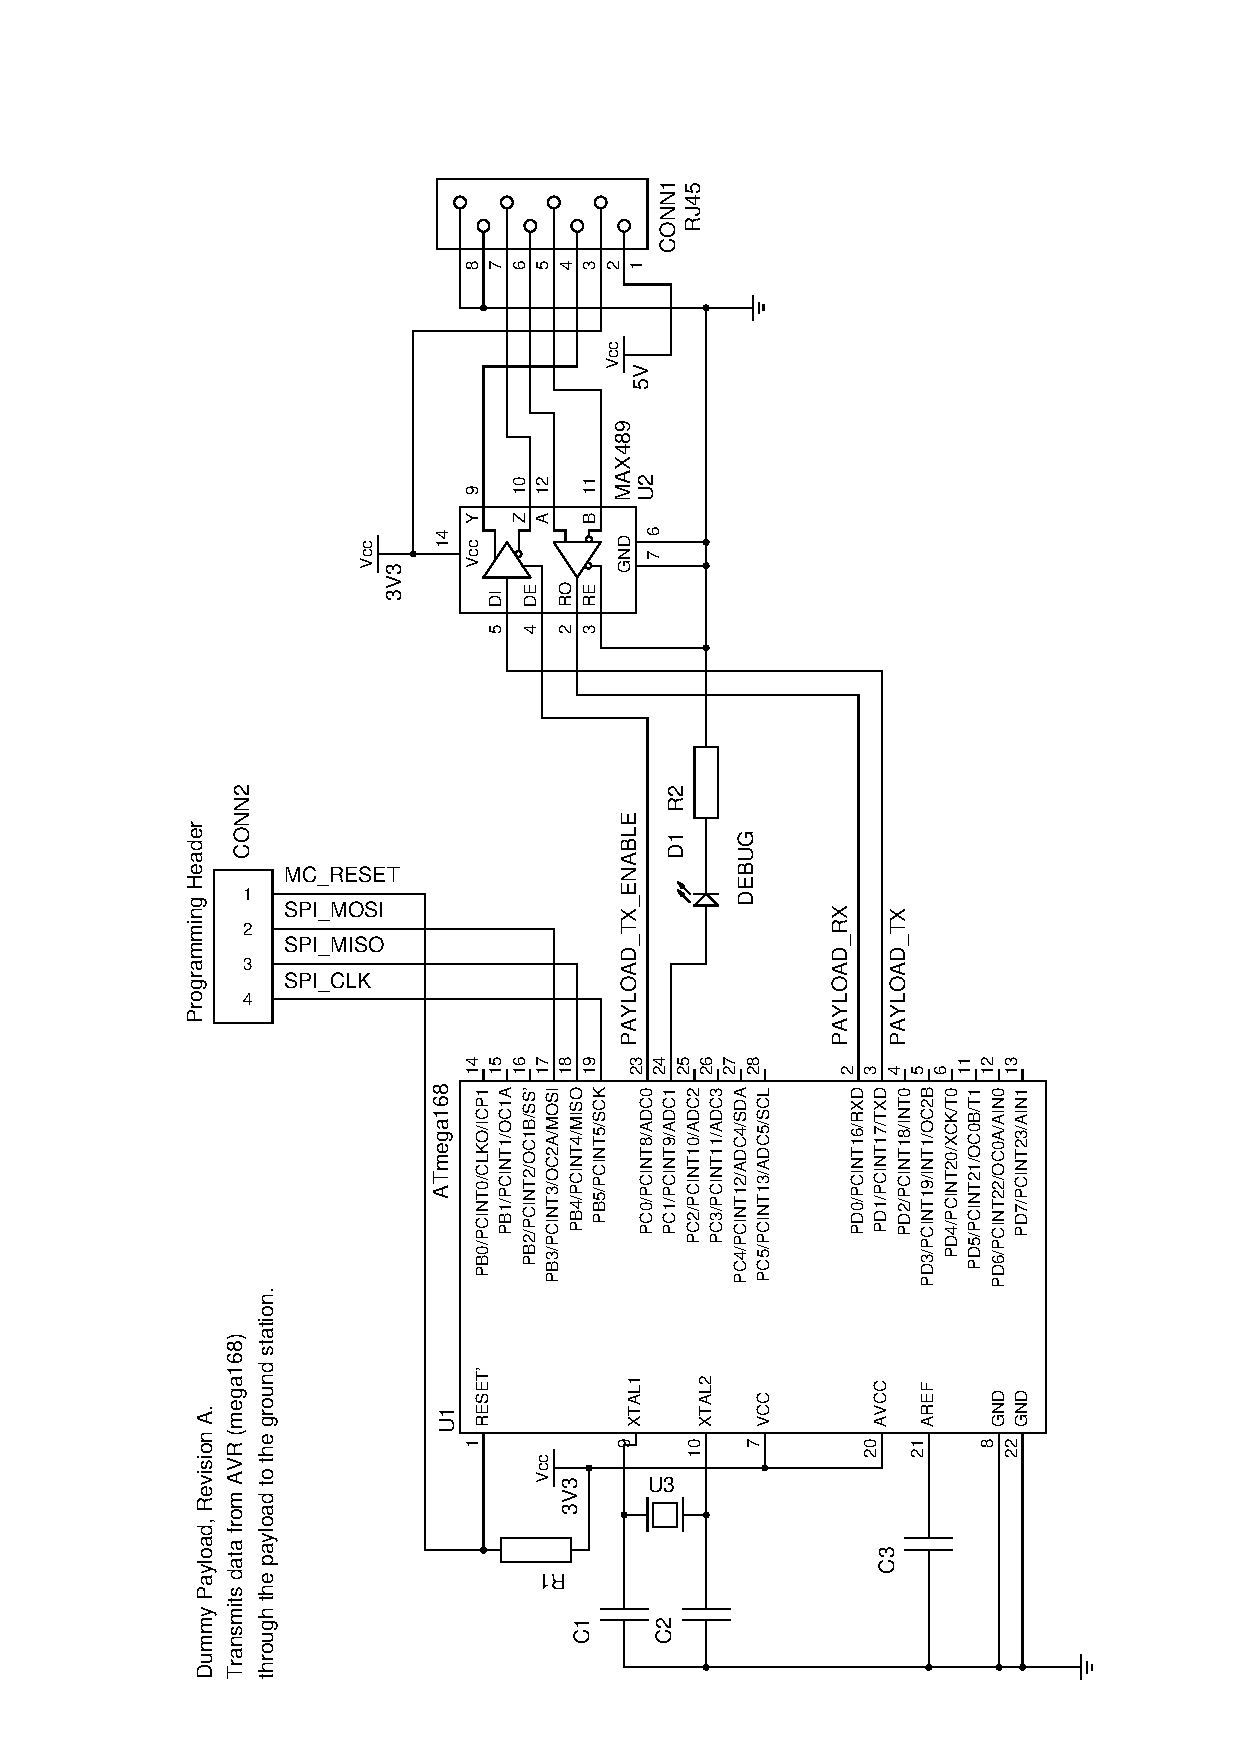
\includegraphics[width=1.4\textwidth, angle=90]{schematics/dummy_payload.pdf}
\caption{Schematic of the circuit used to test communication from a "dummy" 
payload to the autopilot module. Largely based on a schematic provided by 
our customer, and runs a slightly modified version of source code provided 
again, by our customer.}
\end{figure}

\section{Final Payload Module}
\label{Payload_Schematic}
\begin{figure}[H]
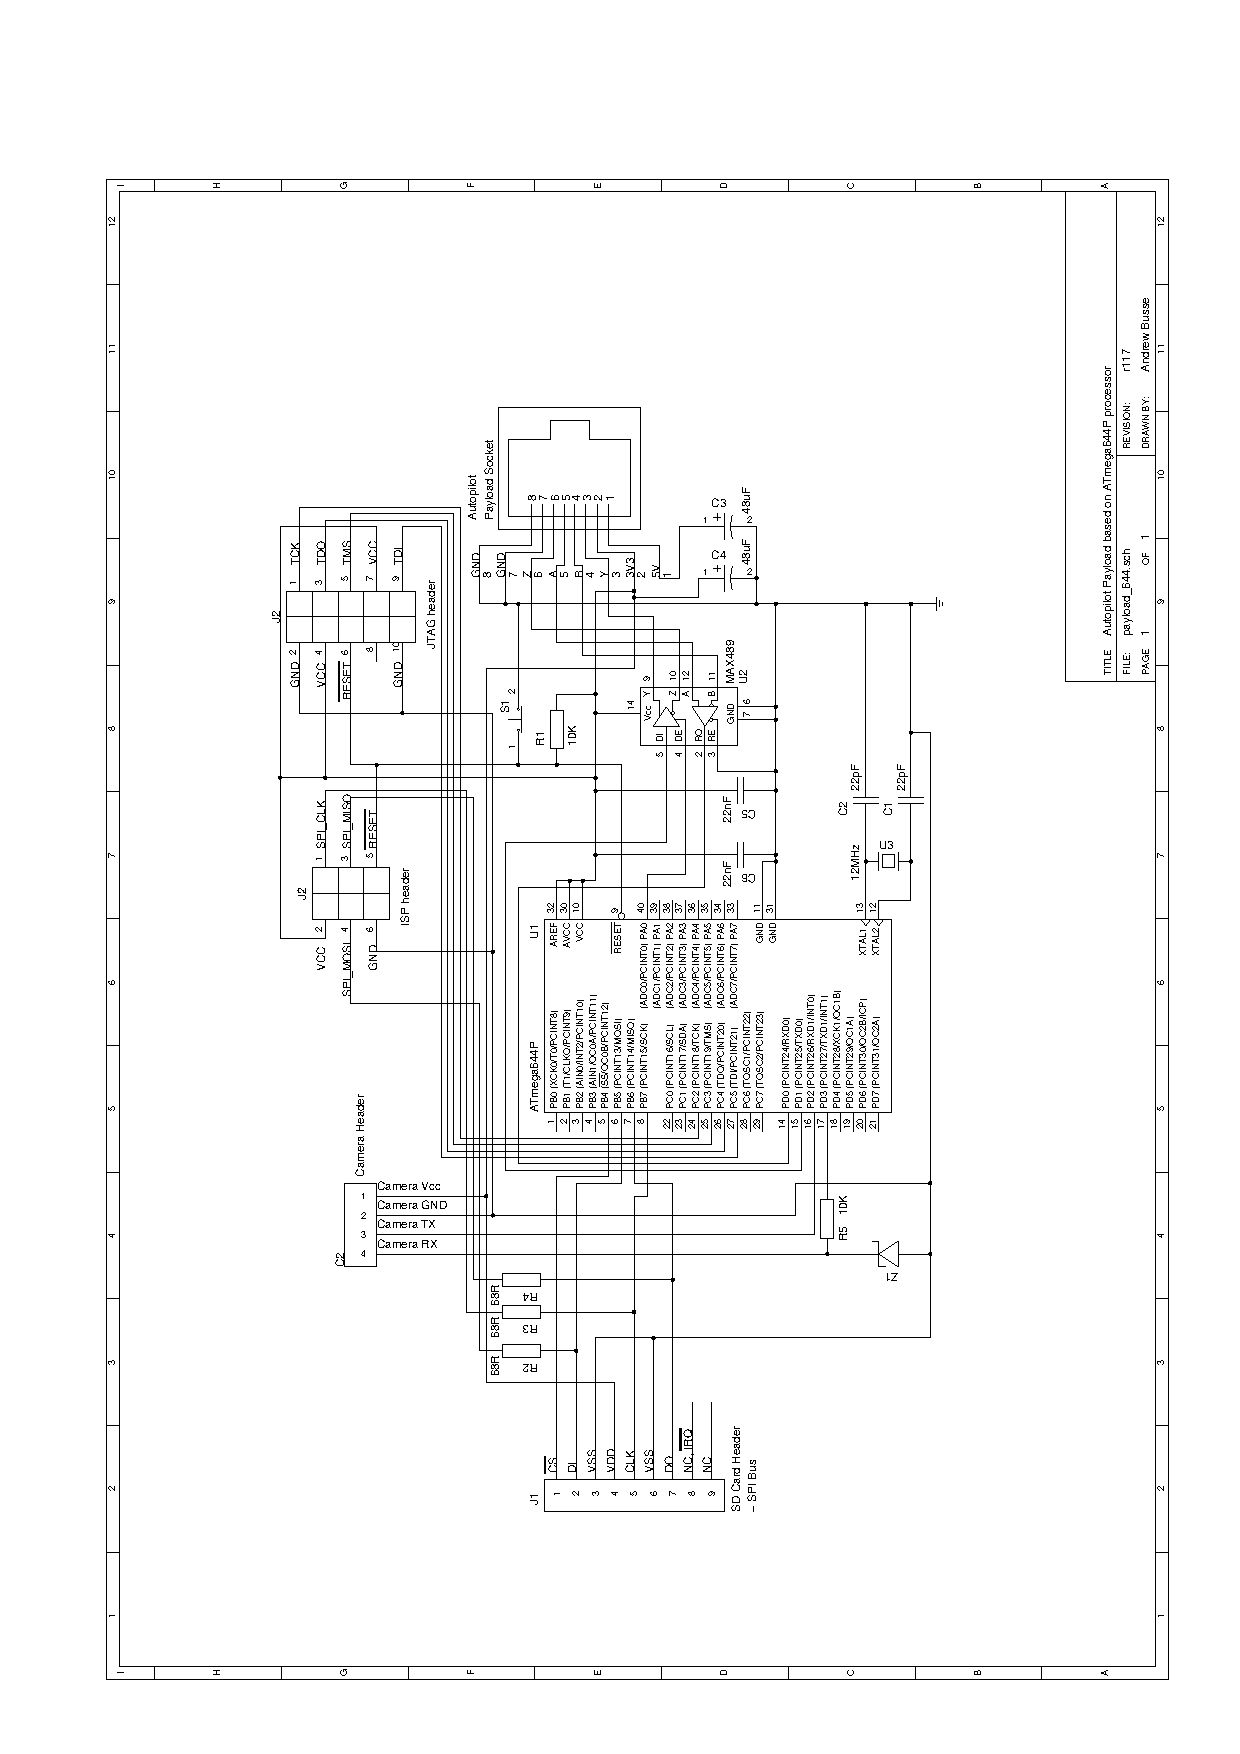
\includegraphics[width=1.4\textwidth, angle=90]{schematics/payload_644.pdf}
\caption{Final Schematic of the implemented payload module. See \ref{fig:PayloadImplementation} for a 
detailed explanation of which components are for what purpose}
\end{figure}

\section{Payload: Arduino Uno with additional ATmega168}
\begin{figure}[H]
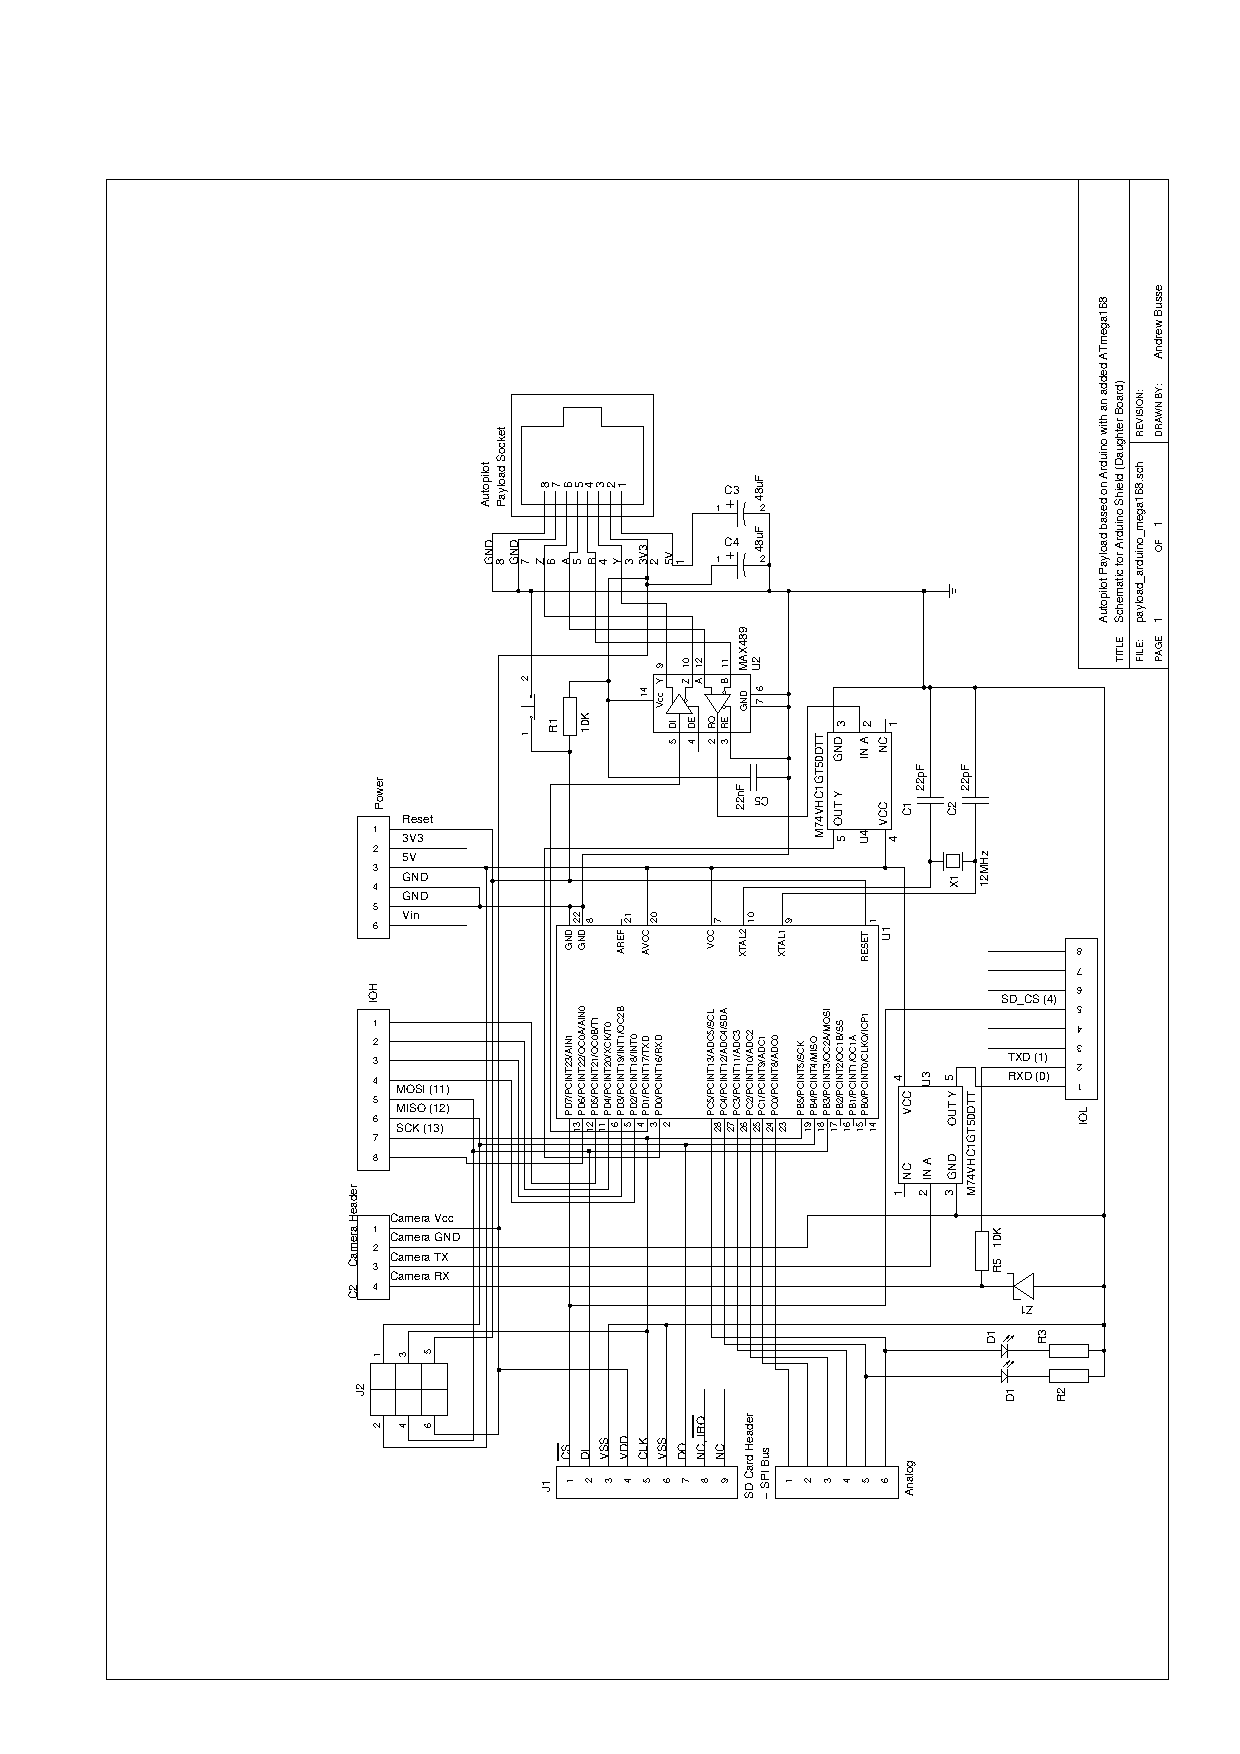
\includegraphics[width=1.4\textwidth, angle=90]{schematics/payload_arduino_mega168.pdf}
\caption{Schematic for a considered payload module: an 
Arduino Uno with a daughter board containing an ATmega168 for Autopilot to 
Payload module communication.}
\end{figure}

\section{Payload: Arduino Uno with Multiplexed UART line}
\begin{figure}[H]
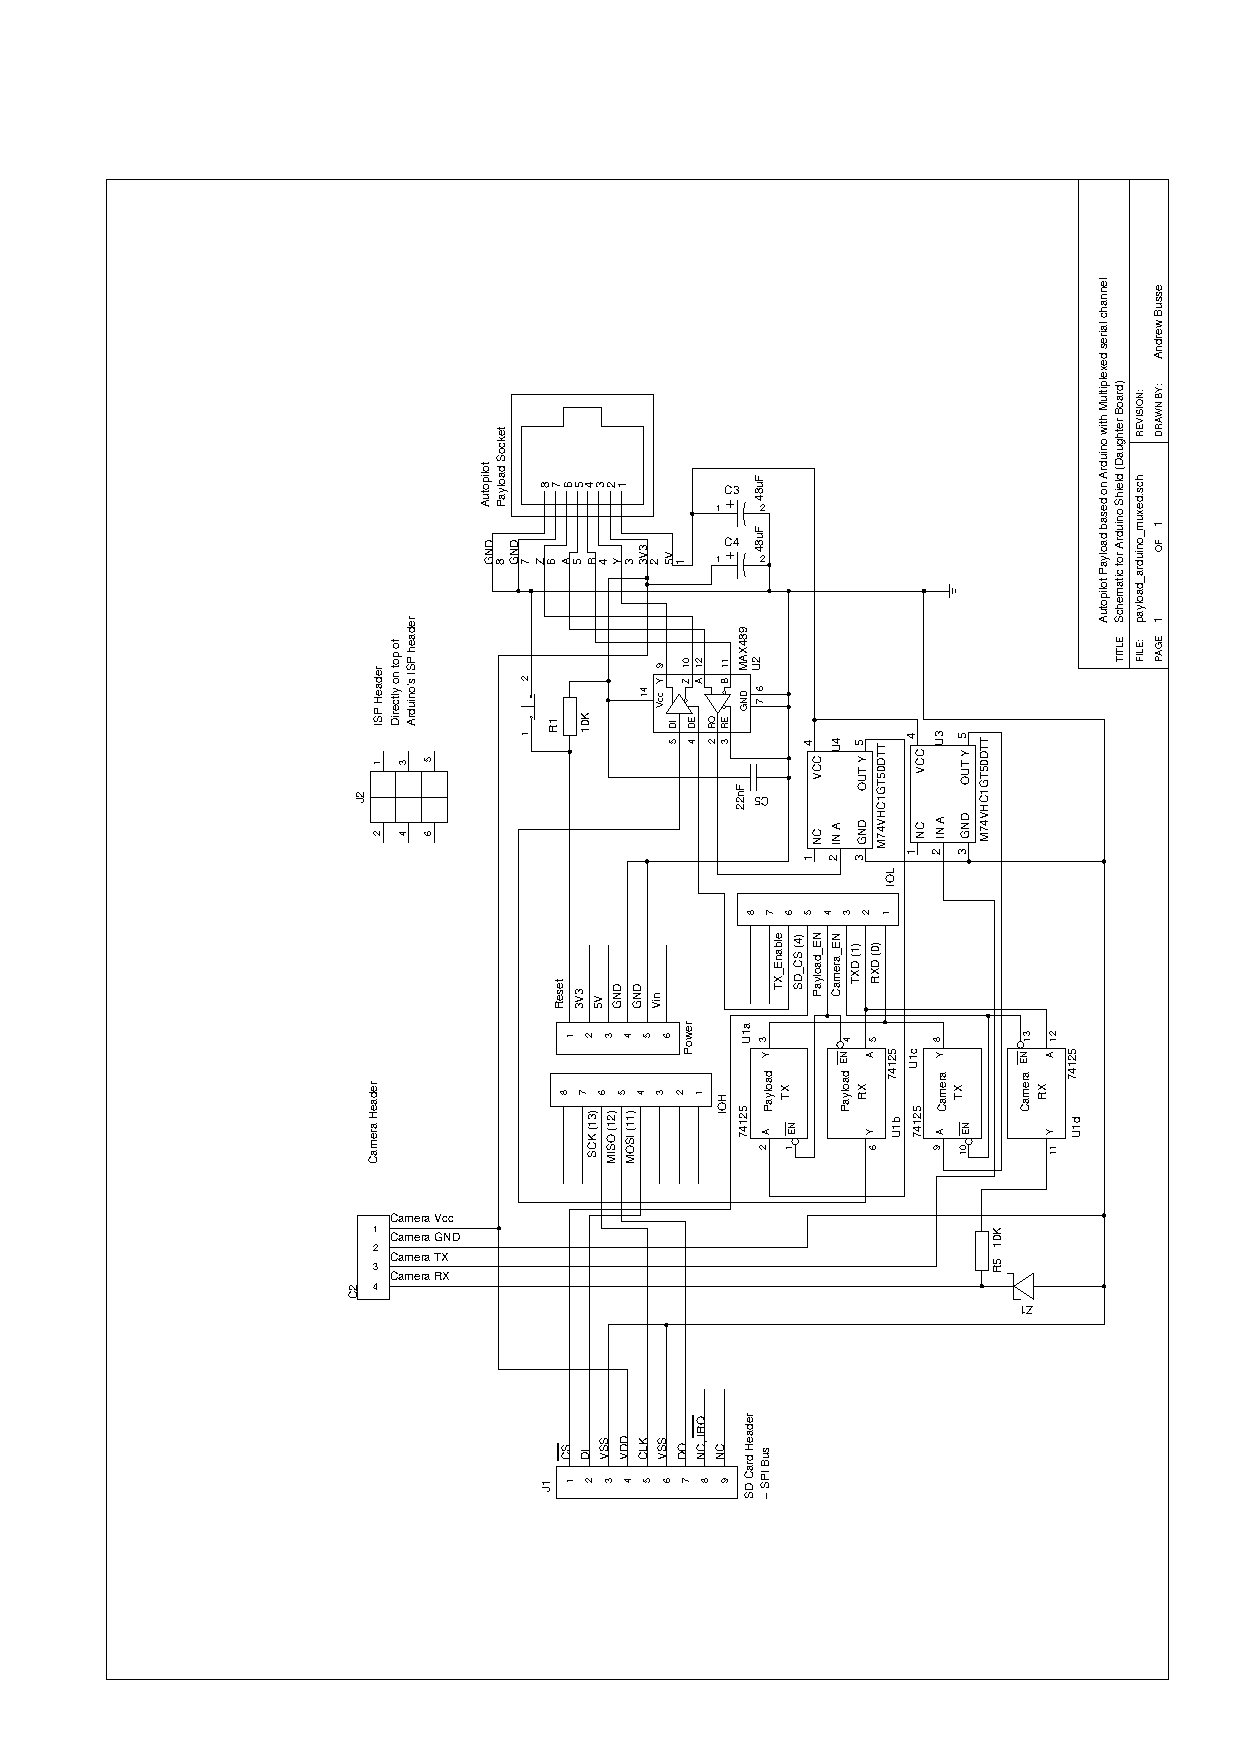
\includegraphics[width=1.4\textwidth, angle=90]{schematics/payload_arduino_muxed.pdf}
\caption{Schematic for a considered payload module: an 
Arduino Uno with its UART line multiplexed between camera and autopilot 
communication}
\end{figure}

\newpage

\chapter{PCB Layout}
% This is part of the FinalReport document.
% Copyright (C) 2011 Piyabhum Sornpaisarn, Andrew Busse, Michael Hodgson, John Charlesworth, Paramithi Svastisinha
% See the file COPYING in FinalReport/ for copying conditions.

\label{appendix-layout}

The layout of the final PCB module. As seen in figure \ref{fig:PayloadImplementation} 

This was made using PCB \footnote{\url{http://geda.seul.org/wiki/geda:gaf}} from the gEDA toolsuite.

Gerber files, and full source files, are available in our central GitHub 
\cite{github} repository, under schematics/payload\_644.pcb and schematics/gerbers

Running
\begin{verbatim} 
$ gsch2pcb projectrc
\end{verbatim}
from within schematics/ should update any changes you make to payload\_644.sch.

\begin{figure}[H]
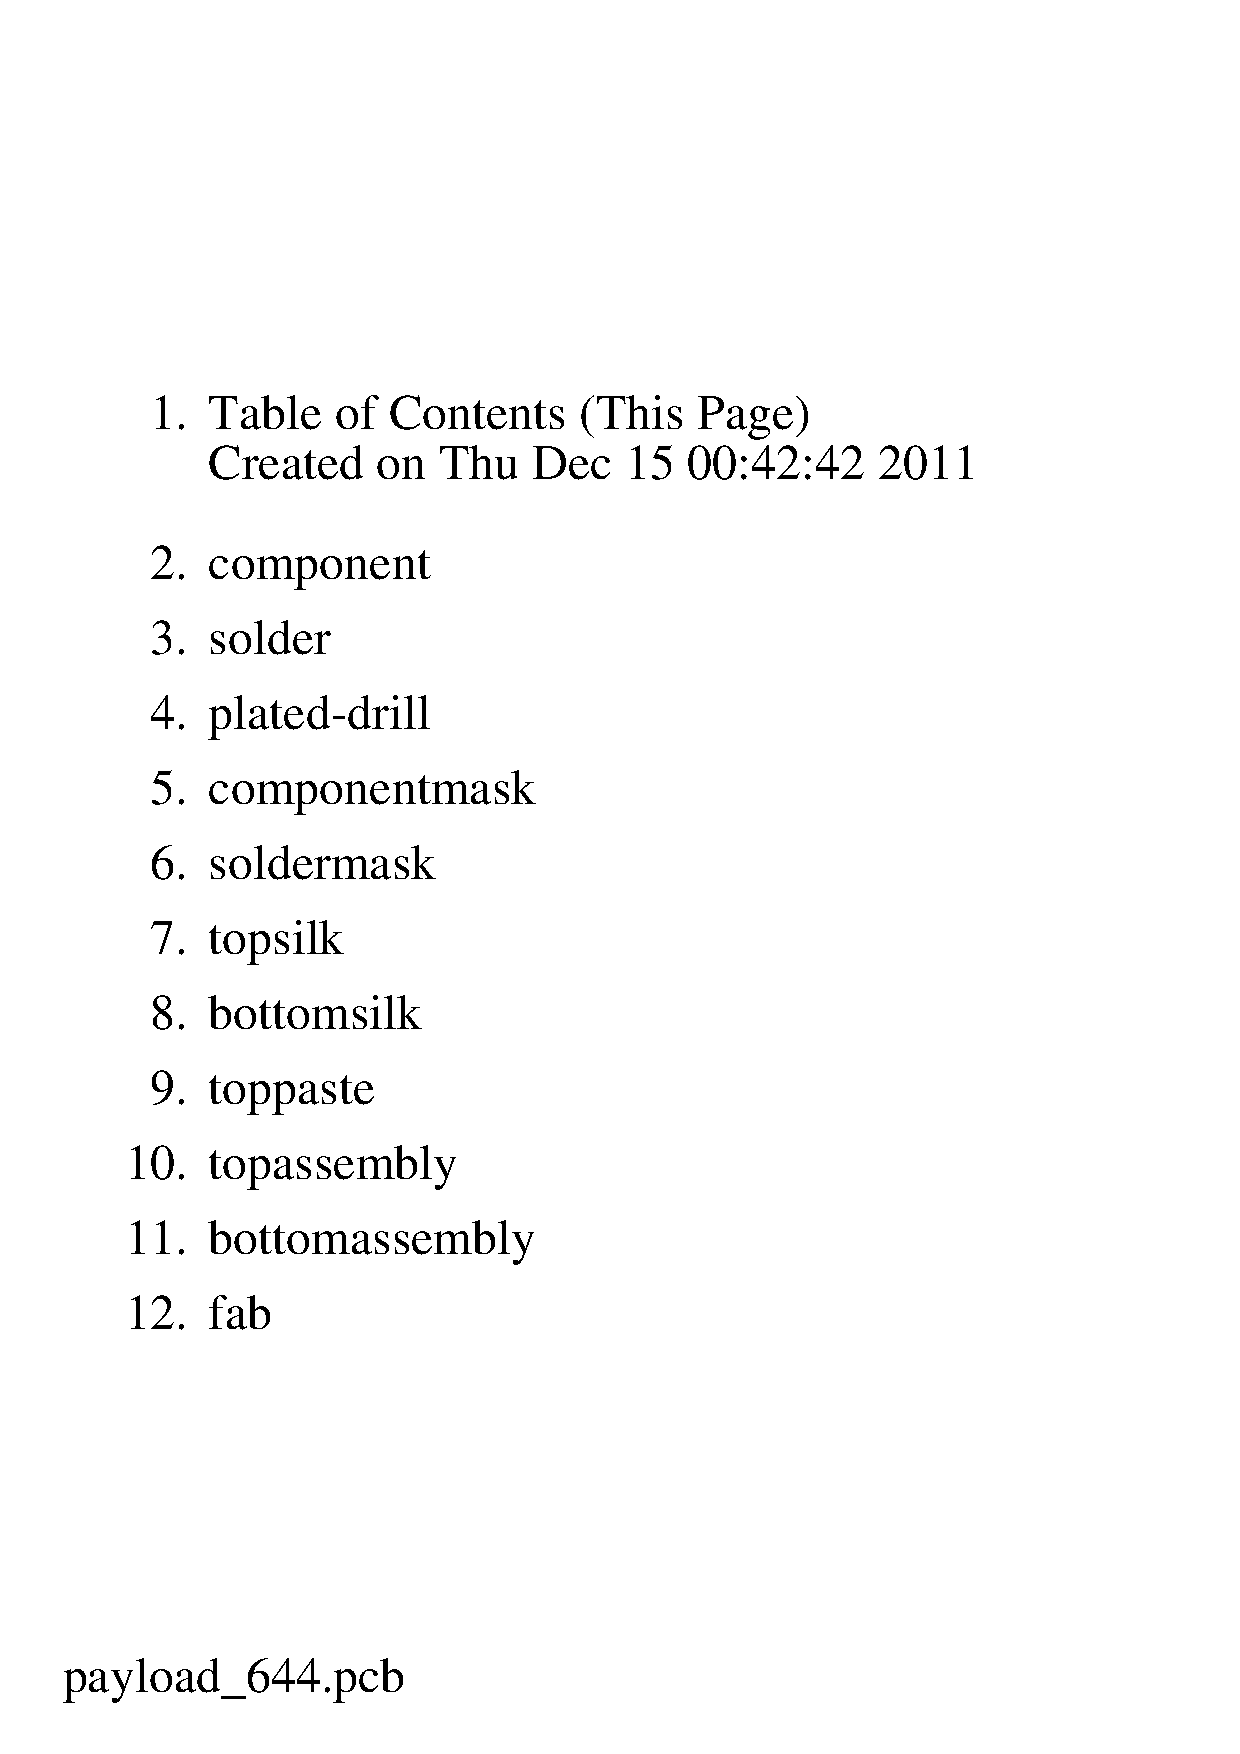
\includegraphics[width=1.4\textwidth, angle=90]{schematics/payload_644_layout.jpg}
\caption{Layout of our delivered PCB module. Dark Red: component layer. Light Blue: solder layer}
\end{figure}

\newpage

\chapter{Agreed Specification}
% This is part of the FinalReport document.
% Copyright (C) 2011 Piyabhum Sornpaisarn, Andrew Busse, Michael Hodgson, John Charlesworth, Paramithi Svastisinha
% See the file COPYING in FinalReport/ for copying conditions.

\label{initial_spec}

This Specification is our specification as it was submitted on to C-BASS 
on Monday 10th October 2011

\includepdf[scale=1.0,pages={1,2},offset=14mm -20mm]{spec/Agreed_Spec_GDP18.pdf}

\newpage

\chapter{Gantt Charts}
This section shows the Gantt Charts produced for this project. The first one, 
displayed over the first three pages, shows our initial Gantt chart, as 
produced for handin with the specification (10th October 2011).

The second, shown over pages 4 to 6, shows a revised version of our Gantt 
Chart, produced on 8th November 2011.

These Gantt Charts have been produced using the Planner tool from GNOME office.
\footnote{\url{http://live.gnome.org/Planner}}

%\includepdf[scale=1.0,pages={1-3},offset=25mm -25mm]{gantt/gantt1.pdf}
%\includepdf[scale=1.0,pages={1-3},offset=25mm -25mm]{gantt/gantt2.pdf}

\newpage

\chapter{User Documentation}
% This is part of the FinalReport document.
% Copyright (C) 2011 Piyabhum Sornpaisarn, Andrew Busse, Michael Hodgson, John Charlesworth, Paramithi Svastisinha
% See the file COPYING in FinalReport/ for copying conditions.

\label{userDocs}

\includepdf[scale=1.0,pages={1,2,3,4,5,6,7},offset=14mm -20mm]{docs/userGuide.pdf}

\newpage

\backmatter
\bibliographystyle{ecs}

% This is part of the FinalReport document.
% Copyright (C) 2011 Piyabhum Sornpaisarn, Andrew Busse, Michael Hodgson, John Charlesworth, Paramithi Svastisinha
% See the file COPYING in FinalReport/ for copying conditions.

\bibliographystyle{ecs}

\begin{thebibliography}{9}

	\bibitem{SkyCircuits} SkyCircuits Ltd. Web. 13th Dec. 2011 \url{http://www.skycircuits.com/}

	\bibitem{SULSA} SULSA \emph{The "Southampton University Laser Sintered Aircraft} Web. 13th Dec. 2011 \url{http://www.soton.ac.uk/~decode/index_files/Page804.htm}

	\bibitem{SC_Press} New Scientist \emph{3D printing: The world's first printed plane} Web. 13th Dec. 2011 \url{http://www.newscientist.com/article/dn20737-3d-printing-the-worlds-first-printed-plane.html}

	\bibitem{SC2} SkyCircuits \emph{SC2 autopilot module} Web. 14th Dec. 2011 \url{http://www.skycircuits.com/autopilot/sc2}

	\bibitem{tortorella_jpeg_enc} Tortorella, Richard. \emph{Image Doctoring: JPEG Encoding and Analysis}. Rep. NARCAP, May 2009. Web. 11 Oct. 2011. \url{http://www.narcap.org/reports/narcap_IR-01_DigHoaxing.pdf}.
	
	\bibitem{exif_std} Japan Electronics and Information Technology Industries Association (JEITA). \emph{Digital Still Camera Image File Format Standard (Exchangeable Image File Format for Digital Still Cameras: Exif)} Version 2.2. Tech. Japan Electronic Industry Development Association (JEIDA), 12 June 1998. Web. 14 Oct. 2011 \url{http://www.exif.org/Exif2-2.PDF}.
	
	\bibitem{netravali_digital_repr} Netravali, Arun N., and Barry G. Haskell. \emph{Digital Pictures: Representation and Compression}. New York: Plenum, 1988. Print. 
	
	\bibitem{jpeg_layout} \emph{JPEG File Layout and Format}. Original URL: \\http://www.funducode.com/freec/Fileformats/format3/format3b.htm (defunct).\\DCube Software Technologies, 5 July 2002. Web. 28 Oct. 2011. \url{http://class.ee.iastate.edu/ee528/Reading%20material/JPEG_File_Format.pdf}
	
	\bibitem{winzip_jpeg_compression} WinZip® International LLC. \emph{JPEG Compression}. Tech. Version 1.0. 11 Sept. 2008. Web. 28 Oct. 2011. \url{http://www.winzip.com/wz_jpg_comp.pdf}.
	
	\bibitem{poynton_chroma_subsampling} Poynton, Charles. \emph{Chroma Subsampling Notation.} Charles Poynton. 24 Jan. 2008. Web. 31 Oct. 2011. \url{http://poynton.com/PDFs/Chroma_subsampling_notation.pdf}.
	
	\bibitem{kerr_chroma_subsampling} Kerr, Douglas A. \emph{Chrominance Subsampling in Digital Images}. Rep. Issue 2. 3 Dec. 2009. Web. 31 Oct. 2011. \url{http://dougkerr.net/pumpkin/articles/Subsampling.pdf}.
	
	\bibitem{hass_impulse_jpeg} Hass, Calvin. \emph{ImpulseAdventure - Digital Photography Articles.} 2008. Web. 22 Nov. 2011. \url{http://www.impulseadventure.com/photo/}.
	
	\bibitem{ucam_datasheet} 4D Systems. \emph{uCam Serial JPEG Camera Module Data Sheet} 8 Jul. 2010. \url{http://www.4dsystems.com.au/downloads/micro-CAM/Docs/uCAM-DS-rev4.pdf}.

	\bibitem{software_serial} Arduino. \emph{SoftwareSerial Library.} Web. 9th Dec. 2011 \url{http://www.arduino.cc/en/Reference/SoftwareSerial}.

	\bibitem{arduino_sd_library} Arduino. \emph{SD Library.} Web. 10th Dec. 2011 \url{http://www.arduino.cc/en/Reference/SD}.
	
	\bibitem{arduino_serial_library} Arduino. \emph{Serial Library.} Web. 1st Dec. 2011 \url{http://www.arduino.cc/en/Reference/Serial}.

	\bibitem{atmega644p} Atmel. \emph{ATMega644P} Web. 10th Dec. 2011 \url{http://www.atmel.com/dyn/products/product_card.asp?part_id=3896}

	\bibitem{sanguino} Sanguino. \emph{What is Sanguino?} Web. 10th Dec. 2011 \url{http://sanguino.cc/}.

	\bibitem{mbed} mbed. \emph{Welcome to mbed!} Web. 10th Dec. 2011 \url{http://mbed.org/}.

	\bibitem{olimexino} Olimex. \emph{Olimexino-stm32 development board Users Manual} Web. Oct. 2011 \url{http://www.olimex.com/dev/DUINO/OLIMEXINO-STM32/OLIMEXINO-STM32.pdf}.

	\bibitem{github} Github. \emph{Our "Official", Central Repository} Web. 11th Dec. 2011 \url{https://github.com/uavcamera/uavcamera}

	\bibitem{go-naked} \emph{Spirit Circuits Go Naked} Web. 11th Dec. 2011 \url{http://www.spiritcircuits.com/services/go-naked}
	
	\bibitem{peak_netFrame} C.D. CĂLEANU, V. TIPONUŢ, I. BOGDANOV, S. IONEL, I. LIE \emph{C\# and .NET Framework for uC communication protocol Proceedings of the 11th WSEAS International Conference on COMPUTERS, Agios Nikolaos, Crete Island, Greece, July 26-28, 2007
implementation} 2008. Web. 22 Nov. 2011.
\url{www.wseas.us/e-library/conferences/2007cscc/papers/561-338.pdf}.

	\bibitem{tsuiK} Kakit Tsui \emph{Ad Hoc Network:Generic USB Device Driver Development} (2003)
\url{http://crisp.ece.cornell.edu/mengproj/alan_report.doc}.

	\bibitem{keithC} Keith Clark,Peter J. Robinson,Richard Hagen.(2001) Multi-threading and message communication in Qu-Prolog.\textit{Theory and Practice of Logic Programming} . 1 (3), p283-301 
	
	\bibitem{davidW} Keith Clark,Peter J. Robinson,Richard Hagen.(2004) \textit{Beginning .NET game programming in C\#.} United States of America: Apress. 

	\bibitem{xieX} Xiaoyun Xie.(2004) \textit{Distributed Objects System in C\#.} Rochester, United States of America. 

	\bibitem{davidB} David B. Makofske, Michael J. Donahoo, Kenneth L. Calvert.(2004) \textit{TCP/IP sockets in C\#  practical guide for programmers}. Amsterdam: Elsevier.

	\bibitem{normanM} Norman Matloff. (2009) \textit{Tutorial on Network Programming with Python}. California

	\bibitem{guidoR} Guido van Rossum. (1994) \textit{Extending and Embedding the Python Interpreter}. The Netherlands

	\bibitem{sannerM} M. F. SANNER. (1999) \textit{PYTHON: A PROGRAMMING LANGUAGE FOR SOFTWARE
INTEGRATION AND DEVELOPMENT}. California

	\bibitem{kennethC} Kenneth L. Calvert, Michael J. Donahoo. (2008) \textit{TCP/IP Sockets in Java
Practical Guide for Programmers}. Kentucky:Elsevier

	\bibitem{elliotH} Elliot R. Harold, Michael J. Donahoo. (1997) \textit{Java Network Programming}. USA:O'Reilly, p35

	\bibitem{ucam_test_software} 4D Systems. Web. 13th Dec. 2011. \url{http://www.4dsystems.com.au/prod.php?id=82}.

	\bibitem{robertH}Robert Harkness and Malcolm Crook and David Povey.(2007) \textit{Programming Review of Visual Basic.NET for the Laboratory Automation Industry}. Journal of the Association for Laboratory Automation vol.12, p.25-32.
	\url{http://www.sciencedirect.com/science/article/pii/S1535553506005302}.

	\bibitem{gpl} GNU \emph{The GNU Public License version 3} Web. 14th Dec. 2011 \url{http://www.gnu.org/licenses/gpl-3.0.html}

	\bibitem{ccbysa} Creative Commons \emph{Attribution-ShareAlike 2.0 UK: England \& Wales (CC BY-SA 2.0)} Web. 14th Dec. 2011. \url{http://creativecommons.org/licenses/by-sa/2.0/uk/}
	
	\bibitem{fdl} GNU \emph{The GNU Free Documentation License version 1.3} Web. 14th Dec. 2011. \url{http://www.gnu.org/copyleft/fdl.html}

	\bibitem{Huffman} D.A. Huffman \textit{A Method for the Construction of Minimum-Redundancy Codes}. Proceedings of the I.R.E. Sept. 1952. p1098-p1102


	\bibitem{avr_param} Atmel.\textit{megaAVR Parameters} 15th Dec. 2011. \url{http://www.atmel.com/dyn/products/param_table.asp?category_id=163&family_id=607&subfamily_id=760}

	\bibitem{flash_datasheet} \emph{A25L040-U - 16Mbit Low Voltage, Serial Flash Memory With 100MHz Uniform 4KB Sectors - AMIC Technology} 8 Jul. 2010. \url{http://pdf1.alldatasheet.com/datasheet-pdf/view/244476/AMICC/A25L040-U.html}.


\end{thebibliography} 

\newpage
\chapter{Glossary}

\section*{Terms} 
\begin{description}
	\item[YCbCr] Colour space used to represent JPEG images. Composed of three values:
		\begin{description}
			\item[Y] luma component.
			\item[Cb] blue-difference chroma component.
			\item[Cr] red-difference chroma component.
		\end{description}
	\item[4:x:y]Chroma subsampling notation.
		\begin{description}
			\item[4] Luma horizontal (and vertical) sampling reference.
			\item[x] Cb and Cr horizontal sampling factor.
			\item[y] Cb and Cr horizontal sampling factor. If 0, indicates 2:1 vertical subsampling for both Cb and Cr.
		\end{description}
\end{description}

\section*{Abbreviations} 
\begin{description}
	\item[AC] Alternating Current 
	\item[DC] Digital Current 
	\item[JPEG] Joint Photographic Experts Group, creators of the jpeg compression method. Used interchangeably with the jpeg image type.
	\item[EXIF] EXchangeable Image File format for digital still cameras.
	\item[MCU] Minimum Coded Unit
	\item[DFT] Discrete Fourier Transform
	\item[FFT] Fast Fourier Transform
	\item[DCT] Discrete Cosine Transform
	\item[WHT] Walsh–Hadamard Transform
	\item[KLT] Karhunen-Lo\`eve Transform
	\item[SOI] Start Of Image
	\item[SOF] Start Of Frame
	\item[DHT] Define Huffman Table(s)
	\item[HT] Huffman Table
	\item[DQT] Define Quantization Table(s)
	\item[QT] Quantization Table
	\item[SOS] Start Of Scan
	\item[EOI] End Of Image
	\item[SD card]
\end{description}

\newpage

Copyright \copyright 2011 Piyabhum Sornpaisarn, Andrew Busse, Michael Hodgson, John Charlesworth, Paramithi Svastisinha

Permission is granted to copy, distribute and/or modify this
document under the terms of the GNU Free Documentation License,
Version 1.3 or any later version published by the Free Software
Foundation; with no Invariant Sections, no Front-Cover Texts and
no Back-Cover Texts.  A copy of the license is included in the
file entitled "COPYING".

\end{document}
%% ----------------------------------------------------------------
